\documentclass[12pt]{article}
\usepackage[utf8]{inputenc}
\usepackage[spanish]{babel}
\usepackage{siunitx}
% ---------------------------------------------------
% 						FONT 
% ---------------------------------------------------

\usepackage{cmbright}								% Font
\documentclass{article}
\usepackage{siunitx}
\usepackage{hyperref} % LINKS
\usepackage{caption}
\decimalpoint
\usepackage{mathtools}
\usepackage{amsmath}
\usepackage{amsthm}
\usepackage{amssymb}
\usepackage{graphicx}
\usepackage[margin=0.9in]{geometry}
\usepackage{fancyhdr}
\usepackage[inline]{enumitem}
\usepackage{float}
\usepackage{cancel}
\usepackage{bigints}
\usepackage{color}
\usepackage{xcolor}
\usepackage{listingsutf8}
\usepackage{algorithm}
\usepackage{tocloft}
\usepackage[none]{hyphenat}
\usepackage{graphicx}
\usepackage{grffile}
\usepackage{tabularx}
\usepackage[nottoc,notlot,notlof]{tocbibind}
\usepackage{times}
\usepackage{color}
\usepackage{enumitem}
\usepackage{amsfonts}
\definecolor{gray97}{gray}{.97}
\definecolor{gray75}{gray}{.75}
\definecolor{gray45}{gray}{.45}
\renewcommand{\cftsecleader}{\cftdotfill{\cftdotsep}}
\pagestyle{fancy}
\setlength{\headheight}{15pt} 
\lhead{Práctica 3: Amplificador de Instrumentación}
\rhead{\thepage}
\lfoot{ESCOM-IPN}
\renewcommand{\footrulewidth}{0.5pt}
\setlength{\parskip}{0.5em}
\newcommand{\ve}[1]{\overrightarrow{#1}}
\newcommand{\abs}[1]{\left\lvert #1 \right\lvert}
\date{ 01 de Junio 2018}
\title{Amplificador}
\author{Instrumentacion}
\usepackage[
  separate-uncertainty = true,
  multi-part-units = repeat
]{siunitx}

\definecolor{pblue}{rgb}{0.13,0.13,1}
\definecolor{pgreen}{rgb}{0,0.5,0}
\definecolor{pred}{rgb}{0.9,0,0}
\definecolor{pgrey}{rgb}{0.46,0.45,0.48}
\lstset{tabsize=1}
\usepackage{wrapfig}
\usepackage{multicol}
\usepackage{listings}
\lstset{ frame=Ltb,
framerule=0pt,
aboveskip=0.5cm,
framextopmargin=3pt,
framexbottommargin=3pt,
framexleftmargin=0.4cm,
framesep=0pt,
rulesep=.4pt,
backgroundcolor=\color{gray97},
rulesepcolor=\color{black},
%
stringstyle=\ttfamily,
showstringspaces = false,
basicstyle=\small\ttfamily,
commentstyle=\color{gray45},
keywordstyle=\bfseries,
%
numbers=left,
numbersep=15pt,
numberstyle=\tiny,
numberfirstline = false,
breaklines=true,
}

% minimizar fragmentado de listados
\lstnewenvironment{listing}[1][]
{\lstset{#1}\pagebreak[0]}{\pagebreak[0]}

\lstdefinestyle{consola}
{basicstyle=\scriptsize\bf\ttfamily,
backgroundcolor=\color{gray75},
}

\lstdefinestyle{Java}
{language=Java,
}

%%%%%%%%%%%%%%%%%%%%%

\lstdefinestyle{customc}{
  belowcaptionskip=1\baselineskip,
  breaklines=true,
  frame=L,
  xleftmargin=\parindent,
  language=C,
  showstringspaces=false,
  basicstyle=\footnotesize\ttfamily,
  keywordstyle=\bfseries\color{green!40!black},
  commentstyle=\itshape\color{purple!40!black},
  identifierstyle=\color{blue},
  stringstyle=\color{orange},
}

\lstdefinestyle{customasm}{
  belowcaptionskip=1\baselineskip,
  frame=L,
  xleftmargin=\parindent,
  language=[x86masm]Assembler,
  basicstyle=\footnotesize\ttfamily,
  commentstyle=\itshape\color{purple!40!black},
}

\lstset{escapechar=@,style=customc}

% Ayuda para el formato de las tablas
\usepackage{array}
% Se declara un nuevo tipo de columna para alinear de manera:
% -Horizontal
\newcolumntype{P}[1]{>{\centering\arraybackslash}p{#1}}
% -Vertical
\newcolumntype{M}[1]{>{\centering\arraybackslash}m{#1}}

% Indica la separacion entre las columnas de una tabla
\setlength{\tabcolsep}{10pt} % Default value: 6pt
% Indica el padding inferior y superior de las celdas de una tabla
\renewcommand{\arraystretch}{1.8} % Default value: 1

\usepackage{longtable}
%Permite crear columnas en el documento
\usepackage{multicol} 
\usepackage{color}
\usepackage{comment}
\newcommand{\tabitem}{~~\llap{\textbullet}~~}
\newcommand{\subtabitem}{~~~~\llap{\textbullet}~~}

\bibliographystyle{IEEEtran}
\begin{document}
		\begin{titlepage}
			\begin{center}
				
				% Upper part of the page. The '~' is needed because \\
				% only works if a paragraph has started.
				
				\noindent
				\begin{minipage}{0.5\textwidth}
					\begin{flushleft} \large
						\includegraphics[width=0.5\textwidth]{../ipn.png}
					\end{flushleft}
				\end{minipage}%
				\begin{minipage}{0.55\textwidth}
					\begin{flushright} \large
						\includegraphics[width=0.4\textwidth]{../escom.png}
					\end{flushright}
				\end{minipage}
				
				\textsc{\LARGE Instituto Politécnico Nacional}\\[0.5cm]
				
				\textsc{\Large Escuela Superior de Cómputo}\\[1cm]
				
				% Title
				
				{ \huge Práctica 3: Amplificador de Instrumentación \\[1cm] }
				
				{ \Large Unidad de aprendizaje: Instrumentación} \\[1cm]
				
				{ \Large Grupo: 3CM4 } \\[1cm]
				
				\noindent
				\begin{minipage}{0.5\textwidth}
					\begin{flushleft} \large
						\emph{Integrantes:}\\
						
						\begin{tabular}{ll}
						Aguilar Herrera Arianna Itzamina \\
					    Nicolás Sayago Abigail\\
					    Ramos Diaz Enrique \\
					\end{tabular}
					\end{flushleft}
				\end{minipage}%
				\begin{minipage}{0.5\textwidth}
					\begin{flushright} \large
						\emph{Profesor(a):} \\
						Tellez Barrera Juan Carlos  \\
					\end{flushright}
				\end{minipage}
				
				\vfill
				
				% Bottom of the page
				{\large Fecha de entrega: 05 de octubre de 2018}
			\end{center}
		\end{titlepage}
	
	\tableofcontents
	\newpage
	
	% /////////////////////////////////////////////////////////////////////
	%							OBJETIVOS
	% ////////////////////////////////////////////////////////////////////
	\section{Objetivo}
	\begin{itemize}
	    \item[\checkmark] Comprobar el uso del amplificador de instrumentación en la medición de una variable fisiológica, en este caso una señal mioeléctrica.
	\end{itemize}
	
	% /////////////////////////////////////////////////////////////////////
	%							MATERIAL
	% ////////////////////////////////////////////////////////////////////
	\begin{multicols}{2}
	\section{Material}
	\begin{itemize}
	    \item 1 Tablilla experimental (ProtoBoard)
	    \item 5 Amplificadores operacionales
	    \item 4 Resistores de $47 k\Omega$
	    \item 2 Resistores de $27 k\Omega$
	    \item 2 Resistores de $2.7 k\Omega$
	    \item 1 Resistor de $1 k\Omega$
	    \item 1 Resistor de $270 k\Omega$
	    \item 1 Resistor de $1 M\Omega$
	    \item 1 Capacitor de $100 nF$
	\end{itemize}
	
		% /////////////////////////////////////////////////////////////////////
	%							EQUIPO
	% ////////////////////////////////////////////////////////////////////
	\columnbreak
	\section{Equipo}
	\begin{itemize}
	    \item 1 Fuente de alimentación triple)
	    \item 1 Multímetro Digital o Analógico
	    \item Osciloscopio de propósito general
	    \item 4 Cables caimán - caimán
	    \item 4 Cables banana - banana
	    \item 2 Cables BNC - caimán
	    \end{itemize}
	    \end{multicols}
	
	% /////////////////////////////////////////////////////////////////////
	%							INTRODUCCION
	% ////////////////////////////////////////////////////////////////////

	\section{Introducción}
	\subsection{Señales mioeléctricas y Electromiogramas}
	Las señales electromiográficas (EMG) son señales eléctricas producidas por un músculo durante el proceso de contracción y relajación.
	
	        \begin{figure}[h!]
                \centering
                \includegraphics[scale=0.5]{Practica3/images/brazo1.jpg}
            \end{figure} 
	
	La señal mioeléctrica o señal EMG estará corrupta con ruido proveniente por varias fuentes, entre estas predomina la frecuencia de 60Hz de la línea eléctrica y ruido blanco existente en el ambiente. 
	
	La fuerza de contracción muscular total se incrementa por medio de dos mecanismos: el reclutamiento de unidades motoras previamente inactivas y el incremento de la frecuencia de descarga de unidades ya activas. 
	
	La señal mioeléctrica es la integración temporal y espacial de todos los potenciales de acción de la unidad motora detectados utilizando uno o dos electrodos a partir de un cierto volumen de tejido. La señal mioeléctrica, cuando se amplifica y se registra, se denomina electromiograma, y el proceso de obtención, procesamiento y análisis de señales electromiografías (EMG) se denomina electromiografía. 
	
		\begin{figure}[h!]
                \centering
                \includegraphics[scale=1.1]{Practica3/images/electromiograma.png}
    \end{figure} 
	
	Las señales EMG tienen una frecuencia que oscila entre \textbf{50 y 150 Hz.}

	Un electromiograma (EMG) mide la actividad eléctrica de los músculos cuando están en reposo y cuando se están usando. Es la técnica de registro gráfico de la actividad eléctrica producida por los músculos esqueléticos. 
	
	Los nervios controlan los músculos del cuerpo con señales eléctricas llamadas impulsos. 
	
	Durante el estudio, una o más agujas pequeñas (electrodos intramusculares) se introducen en el músculo a través de la piel, o se colocan electrodos en la superficie de la piel sobre el músculo (electrodos superficiales). 
	
	La actividad eléctrica que captan los electrodos se muestra en un osciloscopio (un monitor que muestra la actividad eléctrica en forma de ondas). Un amplificador de sonido se usa para poder oír la actividad.
	
	La electromiografía mide la actividad eléctrica del músculo en reposo, en una contracción leve y en una contracción enérgica. El tejido muscular normalmente no produce señales eléctricas durante el reposo. Cuando se introduce un electrodo, se puede observar un breve período de actividad en el osciloscopio pero, luego, no debería haber ninguna señal.
	
	Después de que se han colocado todos los electrodos, se debe contraer el músculo. El potencial de acción (el tamaño y la forma de la onda) que esta contracción crea en el osciloscopio proporciona información sobre la capacidad del músculo de responder cuando los nervios reciben estimulación. Cuando usted contrae el músculo más enérgicamente, se activan más y más fibras, produciendo potenciales de acción.
	
	\begin{figure}[h!]
                \centering
                \includegraphics[scale=0.3]{Practica3/images/emg.jpg}
    \end{figure} 
    
    \subsubsection{Voltajes típicos}
    La amplitud de las señales de EMG depende de varios factores; la posición, el tipo y material de los electrodos usados.
    
    Una típica señal de EMG tiene rangos de amplitud que van desde 0.1 a 0.5 mV. 
    
    \subsubsection{¿Para que sirve?}
    La electromiografía suele usarse junto con el estudio de conducción nerviosa para detectar la diferencia entre un trastorno muscular y un trastorno nervioso. La electromiografía detecta enfermedades que surgen de problemas con el músculo en sí. La electromiografía también detecta otros problemas que son consecuencia de cómo influyen en los músculos otros sistemas, como los nervios.
    
    La electromiografía puede realizarse para identificar la causa de los síntomas, por ejemplo, debilidad muscular, deformidad, elasticidad, atrofia y rigidez. También puede emplearse para detectar si una persona tiene verdadera debilidad muscular o si la debilidad es a causa del dolor o por motivos psicológicos.
    
    La electromiografía puede usarse para evaluar muchos problemas o trastornos, entre los cuales se incluyen los siguientes:
    \begin{itemize}
        \item Enfermedades neuromusculares
        \item Problemas de motricidad
        \item Compresión o lesión de los nervios
        \item Degeneración de músculos
    \end{itemize}
    
    \subsection{Amplificador de Instrumentación}
    El amplificador de instrumentación tiene todas las características del amplificador operacional:
    \begin{enumerate}
        \item Son amplificadores diferenciales con una ganancia diferencial precisa y estable, generalmente en el rango de 1 a 1000.
        \item Su ganancia diferencial se controlada mediante un único elemento analógicos (potenciómetro resistivo) o digital (conmutadores) lo que facilita su ajuste.
        \item Su ganancia en modo común debe ser muy baja respecto de la ganancia diferencial, esto es, debe ofrecer un CMRR muy alto en todo el rango de frecuencia en que opera.
        \item Una impedancia muy alta para que su ganancia no se vea afectada por la impedancia de la fuente de entrada.
        \item Una impedancia de salida muy baja para que su ganancia no se vea afectada por la carga que se conecta a su salida.
        \item Bajo nivel de las tensión de offset del amplificador y baja deriva en el tiempo y con la temperatura, a fin de poder trabajar con señales de continua muy pequeñas.
        \item Una anchura de banda ajustada a la que se necesita en el diseño.
        \item Un factor de ruido muy próximo a la unidad, Esto es, que no incremente el ruido.
        \item Una razón de rechazo al rizado a la fuente de alimentación muy alto.
    \end{enumerate}

    	\begin{figure}[h!]
                \centering
                \includegraphics[scale=1]{Practica3/images/amplificador.jpg}
    \end{figure} 
    
    Un amplificador de instrumentación tiene dos entradas, V+ y V-, una salida $V_{O}$ y una tierra común. Idealmente la ganancia diferencial $G\pm$ está dada por:
    
    $$G_{\pm} = \frac{V_{o}}{V_{+} - V_{-}}$$
    
    Para el circuito de la figura  la expresión de esta ganancia diferencial es:
    
    $$G_{\pm} = \frac{R_{4}}{R_{3}}\left[1 + \frac{2R_{2}}{R_{1}}\right]$$
    
    Una característica importante en el amplificador de instrumentación es la \textit{Relación de Rechazo de Modo Común},  la misma se define como la capacidad del amplificador de rechazar las señales de interferencia comunes (ruido) a ambas entradas y amplificar únicamente la diferencia entre las entradas. Un amplificador de instrumentación tiene tanto \textit{ganancia diferencial}, como la mostrada arriba ($G\pm$) y \textit{ganancia de modo común} $G_{C}$.
    
    $$ RRMC = 20log_{10}\left(\frac{G_{\pm}}{G_{C}}\right)$$


	% /////////////////////////////////////////////////////////////////////
	%							DESARROLLO
	% ////////////////////////////////////////////////////////////////////
    \newpage
	\section{Desarrollo}
	\subsection{PE 1 - Circuito 1}
	\subsubsection{Esquema}
	\begin{figure}[h!]
                \centering
                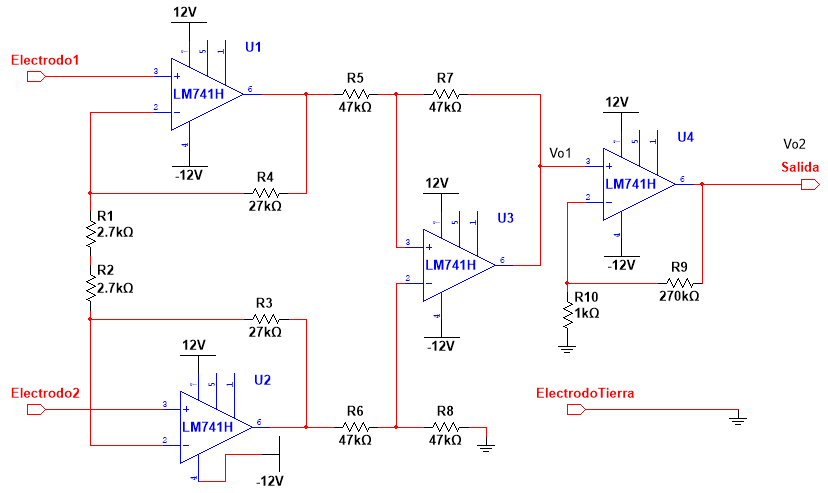
\includegraphics[width=\textwidth]{Practica3/images/ccircuito1.PNG}
    \end{figure} 
    
	\subsubsection{Circuito cableado}
		\begin{figure}[h!]
                \centering
                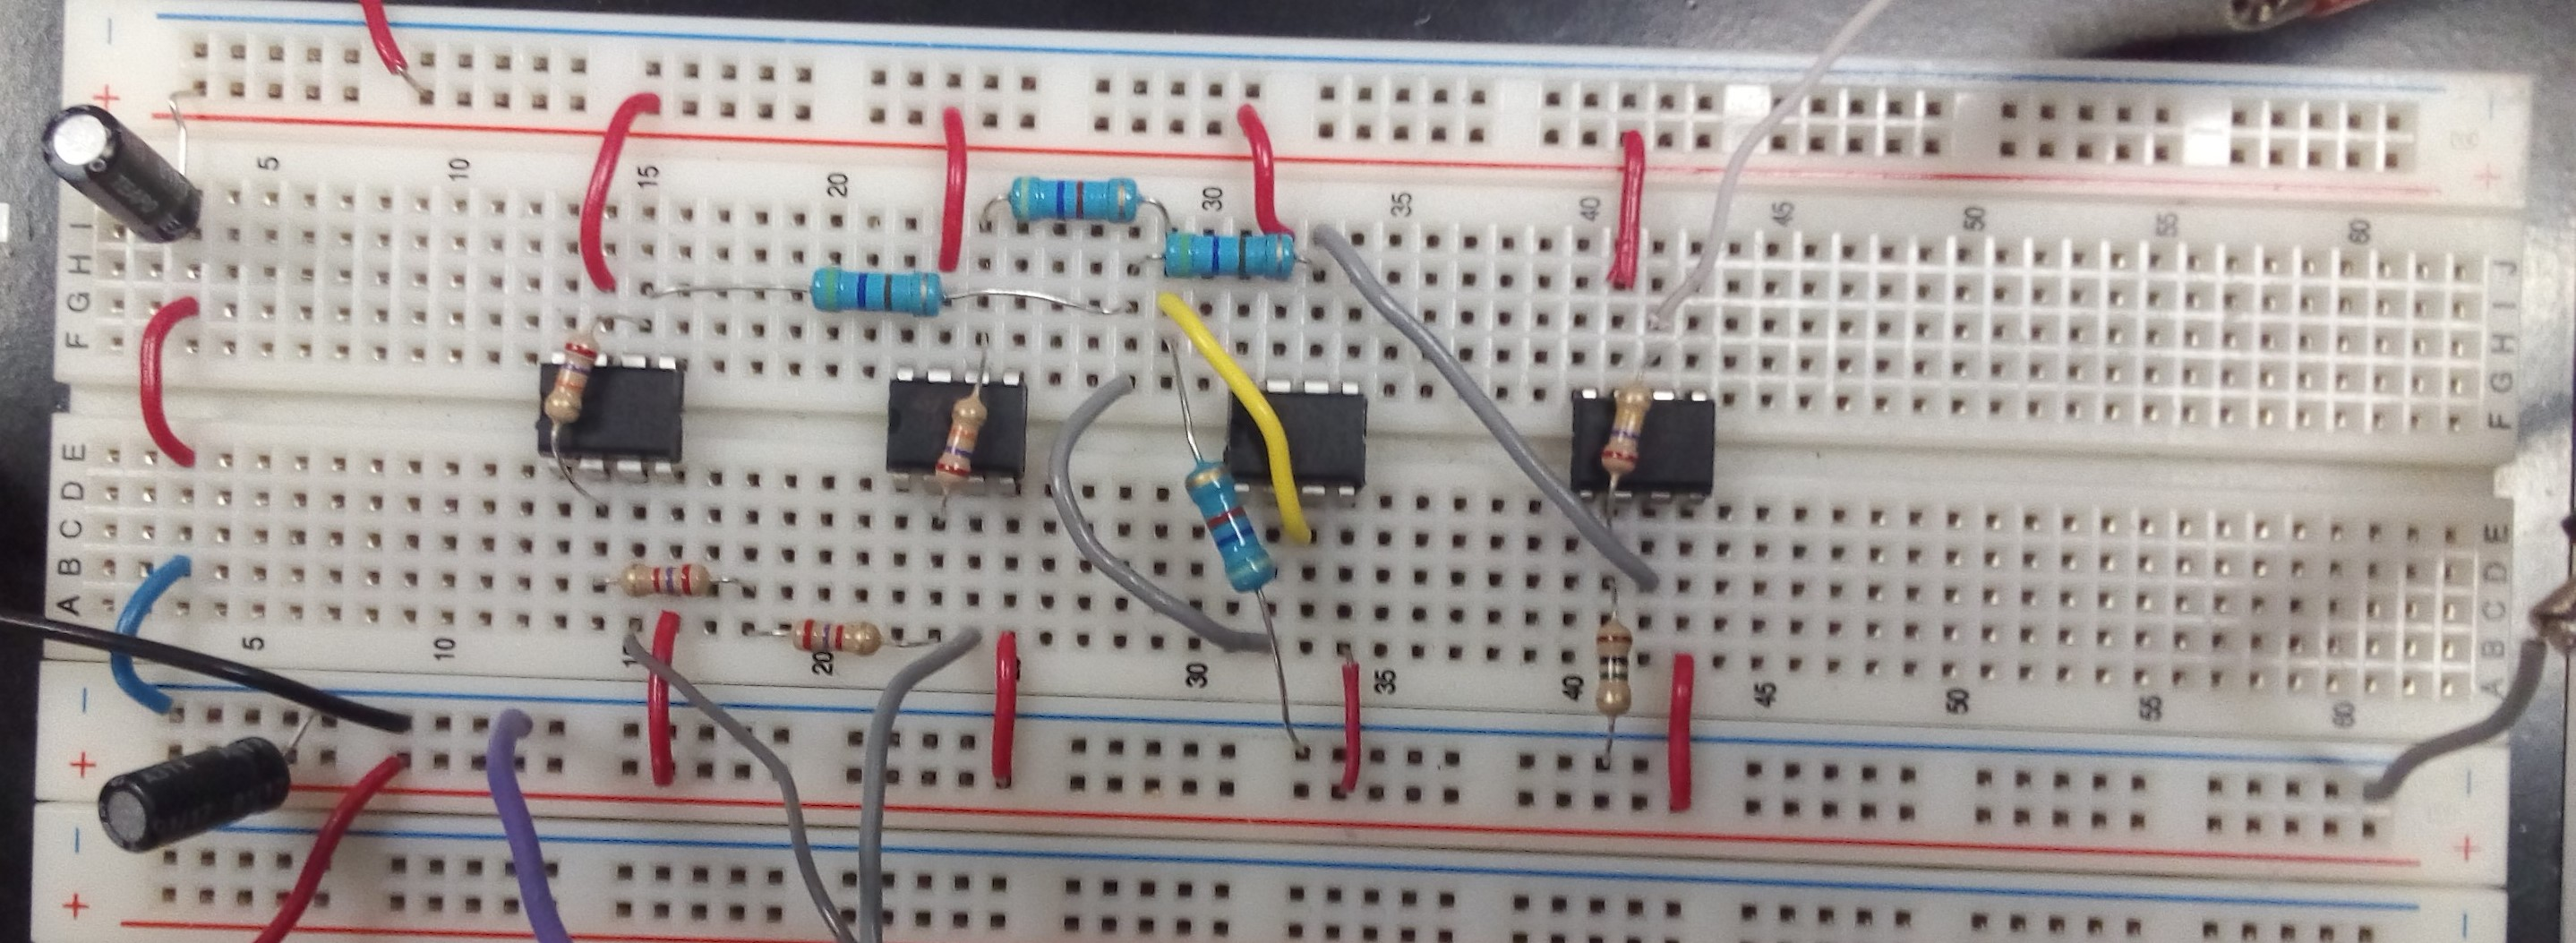
\includegraphics[width=\textwidth]{Practica3/images/circuito1.jpg}
    \end{figure} 
	\subsubsection{Proceso de prueba}
	\textbf{Prueba 1}
	
	Aplicar una señal senoidal desde el generador de funciones de 20 mV a 200 Hz, sin offset, a la entrada del Electrodo 1. Enviar la entrada del Electrodo 2 a tierra.
	
	Posteriormente, medir esta señal de entrada y la salida en $Vo_{1}$ con el osciloscopio.
	
	\textbf{Parámetros de medición (Vpp)}
            \begin{multicols}{2}
                \begin{itemize}
                    \item[\checkmark] \textbf{Amplitud máxima de entrada: 68 mV}
                    \item[\checkmark] \textbf{Amplitud máxima de salida: 472 mV}
                    \item[\checkmark] \textbf{Base de tiempo: 2.5 ms}
            \columnbreak
                    \item[\checkmark] \textbf{Volts por división: 100 mV}
                    \item[\checkmark] \textbf{Acoplamiento: Corriente Continua}
                \end{itemize}
            \end{multicols}
            
            \textbf{Nota:} La señal amarilla (Canal 1) es la señal del que sale del generador de funciones y la azul (Canal 2) la que sale de $Vo_{1}$
            
	        % PONER FOTO DE LA MEDICIÓN PURA, ES DECIR DIRECTAMENTE AL OSCILOSCOPIO
	        \begin{figure}[h!]
                \centering
                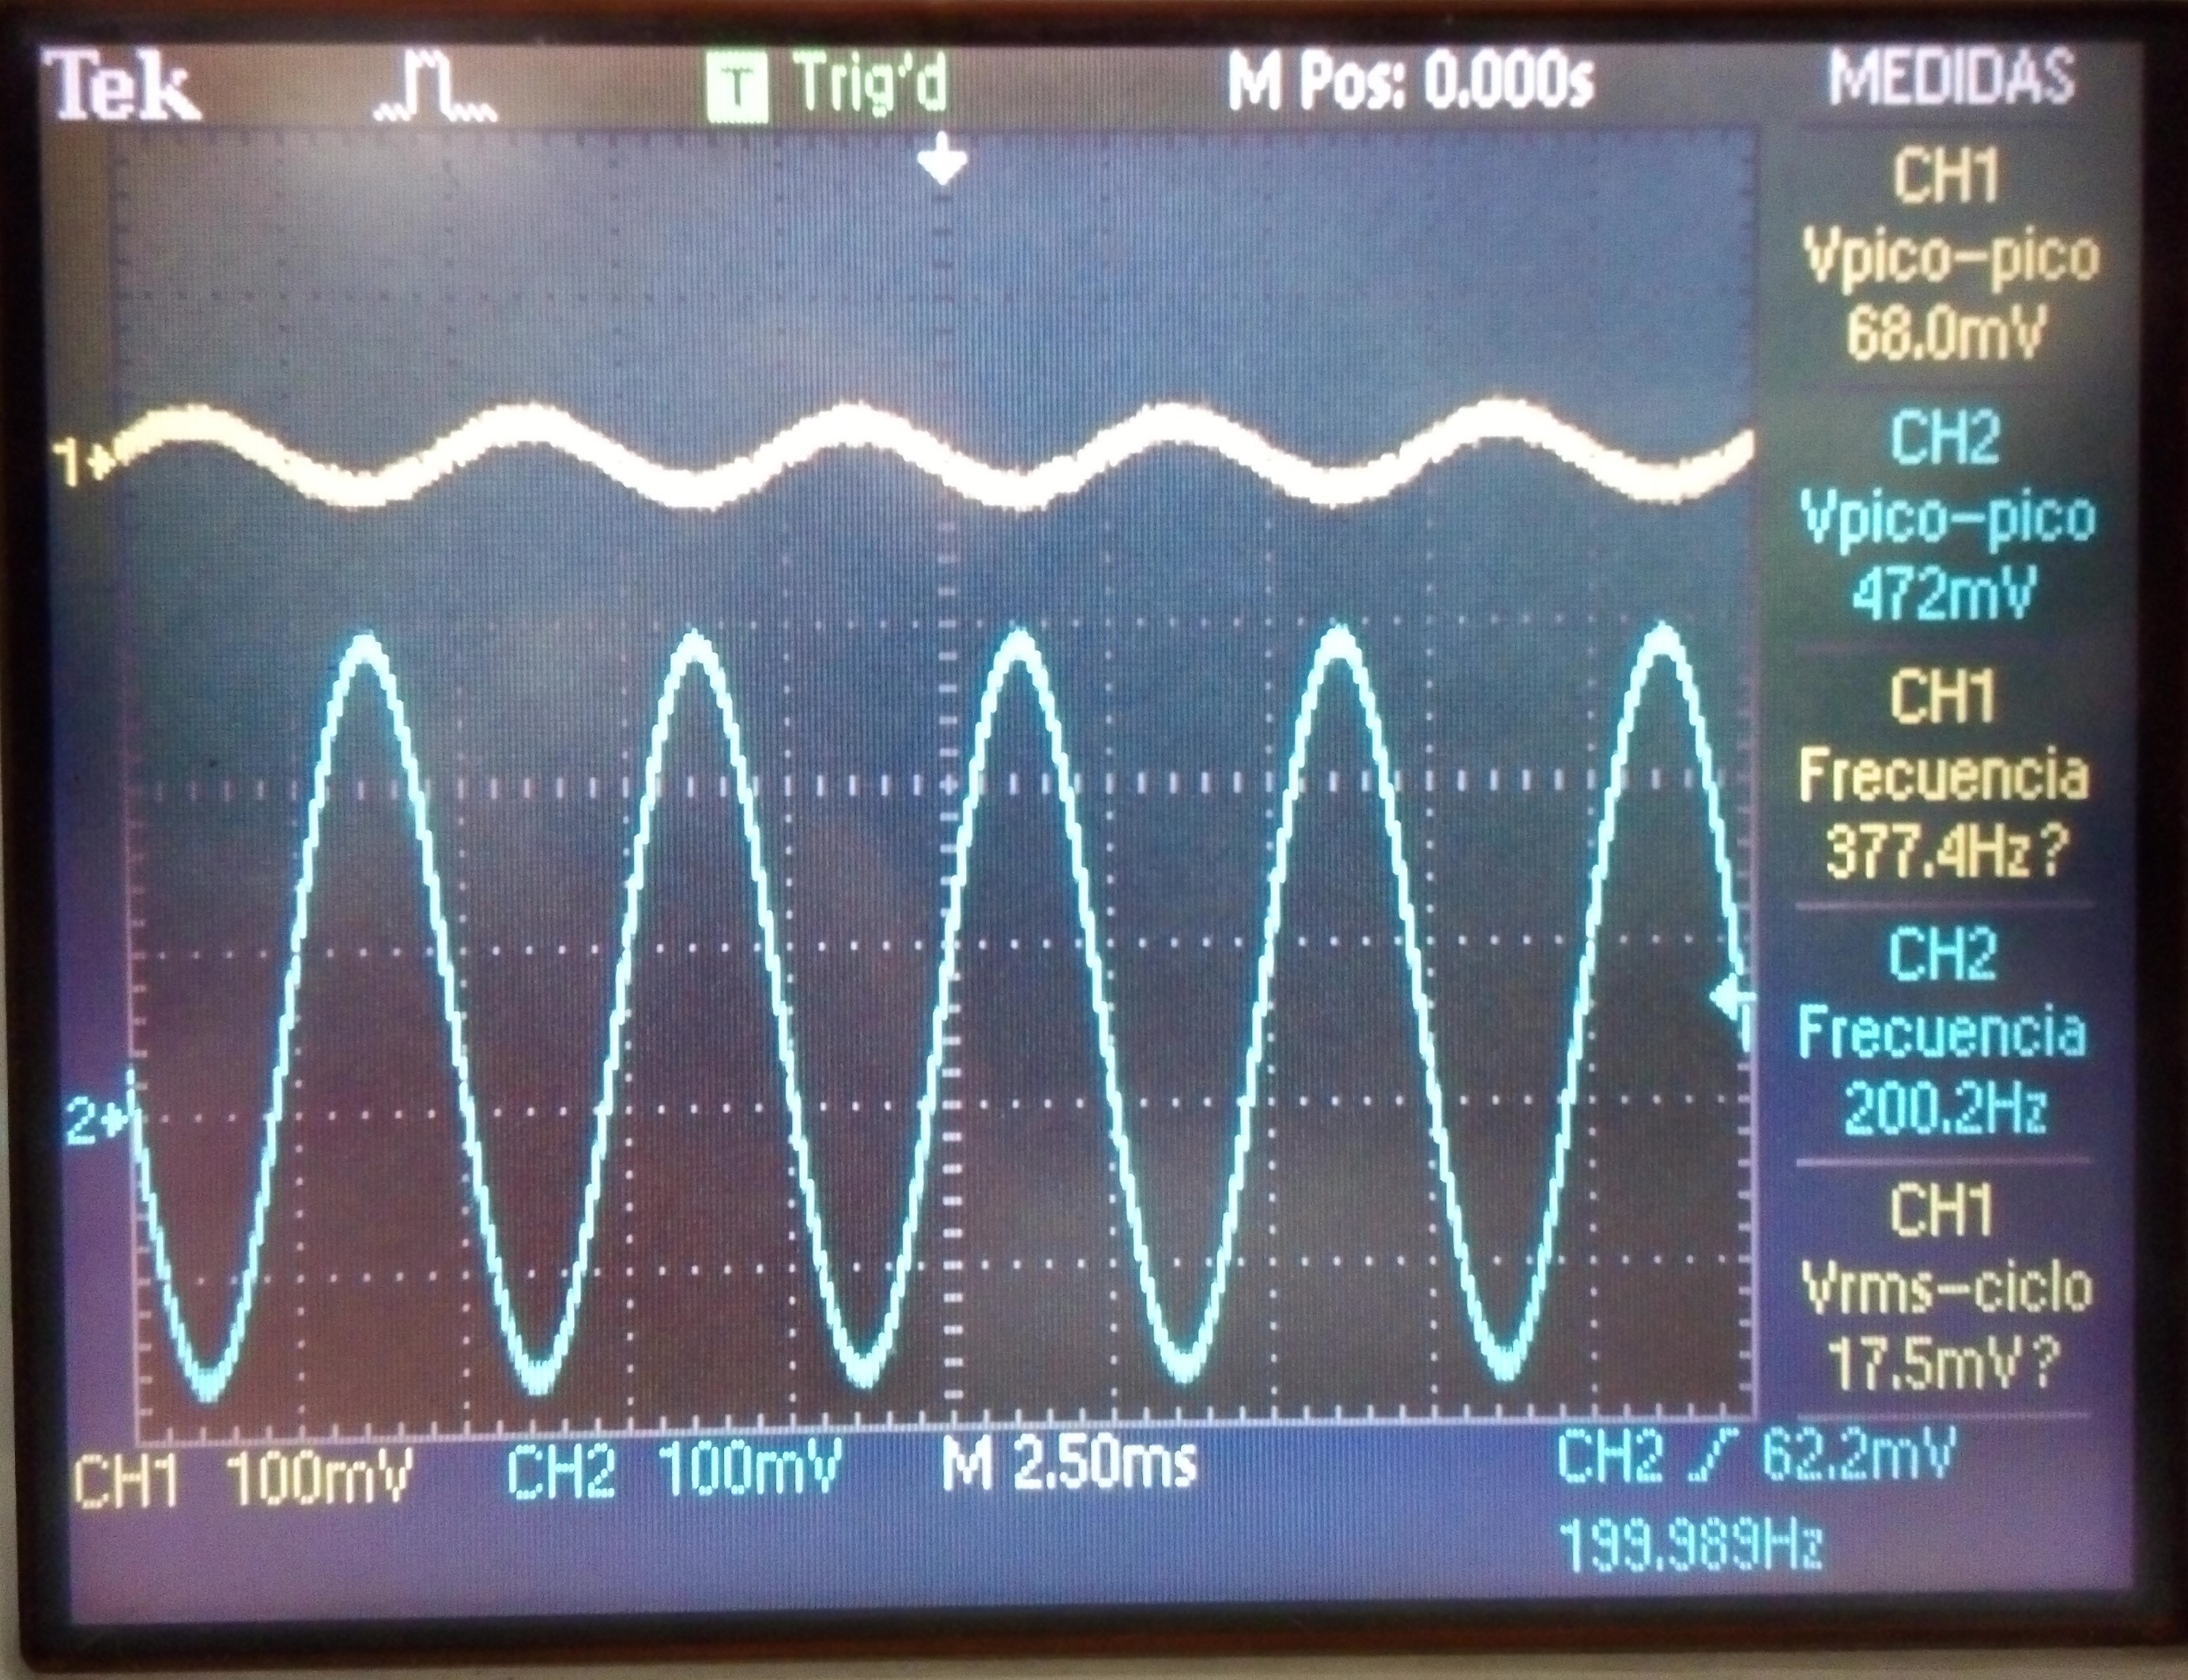
\includegraphics[width=0.7\textwidth]{Practica3/images/prueba1_2.jpg}
            \end{figure} 
            
            La señal del generador de funciones que entra en el Electrodo 1 tiene un voltaje muy pequeño, además de que esta llena de ruido. Podemos notar que en la salida esta señal esta amplificada y tiene una ganancia igual a 6.94, además de que sale filtrada y fina, es decir, sin picos altos ni ruido.
            
            Otra observación importante es que la señal resultante es inversa a la de entrada. La parte inversora del circuito funciona correctamente.
	
	\newpage
	\textbf{Prueba 2}
	
	Aplicar una señal senoidal desde el generador de funciones de 20 mV a 200 Hz, sin offset, a la entrada del Electrodo 2. Enviar la entrada del Electrodo 1 a tierra.
	
	Posteriormente, medir esta señal de entrada y la salida en $Vo_{1}$ con el osciloscopio.
	
	\textbf{Parámetros de medición (Vpp)}
            \begin{multicols}{2}
                \begin{itemize}
                    \item[\checkmark] \textbf{Amplitud máxima de entrada: 68 mV}
                    \item[\checkmark] \textbf{Amplitud máxima de salida: 472 mV}
                    \item[\checkmark] \textbf{Base de tiempo: 2.5 ms}
            \columnbreak
                    \item[\checkmark] \textbf{Volts por división entrada: 20 mV}
                    \item[\checkmark] \textbf{Volts por división salida: 200 mV}
                    \item[\checkmark] \textbf{Acoplamiento: Corriente Continua}
                \end{itemize}
            \end{multicols}
            
            \textbf{Nota:} La señal amarilla (Canal 1) es la señal del que sale del generador de funciones y la azul (Canal 2) la que sale de $Vo_{1}$
            
	        % PONER FOTO DE LA MEDICIÓN PURA, ES DECIR DIRECTAMENTE AL OSCILOSCOPIO
	        \begin{figure}[h!]
                \centering
                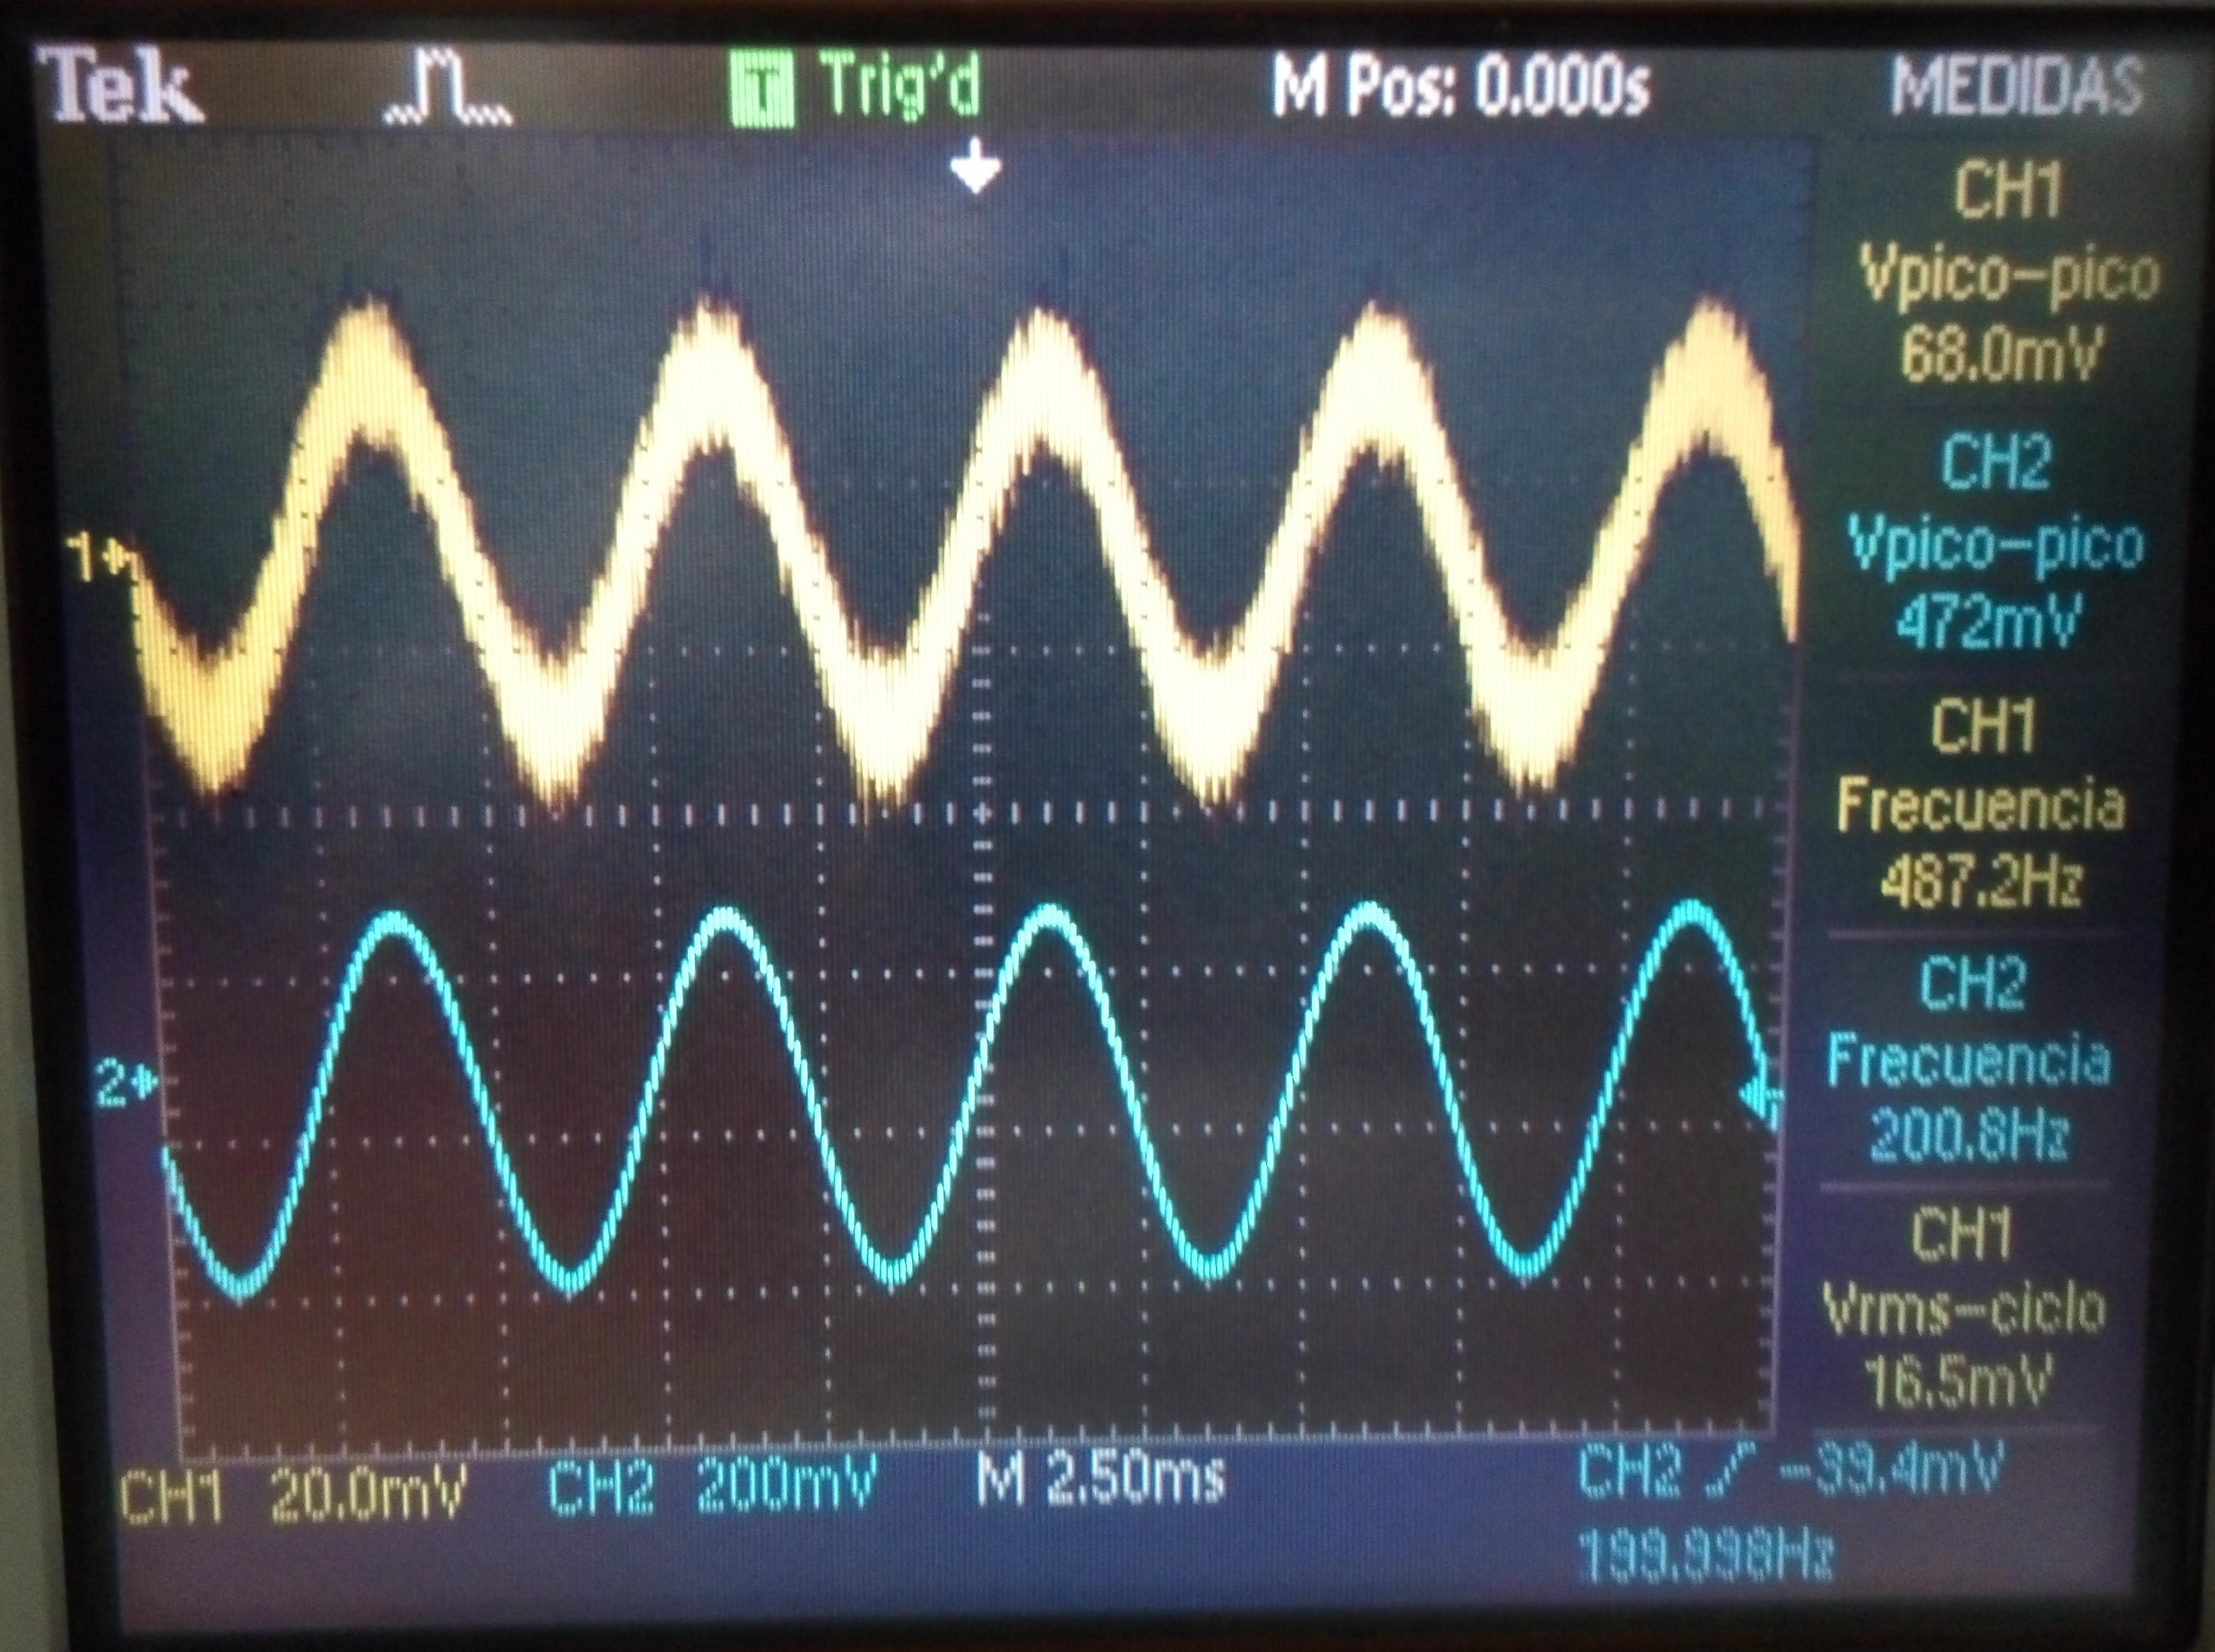
\includegraphics[width=0.7\textwidth]{Practica3/images/prueba2_3.jpg}
            \end{figure} 
            
            La señal del generador de funciones que entra en el Electrodo 2 tiene un voltaje muy pequeño, además de que esta llena de ruido. Similar a la prueba anterior, en la salida esta señal esta amplificada y tiene una ganancia igual a 6.94, además de que sale filtrada y fina, es decir, sin picos altos ni ruido.
            
            Otra observación importante es que la señal resultante es no inversa a la de entrada, por lo que señal sale completamente igual, filtrada y amplificada. La parte no inversora del circuito funciona correctamente.
	\newpage
	\textbf{Prueba 3}
	
	Aplicar una señal senoidal desde el generador de funciones de 20 mV a 200 Hz, sin offset, a la entrada del Electrodo 2 y a la entrada del Electrodo 1. 
	
	Posteriormente, medir esta señal de entrada y la salida en $Vo_{2}$ con el osciloscopio.
	
	
	
	\textbf{Parámetros de medición (Vpp)}
            \begin{multicols}{2}
                \begin{itemize}
                    \item[\checkmark] \textbf{Amplitud máxima de entrada: 0 V}
                    \item[\checkmark] \textbf{Amplitud máxima de salida: 20 mV}
                    \item[\checkmark] \textbf{Base de tiempo: 250 ms}
            \columnbreak
                    \item[\checkmark] \textbf{Volts por división: 100 mV}
                    \item[\checkmark] \textbf{Acoplamiento: Corriente Continua}
                \end{itemize}
            \end{multicols}
            
            \textbf{Nota:} La señal amarilla (Canal 1) es la señal del que sale del generador de funciones y la azul (Canal 2) la que sale de $Vo_{2}$
            
            % PONER FOTO DE LA MEDICIÓN PURA, ES DECIR DIRECTAMENTE AL OSCILOSCOPIO
	        \begin{figure}[h!]
                \centering
                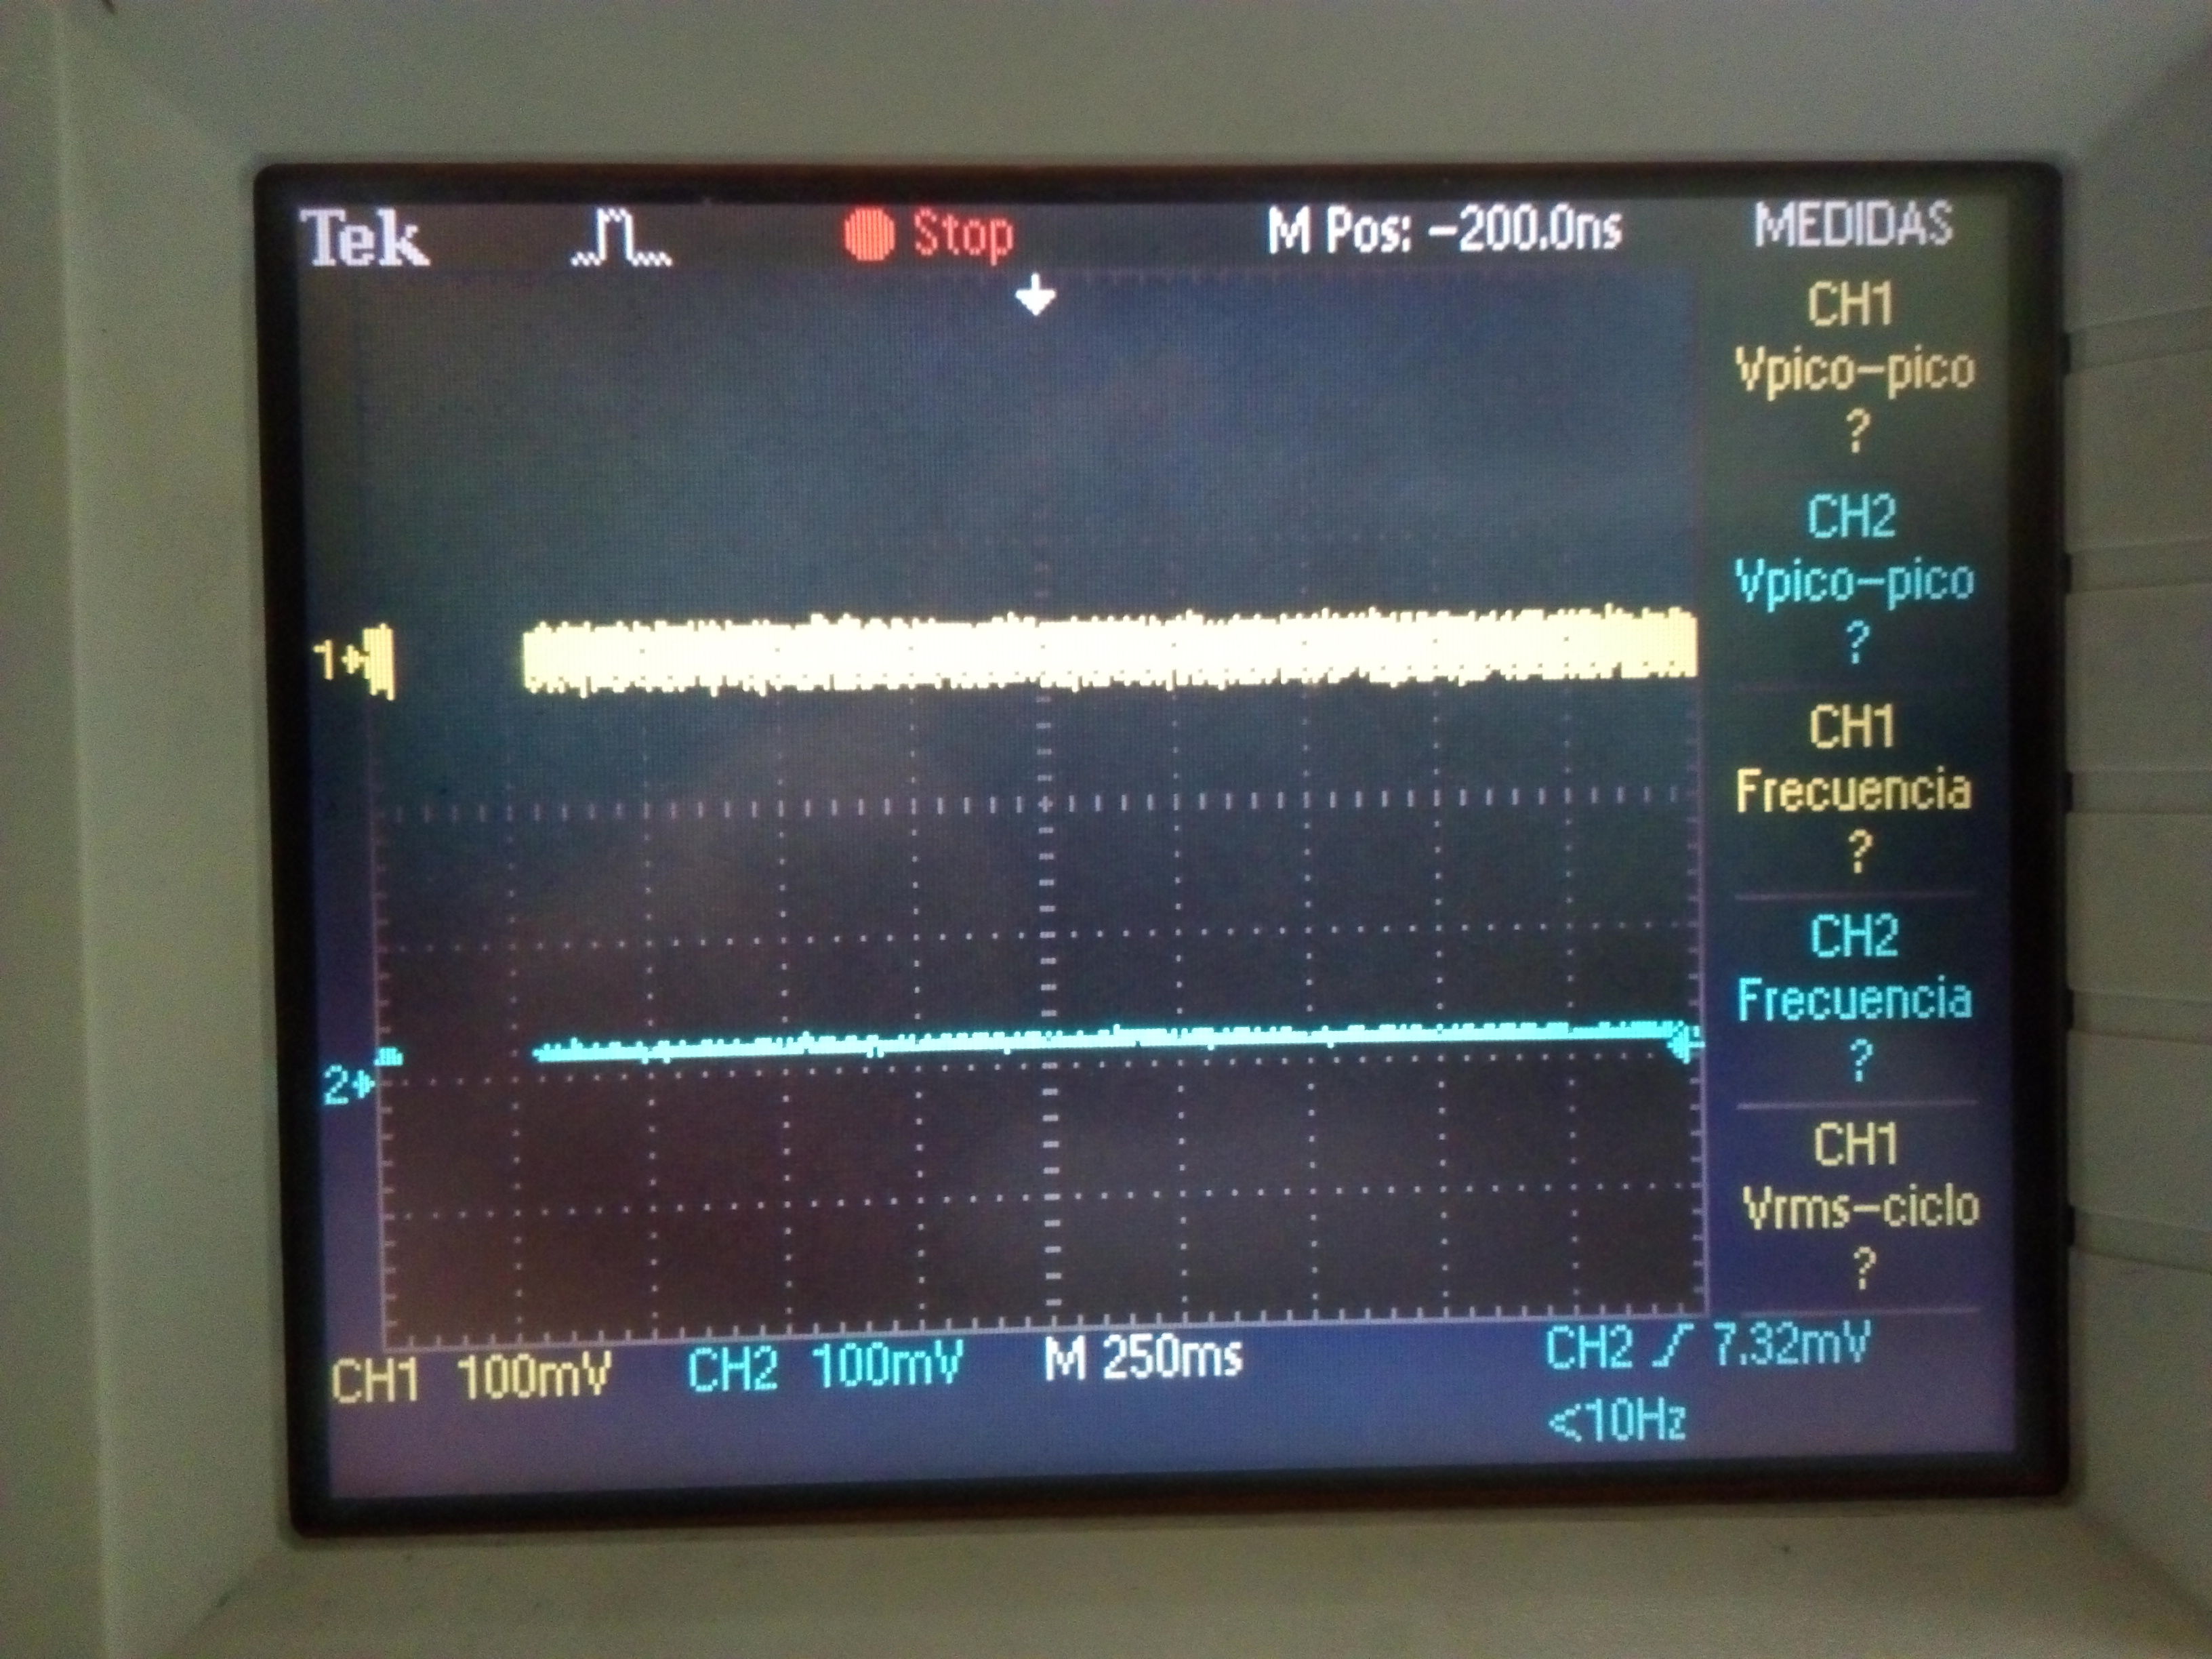
\includegraphics[width=0.7\textwidth]{Practica3/images/prueba3_4.jpg}
            \end{figure} 
            
            Como se observa en la prueba 2, la señal del canal 1 y la señal del canal 2, sale la misma señal, por lo que, para la prueba 3, como se van a restar dichas señales, debe salir una señal lineal. 
            
            Lo anterior es para cuando se encuentra estable la entrada del electrodo 2, para que cuando se aplique fuerza, se pueda mostrar la señal que genera dicho esfuerzo. 
            
            Por otro lado, esta prueba nos indica el error que tendrán nuestras mediciones, ya que al igual que las señales mioelectricas puras que nos interesan, este también se amplificará. Este error es mínimo, pero existente, ya que la señal no esta posicionada exactamente en los 0 V, sino que es de aproximadamente 20 mV ya amplificada.
	
	\newpage
	\subsubsection{Medición de la señal muscular}
	Una vez concluidas las pruebas que muestran la correcta configuración del circuito, es momento de medir la señal muscular.
	
	Se deben colocar tres electrodos de 6 x 3 cm hechos a partir de placas fenólicas de cobre en el brazo del sujeto de prueba como se muestra a continuación:
	
	% PONER FOTO DEL BRAZO CON LOS ELECTRODOS
	        \begin{figure}[h!]
                \centering
                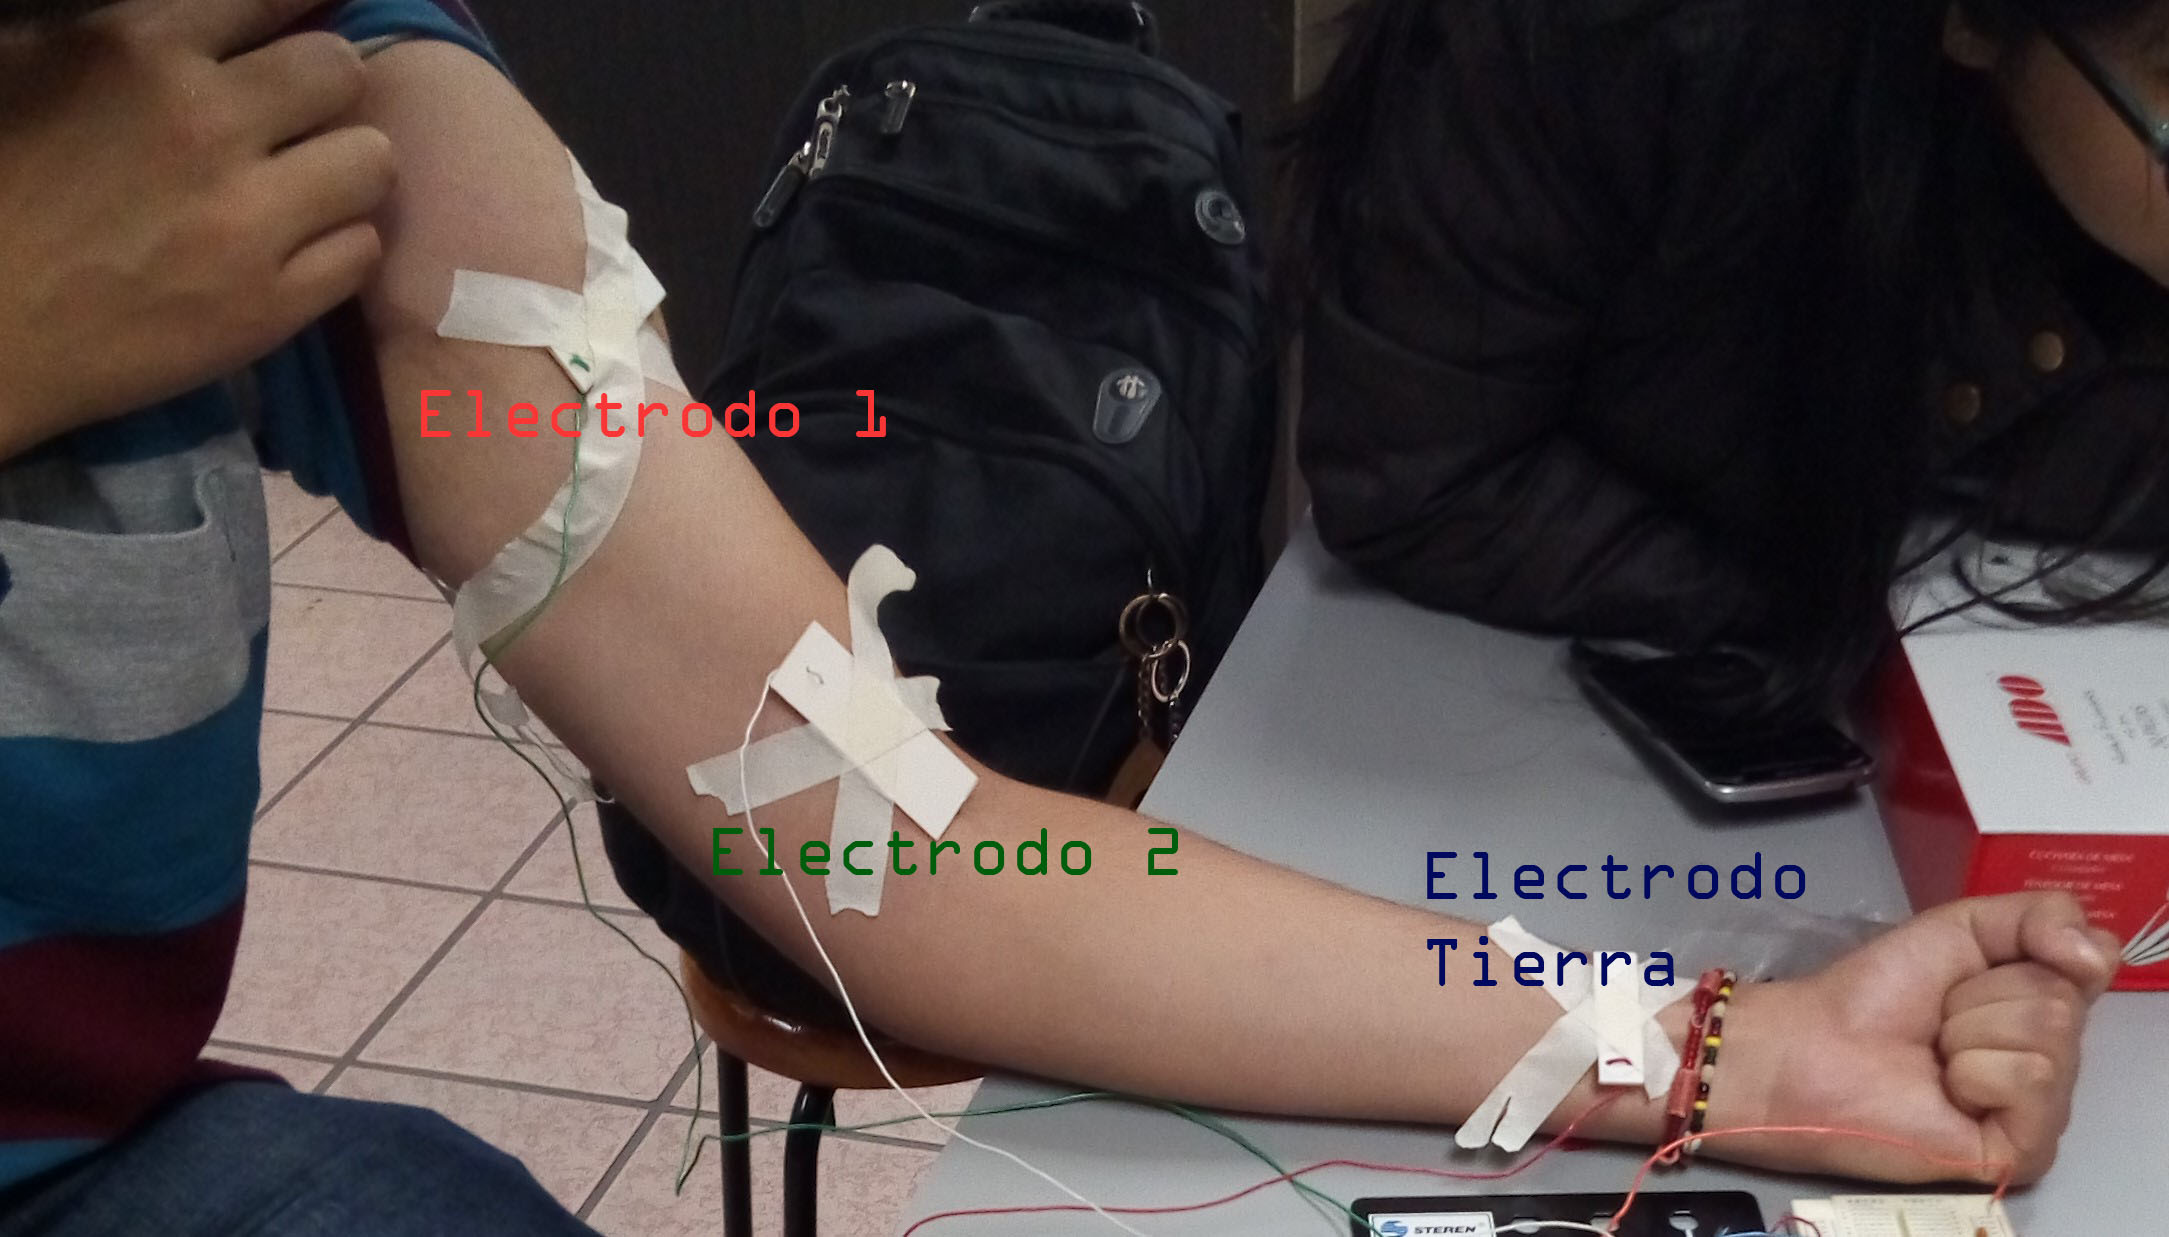
\includegraphics[width=0.85\textwidth]{Practica3/images/electrobrazo.jpg}
            \end{figure}
    
    Ya con los electrodos sujetados al brazo, la medición constaba en contraer los músculos del brazo por un corto periodo de tiempo, aplicando fuerza y manteniéndolo firme tratando no hacerlo temblar (pues enviamos señales no deseadas al circuito) de la forma que se presenta en la imagen superior, y posteriormente relajarlo para visualizar el cambio de señal en el osciloscopio.
    
    A continuación se muestra una de estas señales obtenidas al medir en $Vo_{1}$:
    
    \textbf{Parámetros de medición (Vpp)}
            \begin{multicols}{2}
                \begin{itemize}
                    \item[\checkmark] \textbf{Amplitud máxima (sin picos): 232 mV}
                    \item[\checkmark] \textbf{Base de tiempo: 1 s}
            \columnbreak
                    \item[\checkmark] \textbf{Volts por división: 50 mV}
                    \item[\checkmark] \textbf{Acoplamiento: Corriente Alterna}
                \end{itemize}
            \end{multicols}
            
            Cuando el músculo esta relajado, el osciloscopio no detecta ninguna señal con alta amplitud, por lo que solo despliega una ligera señal de aproximadamente 16 mV, debido a un ruido que entra en el circuito.
    \newpage
    % PONER FOTO SEÑAL EN VO1
	        \begin{figure}[h!]
                \centering
                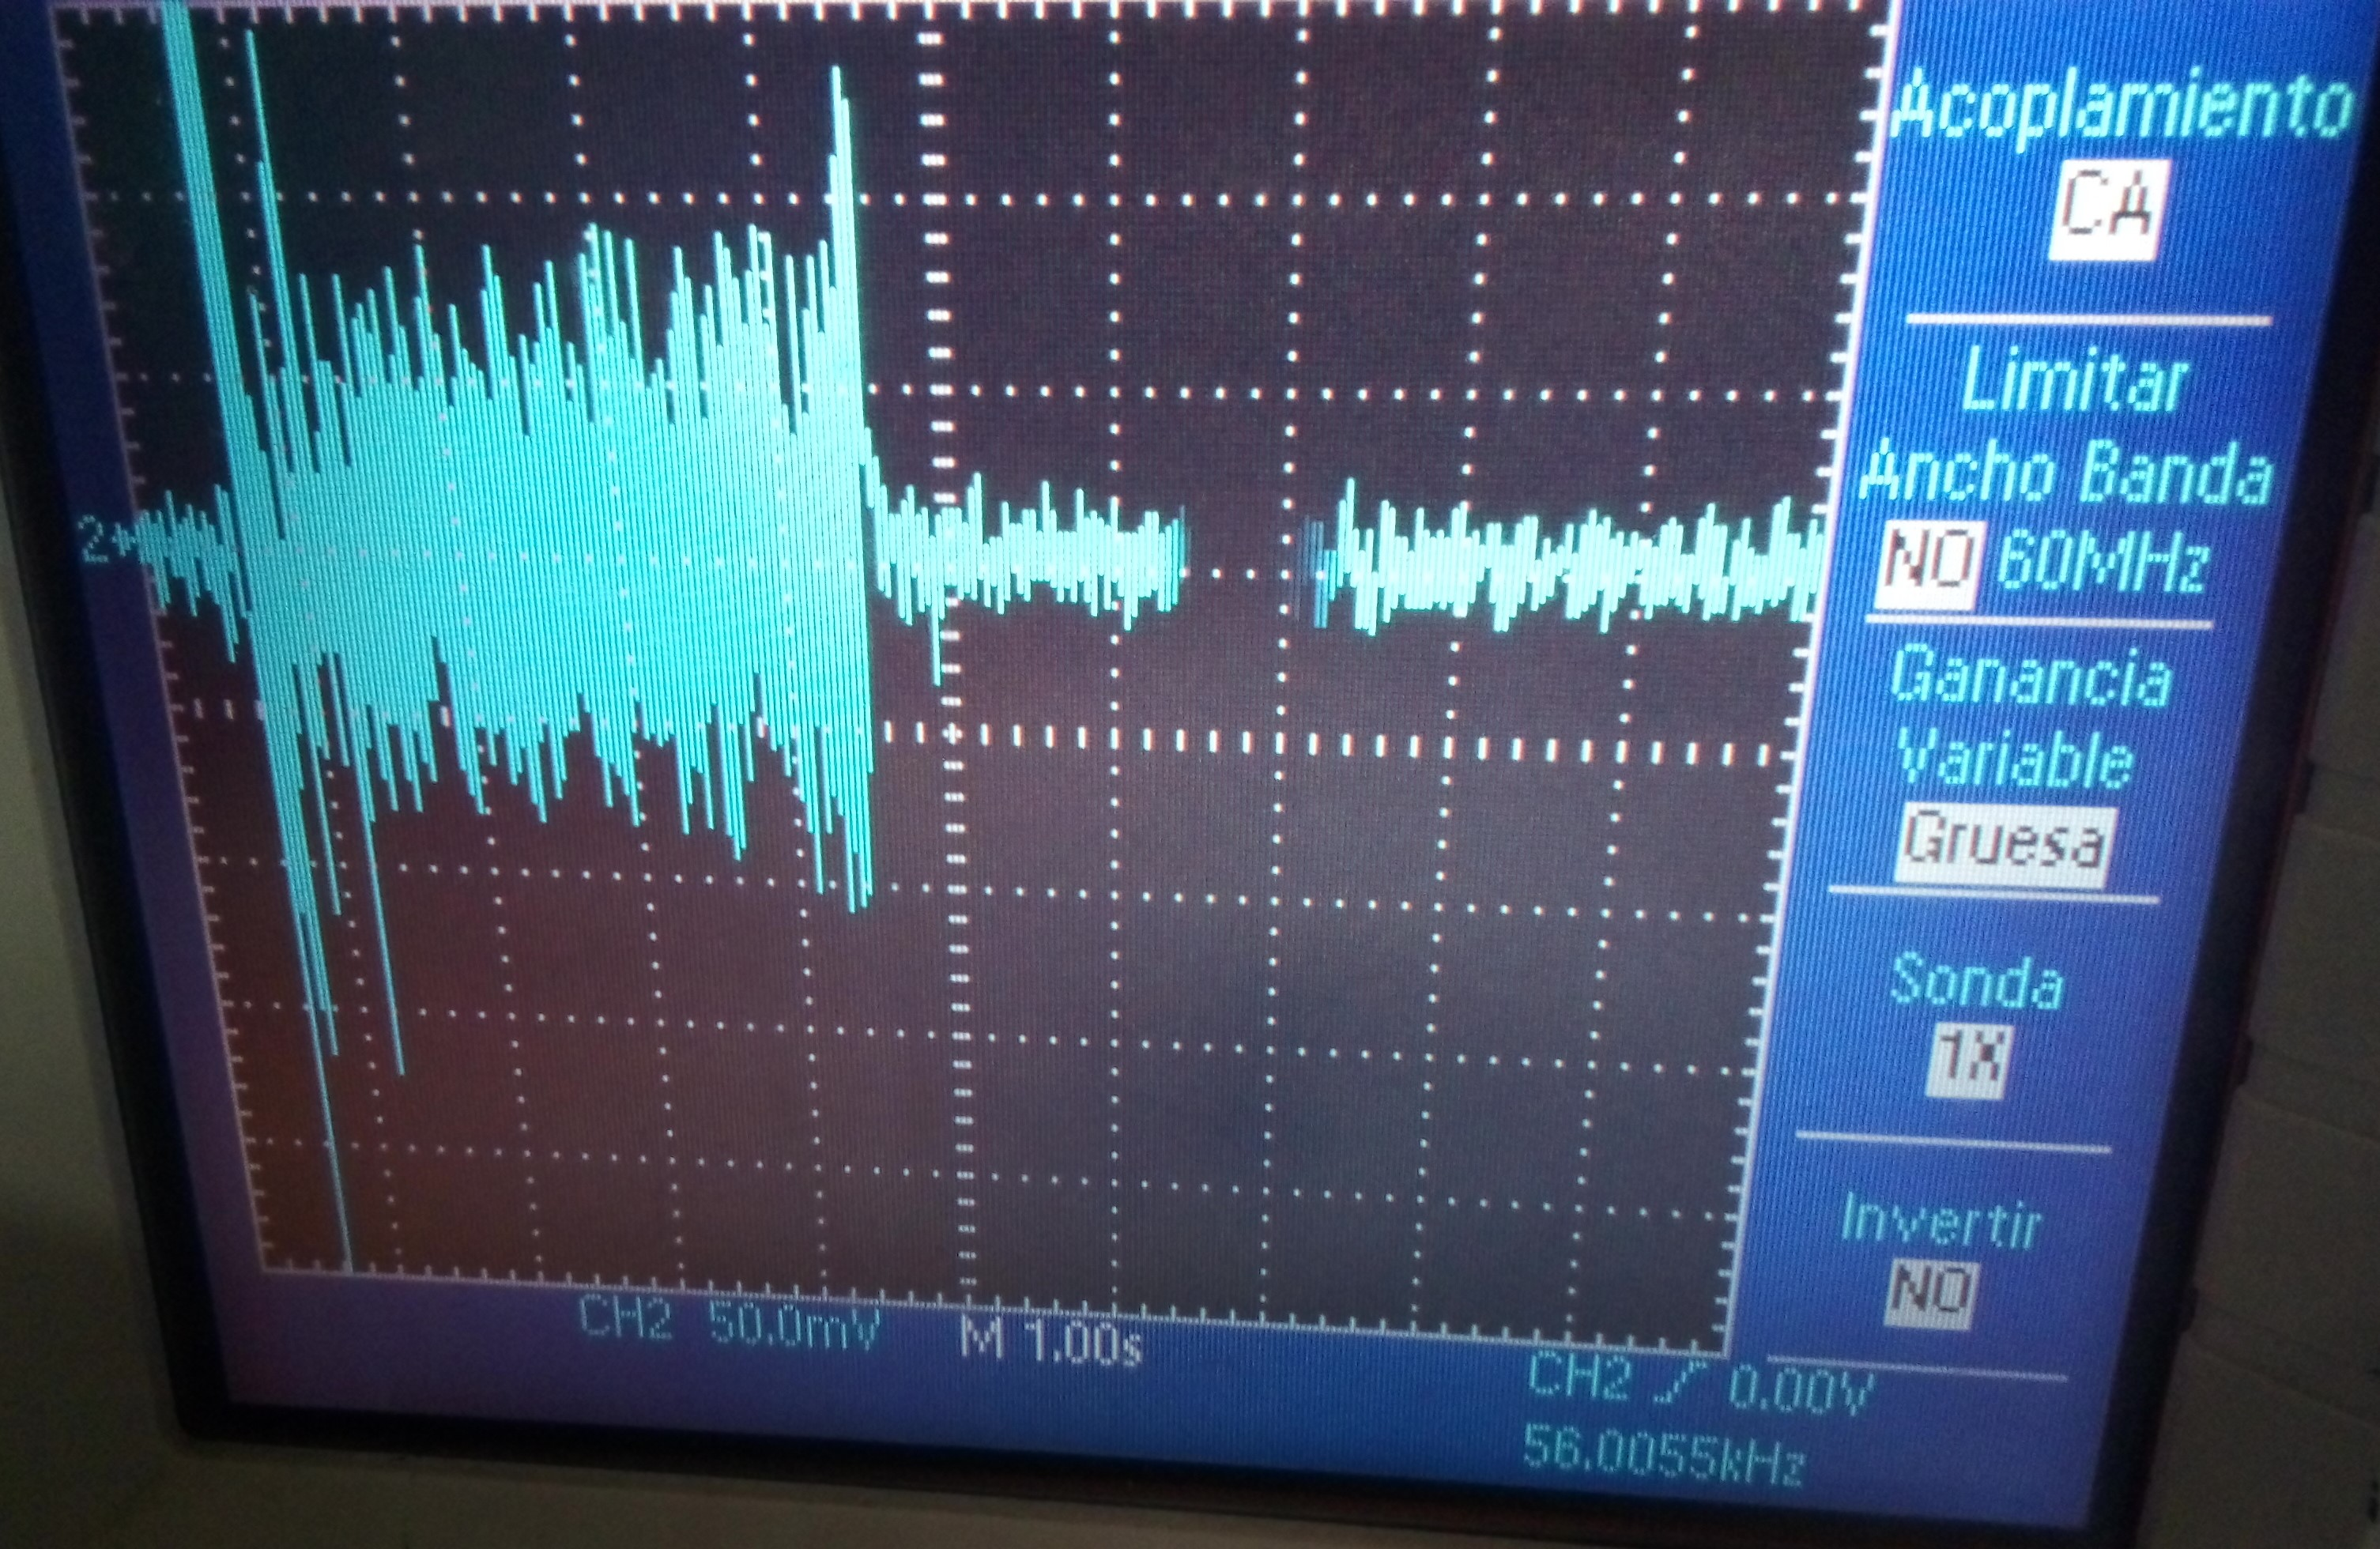
\includegraphics[width=0.65\textwidth]{Practica3/images/senalVo1_3.jpg}
            \end{figure}
            
        
        
        Midiendo ahora en $Vo_{2}$:
        
        \textbf{Parámetros de medición (Vpp)}
            \begin{multicols}{2}
                \begin{itemize}
                    \item[\checkmark] \textbf{Amplitud máxima: 800 mV}
                    \item[\checkmark] \textbf{Base de tiempo: 1 s}
            \columnbreak
                    \item[\checkmark] \textbf{Volts por división: 200 mV}
                    \item[\checkmark] \textbf{Acoplamiento: Corriente Alterna}
                \end{itemize}
            \end{multicols}
        
        % PONER FOTO SEÑAL EN VO2
	        \begin{figure}[h!]
                \centering
                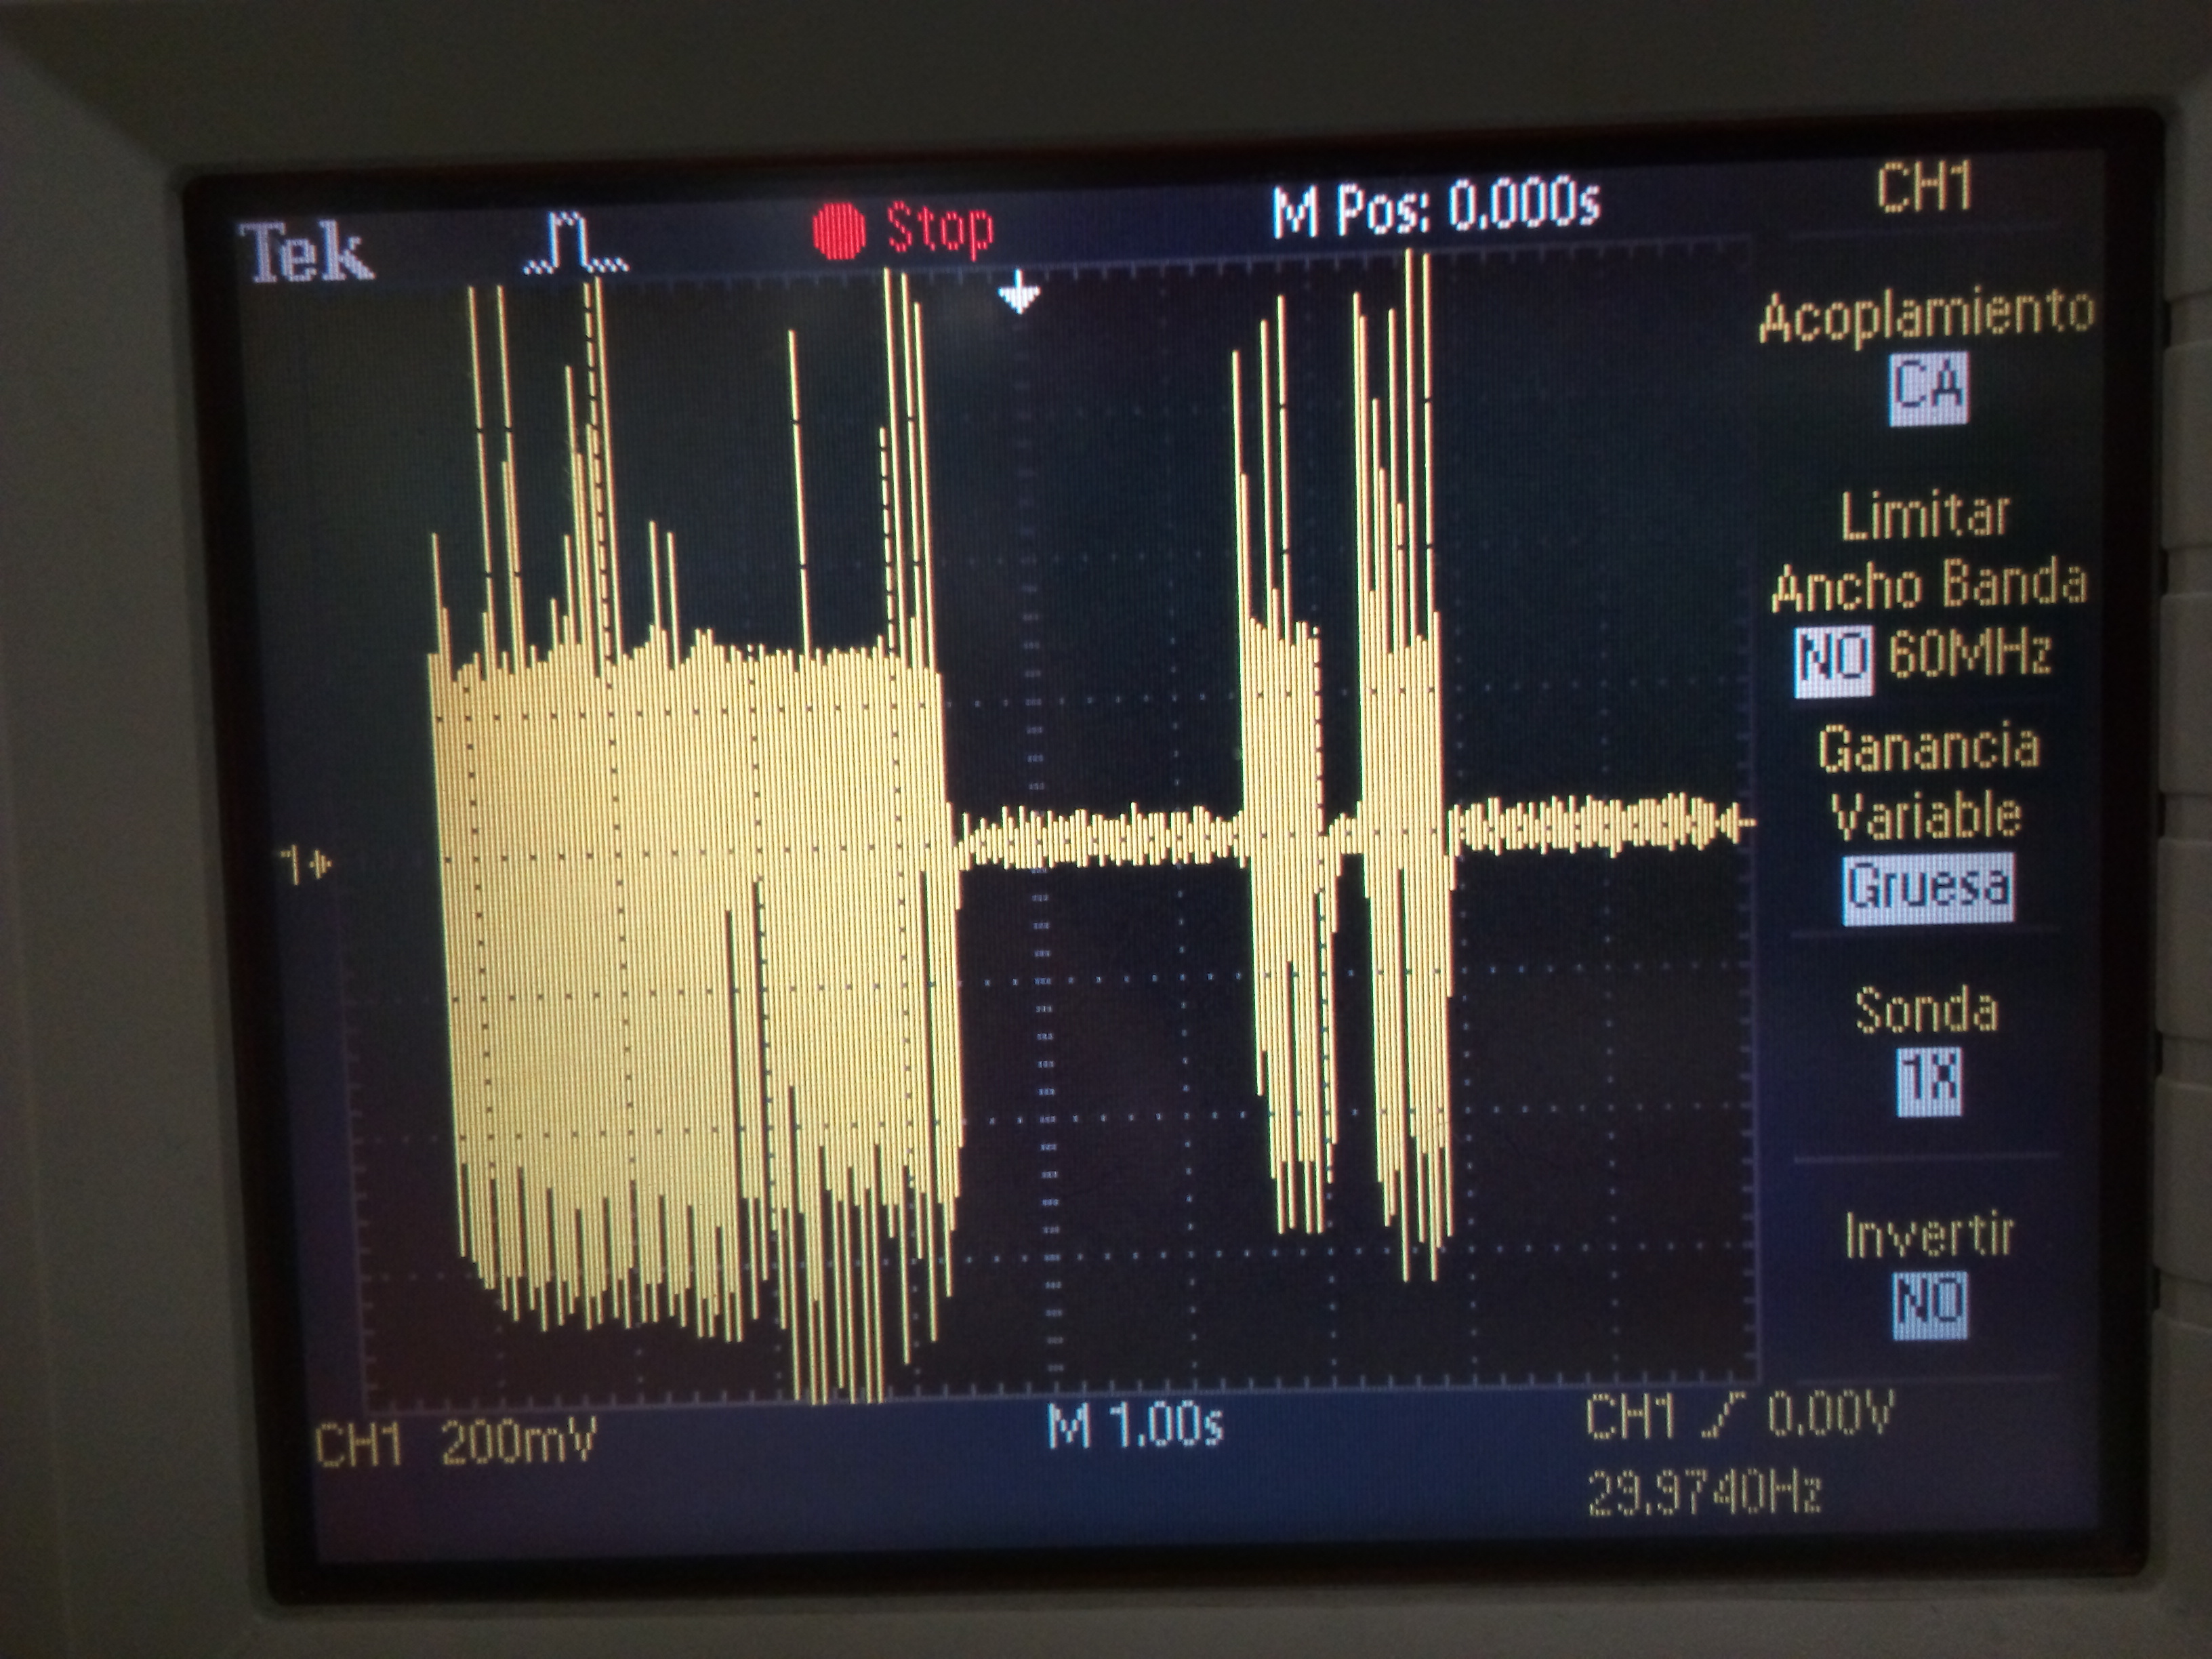
\includegraphics[width=0.65\textwidth]{Practica3/images/senalVo2.jpg}
            \end{figure}
        
        Nos encontramos con que el circuito sí detecta el cambio entre la tensión muscular del brazo al aplicar fuerza o relajarlo, pero la señal no sale amplificada a 10 Vpp como se esperaría, además de aun contener un ligero ruido al relajar el brazo. 
        
        El amplificador de instrumentación no esta devolviendo la diferencia entre las 2 señales que entran en los electrodos de forma correcta, pues si lo hiciera, este ruido sería eliminado.
        
        El problema lo solucionaremos en la siguiente etapa, aplicando un amplificador extra como filtro.

	\subsection{PE 2 - Circuito 2: Filtro}
		\subsubsection{Esquema}
	\begin{figure}[h!]
                \centering
                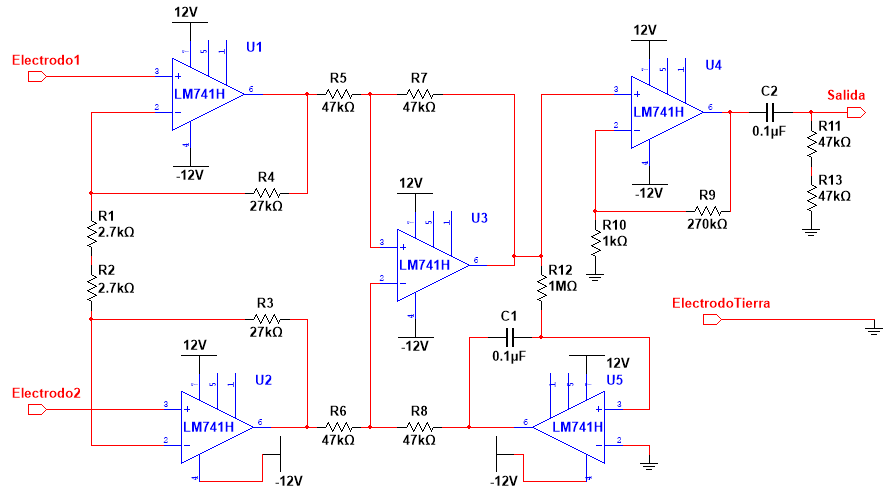
\includegraphics[width=\textwidth]{Practica3/images/ccircuito2.PNG}
    \end{figure} 
	\subsubsection{Circuito cableado}
		\begin{figure}[h!]
                \centering
                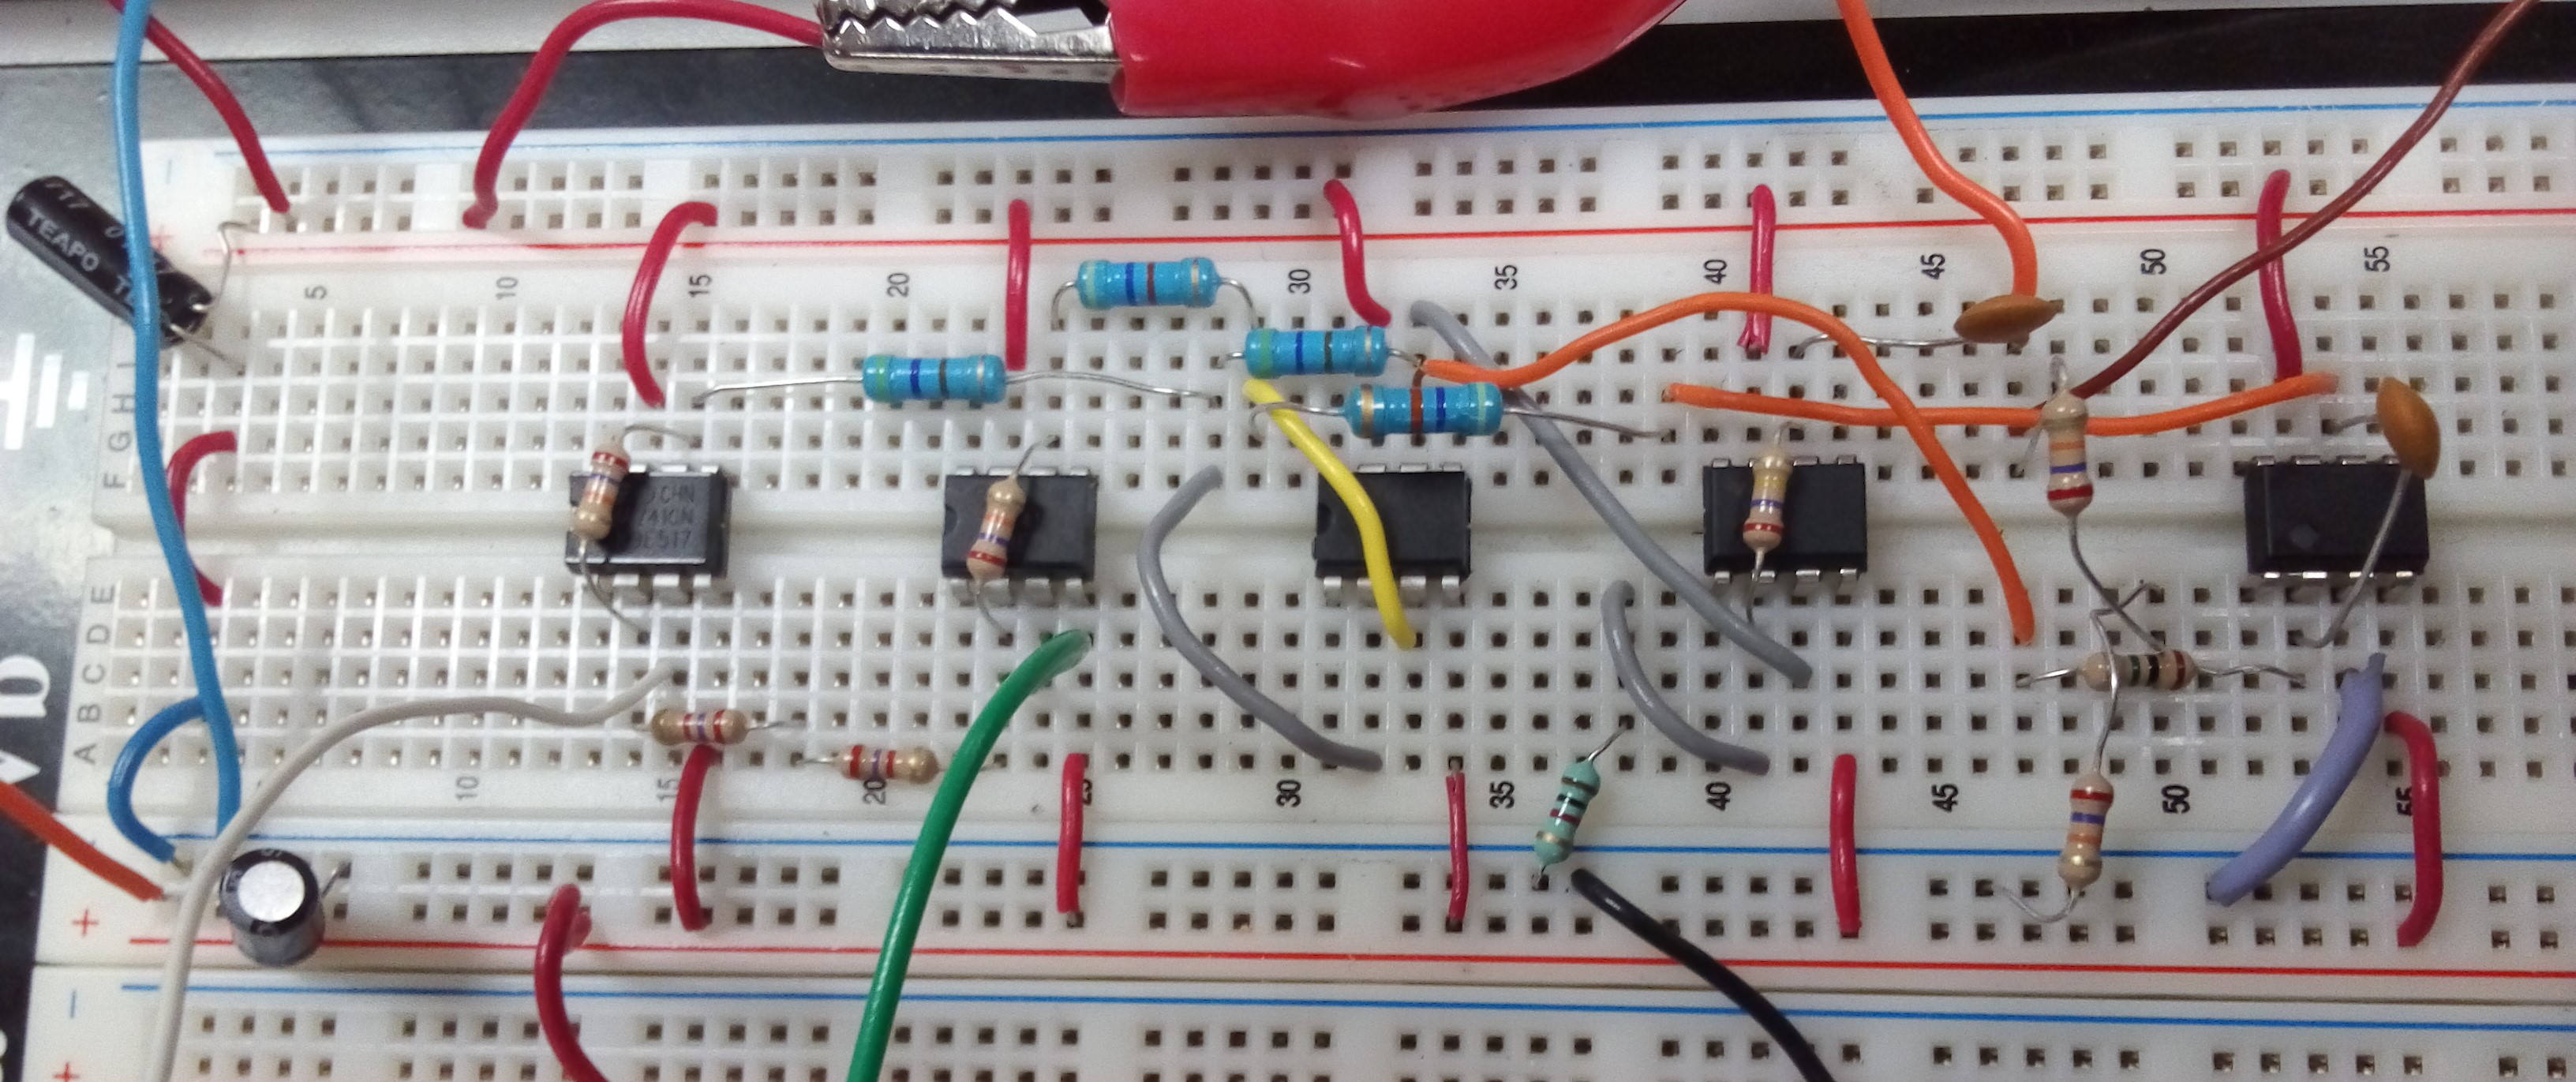
\includegraphics[width=0.95\textwidth]{Practica3/images/circuito2-1.jpg}
    \end{figure} 
    \newpage
	\subsubsection{Medición de la señal muscular}
	Ya que se ha colocado el filtro, es momento de medir nuevamente a señal muscular, esto se hace de manera análoga a la medición anterior. 
	
	\begin{figure}[h!]
                \centering
                \includegraphics[width=0.6\textwidth]{Practica3/images/m_filtro.jpg}
            \end{figure}

        Ahora, como ya está filtrada la señal, cuando el músculo está relajada, debe salir una señal estable, y cuando se ejerza fuerza, deberá mostrar la señal de esta acción. Todas las mediciones se realizaron en la salida del circuito, o $Vo_{2}$.
        
        \textbf{Parámetros de medición (Vpp)}
            \begin{multicols}{2}
                \begin{itemize}
                    \item[\checkmark] \textbf{Amplitud máxima: 6.2 V}
                    \item[\checkmark] \textbf{Base de tiempo: 1 s}
            \columnbreak
                    \item[\checkmark] \textbf{Volts por división: 1 V}
                    \item[\checkmark] \textbf{Acoplamiento: Corriente Alterna}
                \end{itemize}
            \end{multicols}
            \newpage
         
            \begin{figure}[h!]
                \centering
                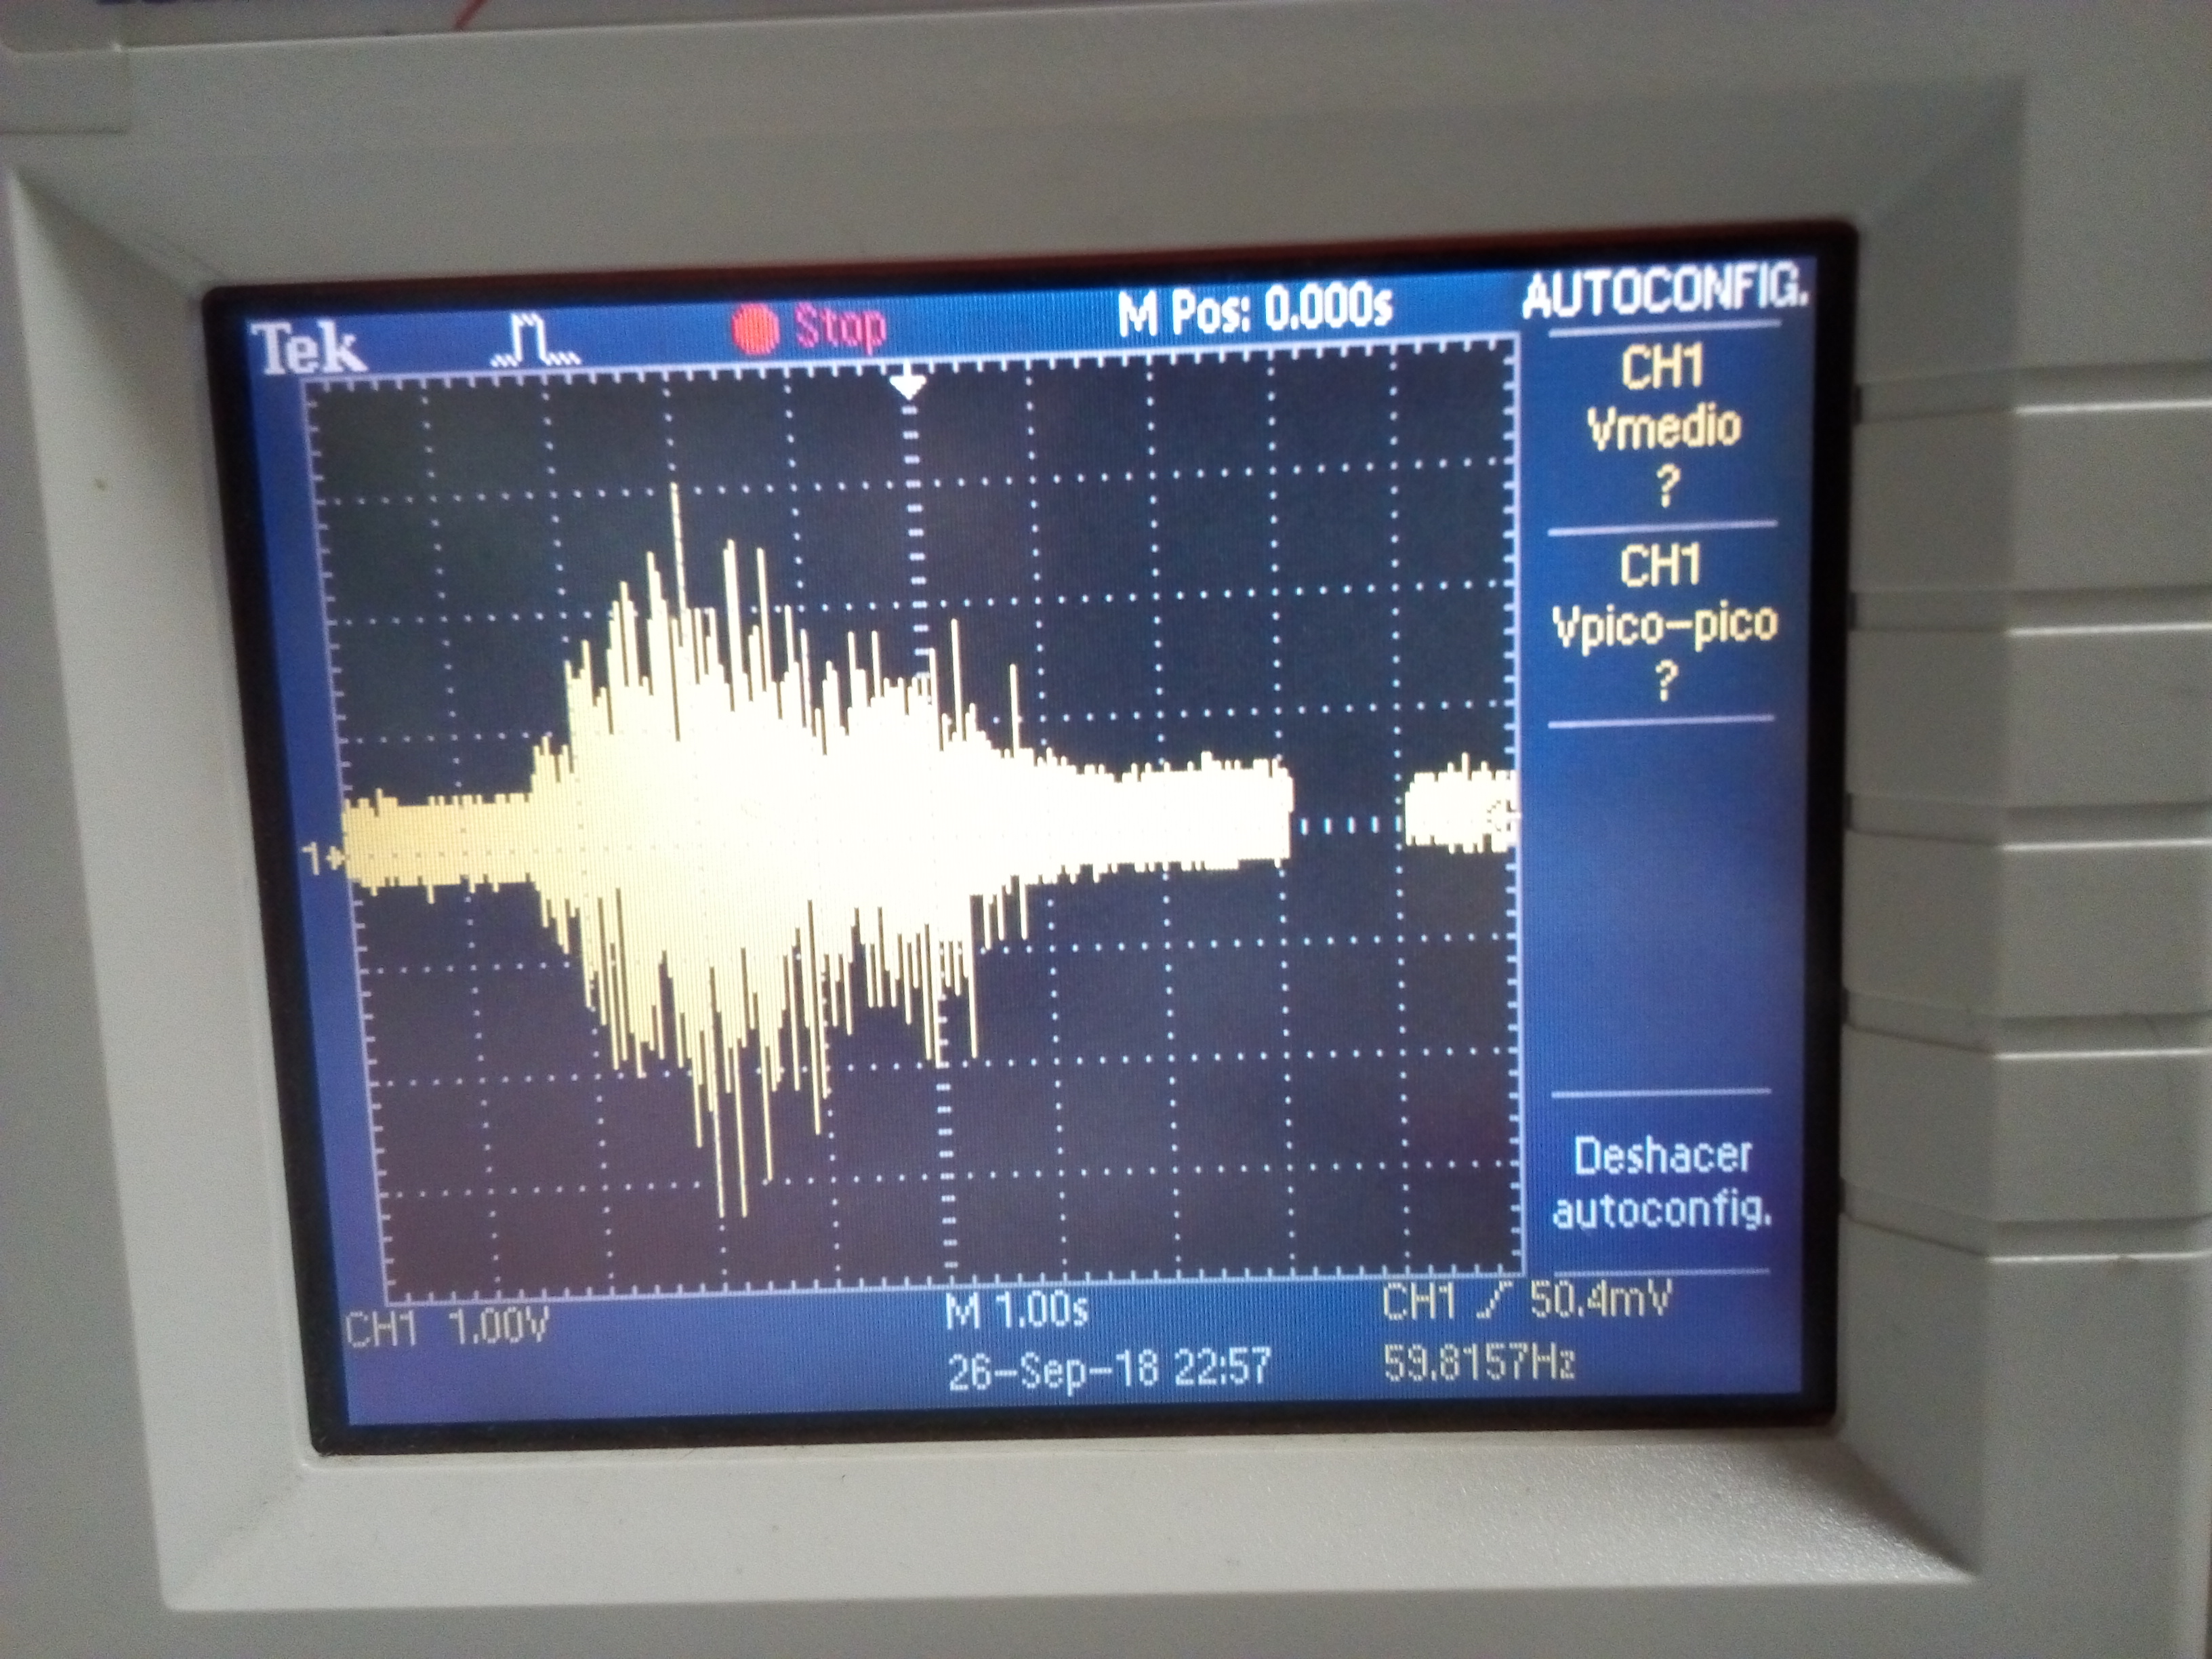
\includegraphics[width=0.75\textwidth]{Practica3/images/filtrada10.jpg}
            \end{figure}
            
            \textbf{Parámetros de medición (Vpp)}
            \begin{multicols}{2}
                \begin{itemize}
                    \item[\checkmark] \textbf{Amplitud máxima: 6.6 V}
                    \item[\checkmark] \textbf{Base de tiempo: 250 ms}
            \columnbreak
                    \item[\checkmark] \textbf{Volts por división: 2 V}
                    \item[\checkmark] \textbf{Acoplamiento: Corriente Alterna}
                \end{itemize}
            \end{multicols}
         
            \begin{figure}[h!]
                \centering
                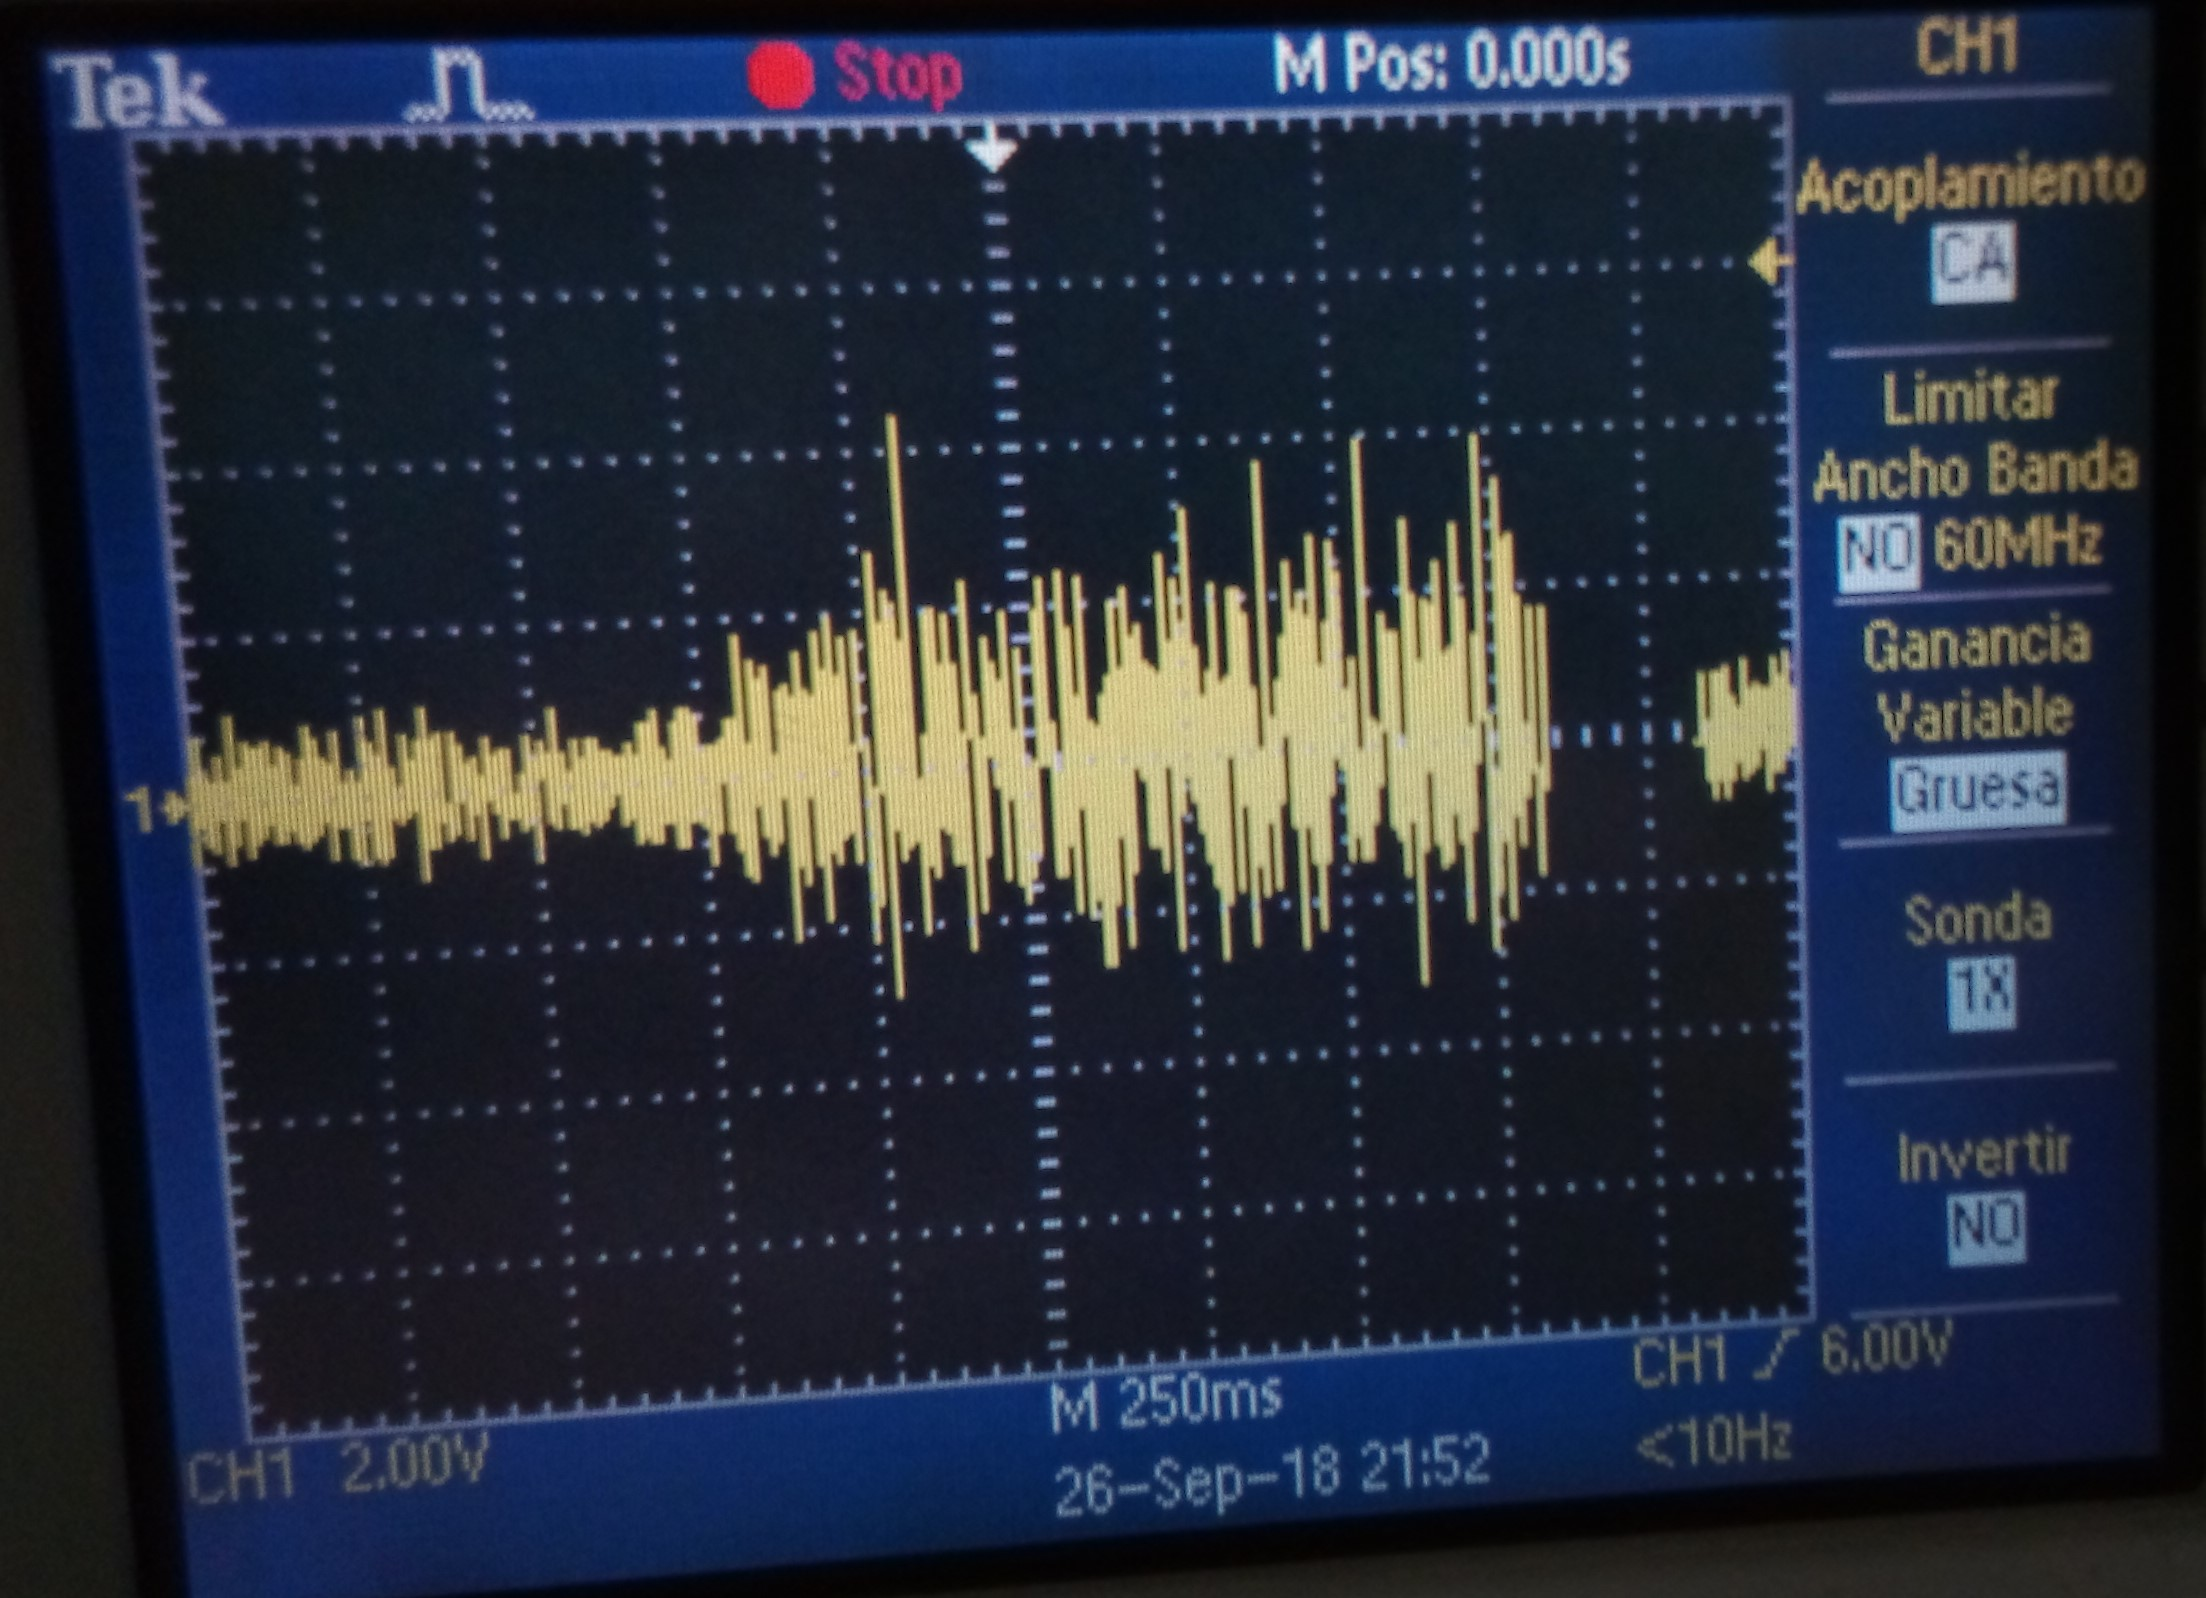
\includegraphics[width=0.75\textwidth]{Practica3/images/filtrada8.jpg}
            \end{figure}
            
            
            
	\subsubsection{Comparación con respecto al Circuito 1}
	
	Como se observa, la segunda salida, con respecto a la primera salida, cuando no se ejerce fuerza, la señal sale estable, con el ruido mínimo, aunque no eliminado por completo. Esto representa un ligero problema pues también se amplifica en la salida de la señal que deseamos obtener. 
	
	Además, también se nota que ahora la señal sale con una amplitud máxima de 10 Vpp, que es lo esperado para proceder a la siguiente etapa.
	
	Por último, añadimos un capacitor de $0.1 \mu F$ a la señal de salida antes de medirla, junto a 2 resistencias de $47 k \Omega$ que van a tierra. Este decisión es para manejar el error de medición que se amplifica y evitar inconvenientes al integrar el vúmetro al circuito.
	
	
	\subsection{PE 3 - Circuito 3: Vúmetro}
	\subsubsection{Esquema}
	\begin{figure}[h!]
                \centering
                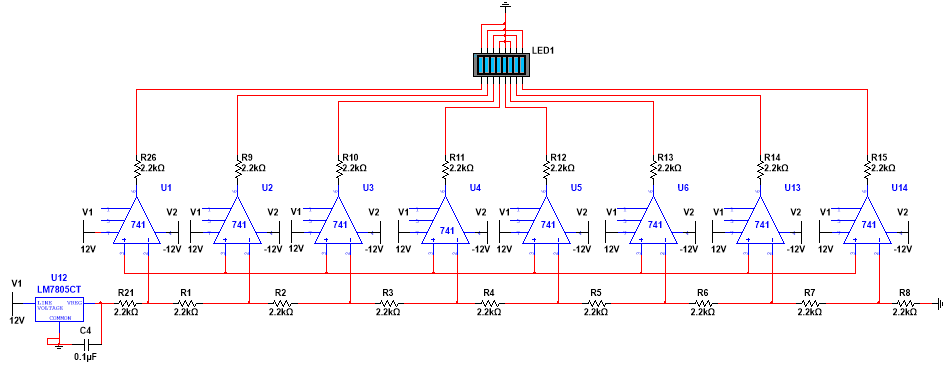
\includegraphics[width=0.95\textwidth]{Practica3/images/cvumetro.PNG}
    \end{figure} 
    \newpage
	\subsubsection{Circuito cableado}
		\begin{figure}[h!]
                \centering
                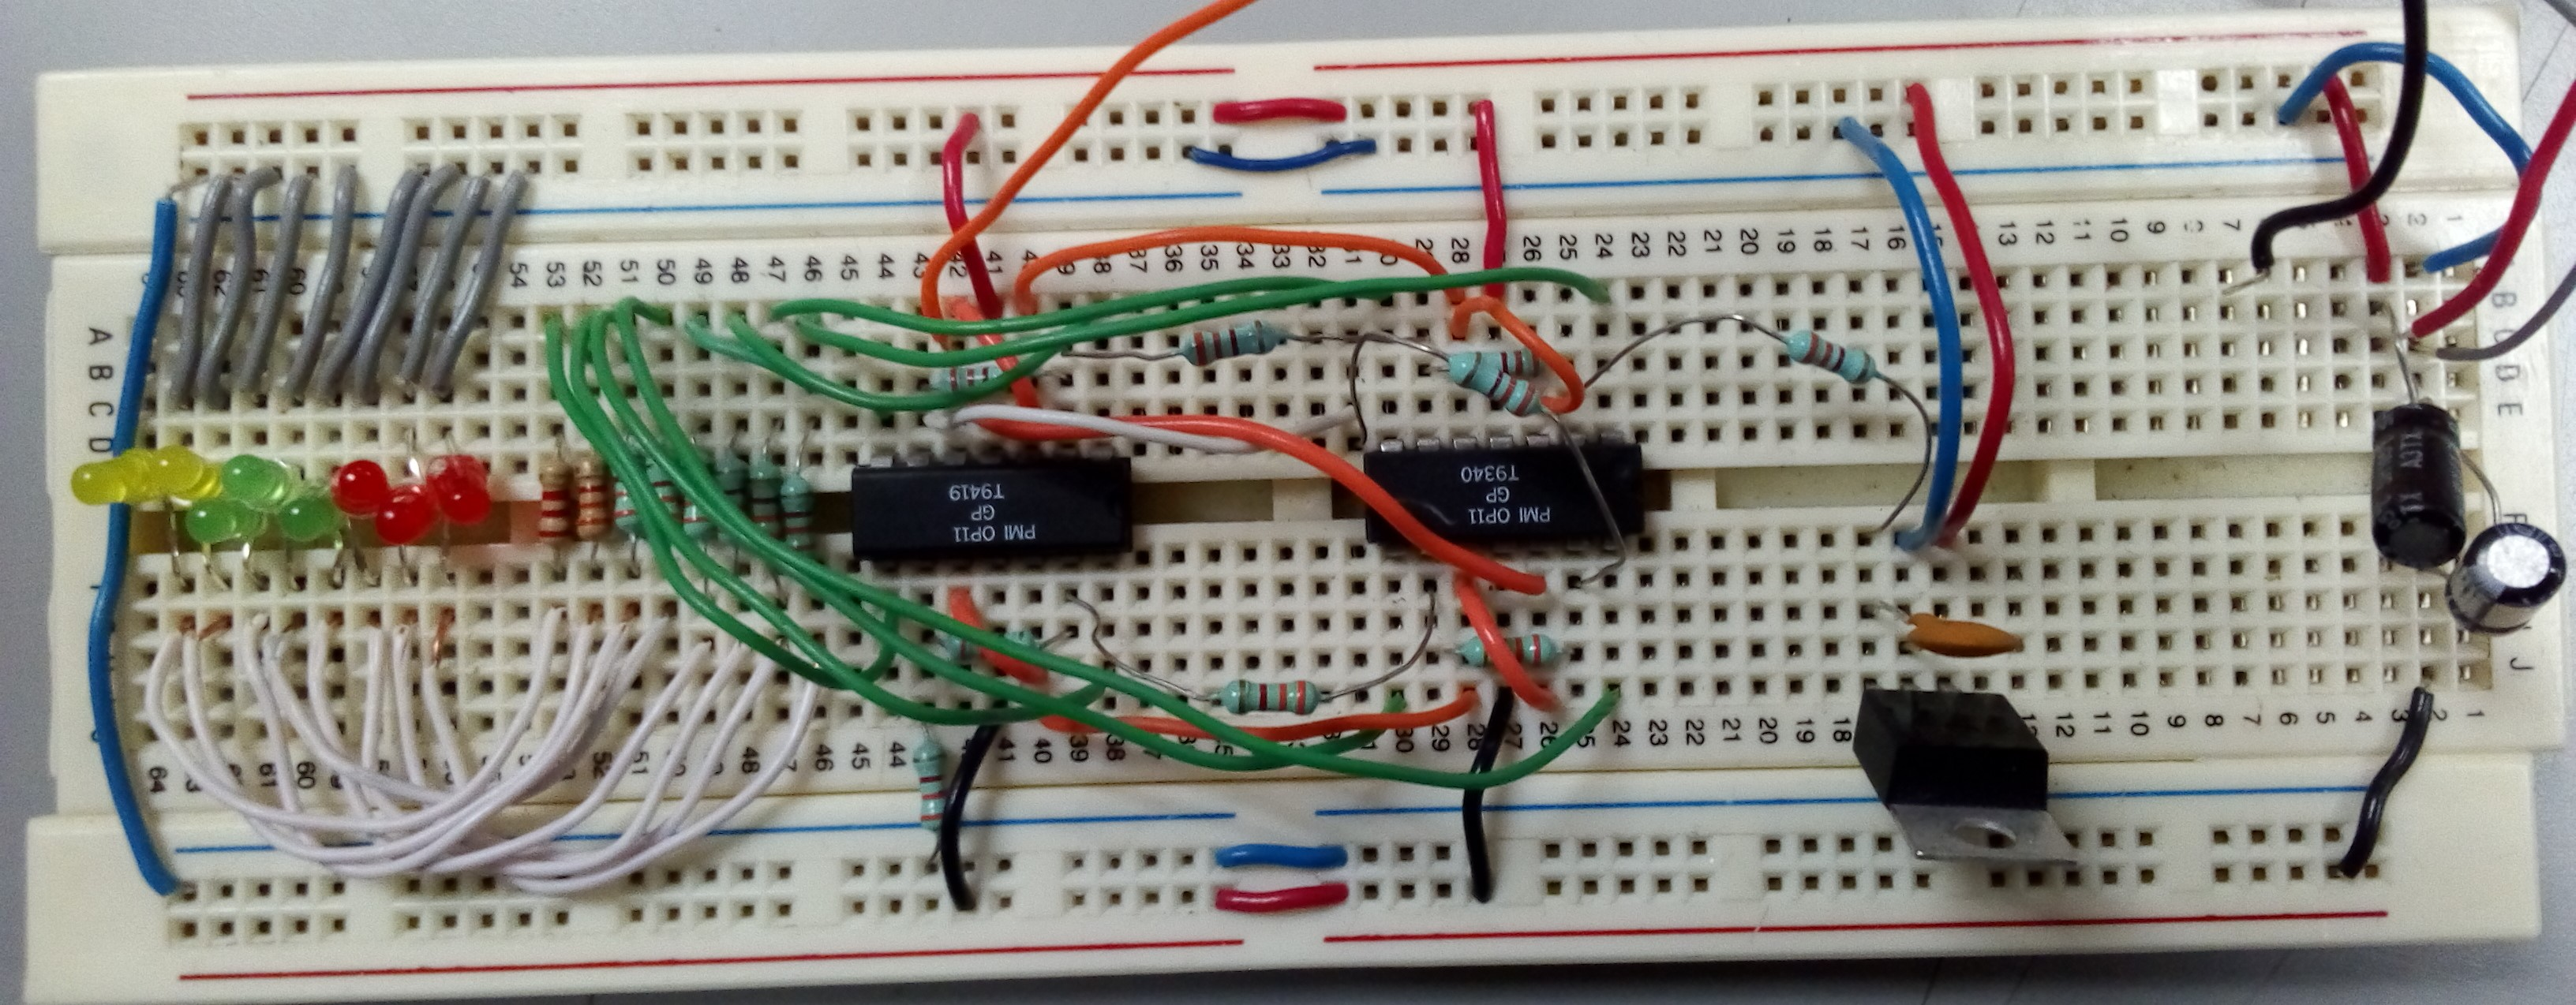
\includegraphics[width=\textwidth, angle=180]{Practica3/images/cvumetro4.jpg}
    \end{figure} 
    
    
	\subsubsection{Funcionamiento del vúmetro}
	La señal de salida amplificada obtenida en la fase anterior se conecta en serie a las entradas no inversoras de los 8 amplificadores operacionales. Además, el voltaje de la fuente de alimentación pasa por un regulador de voltaje 7805 para estabilizarlo a 5V constantes, que irán directos a cada resistor de las entradas inversoras de los 8 amplificadores.
	        
	De tal forma que se tiene un divisor de voltaje para reducir la amplitud de la señal de entrada. La señal varia de acuerdo a la tensión de músculo que se ejerce, detectada por los electrodos, y hace que el arreglo de 8 LEDs enciendan de acuerdo al nivel de voltaje de la señal.
	        
	En este caso, mientras más tensa sea la señal del músculo detectada por los electrodos, significa que se esta apretando con fuerza, enviando una señal con la amplitud máxima que viajara hasta el vúmetro, provocando que los LEDs que enciendan emulando una escala del verde (músculo relajado) al rojo (músculo tenso y contraído, aplicando fuerza sobre él).
	        
	Los siguientes datos se justifican en la sección de anexo: 
	        
	\textbf{Rango de medición (voltaje):} $0.55 V$ a $4.44 V$
	        
	\textbf{Resolución (voltaje):} $0.55 V$
	
	\newpage
	\subsection{Circuito Completo}
	\subsubsection{Esquema}
	\begin{figure}[h!]
                \centering
                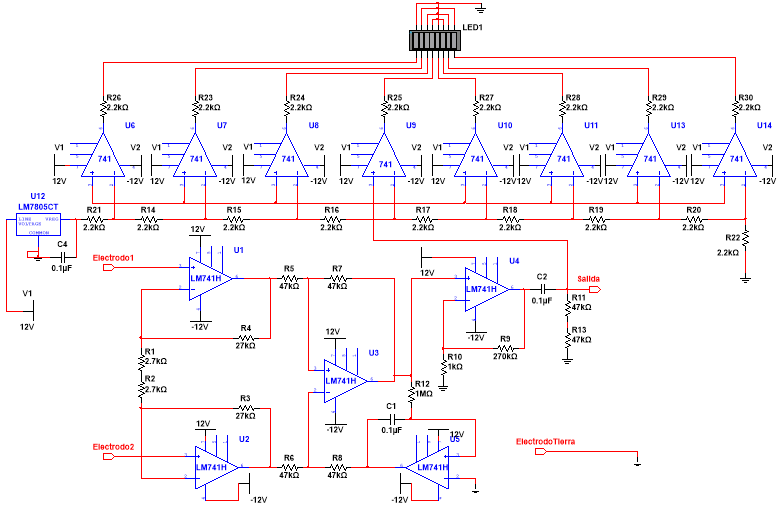
\includegraphics[width=1.05\textwidth]{Practica3/images/ccompleto.PNG}
    \end{figure} 
    
    \subsubsection{Funcionamiento general}
    Los electrodos se conectan alrededor de un brazo,  de esta forma que al hacer contracción generará señales eléctricas conocidas como electromiográficas, dicha señal es procesada por el amplificador de instrumentación el cual genera la diferencia de las señales de ambos electrodos, eliminando el ruido existente.
    
    Sin embargo, en ocasiones ocurre que dicho ruido no es eliminado del todo, tal como lo fue en nuestro caso, por eso es necesario agregar un filtro que limpiara la señal del amplificador de instrumentación.
    
    Cuando ya tenemos una señal limpia, usamos el vúmetro que nos ayuda a visualizar como se esta comportando la señal recibida. Cuando el sujeto de prueba hace contracción se muestra en el osciloscopio el cambio en la señal y en el vumetro se prenden los leds de manera gradual.

    
    \newpage
	\subsubsection{Circuito cableado}
		\begin{figure}[h!]
                \centering
                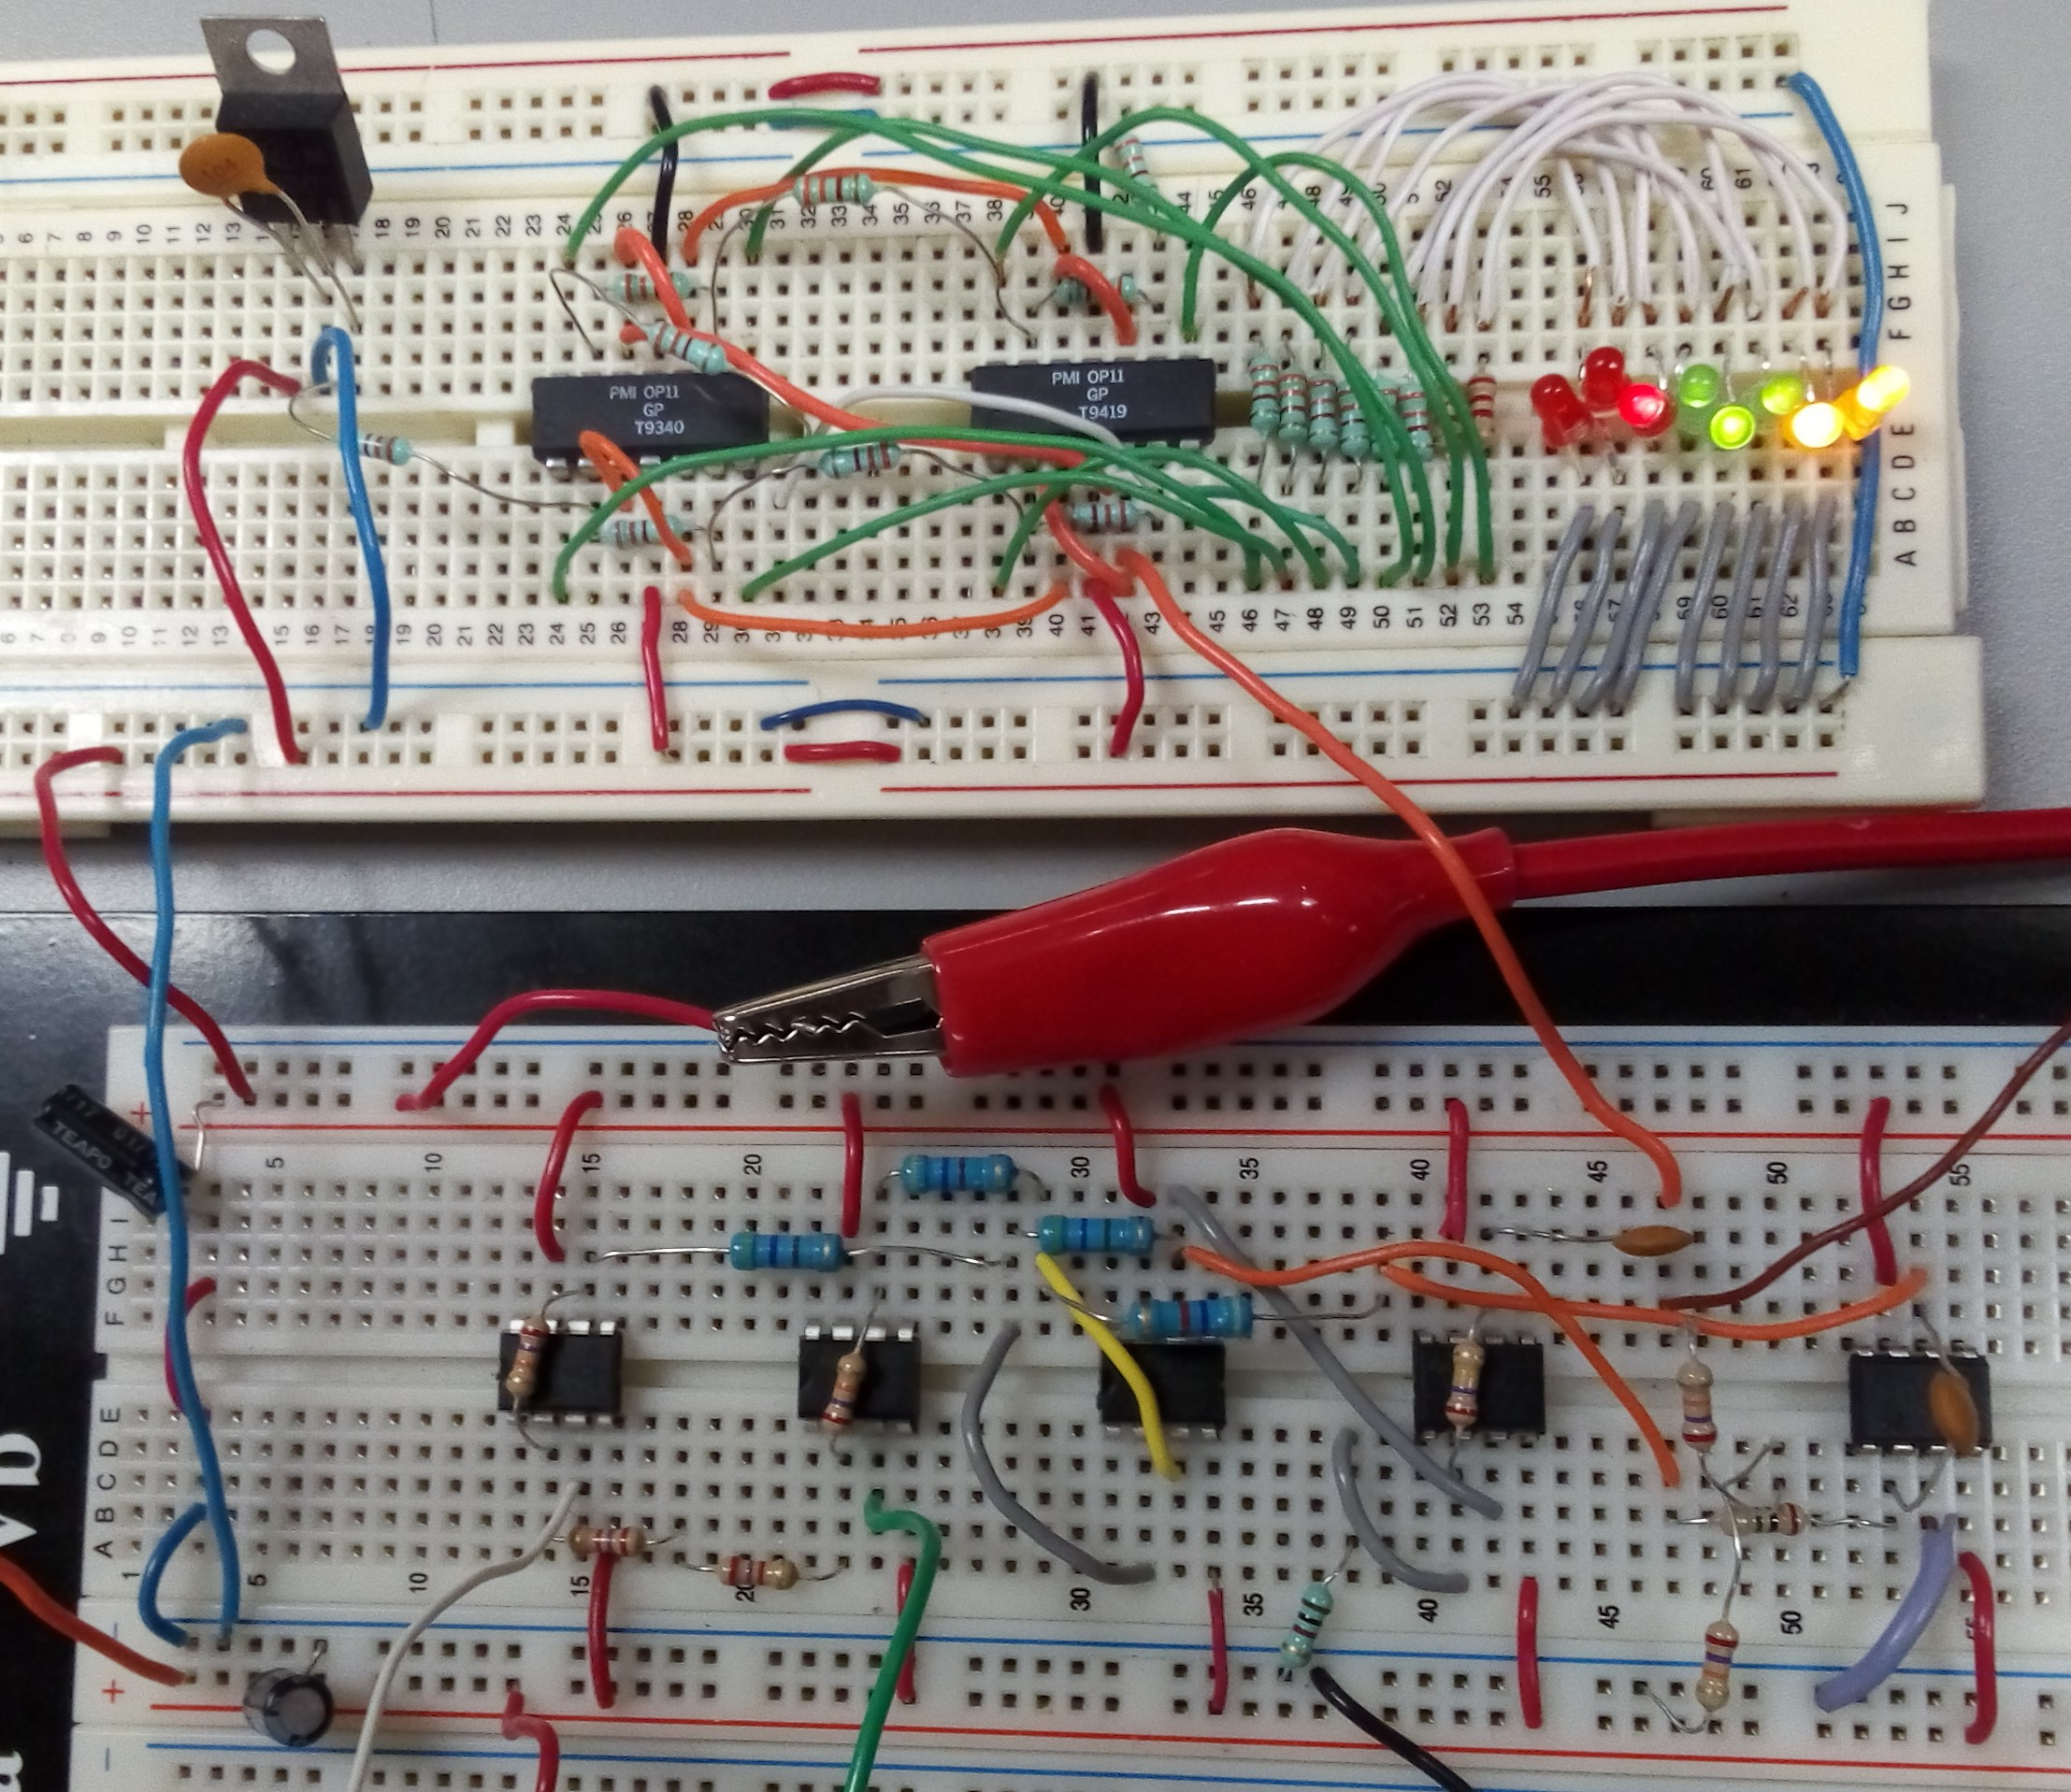
\includegraphics[width=0.73\textwidth]{Practica3/images/completo.jpg}
    \end{figure} 
    
    \begin{figure}[h!]
                \centering
                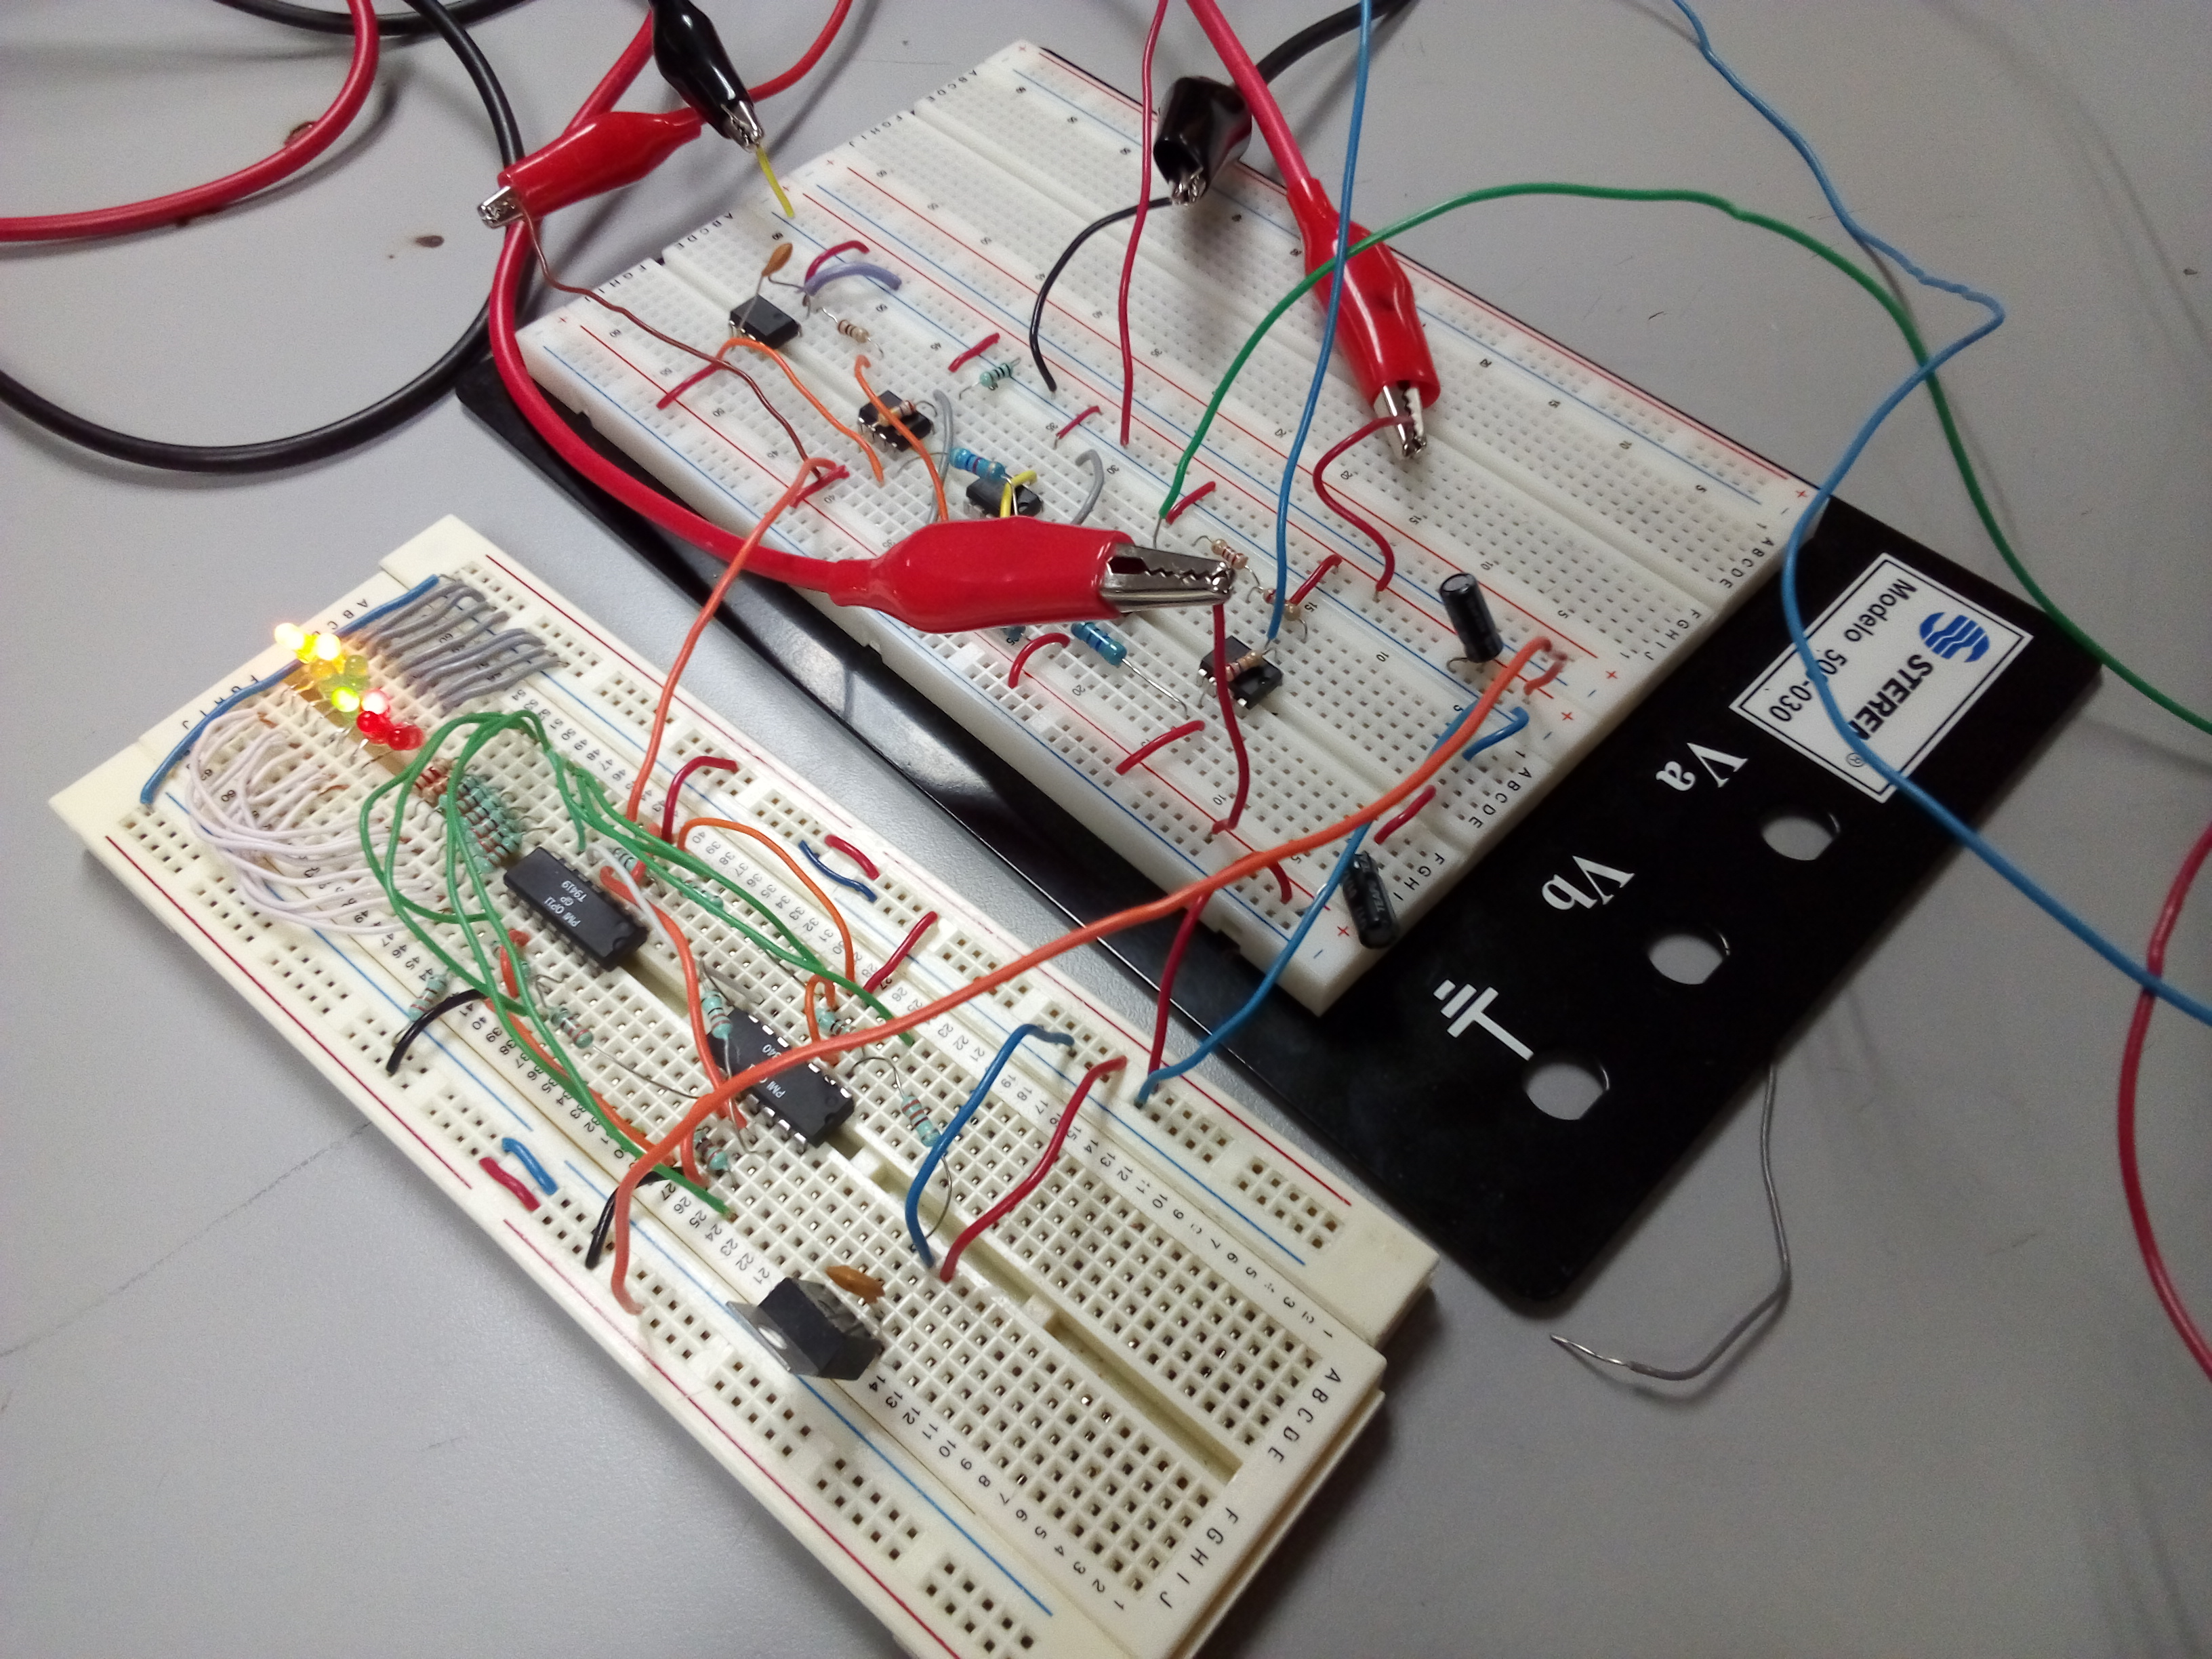
\includegraphics[width=0.73\textwidth]{Practica3/images/completo8.jpg}
    \end{figure} 
    
        \newpage
    \textbf{Músculo del brazo relajado:}
    \begin{figure}[h!]
                \centering
                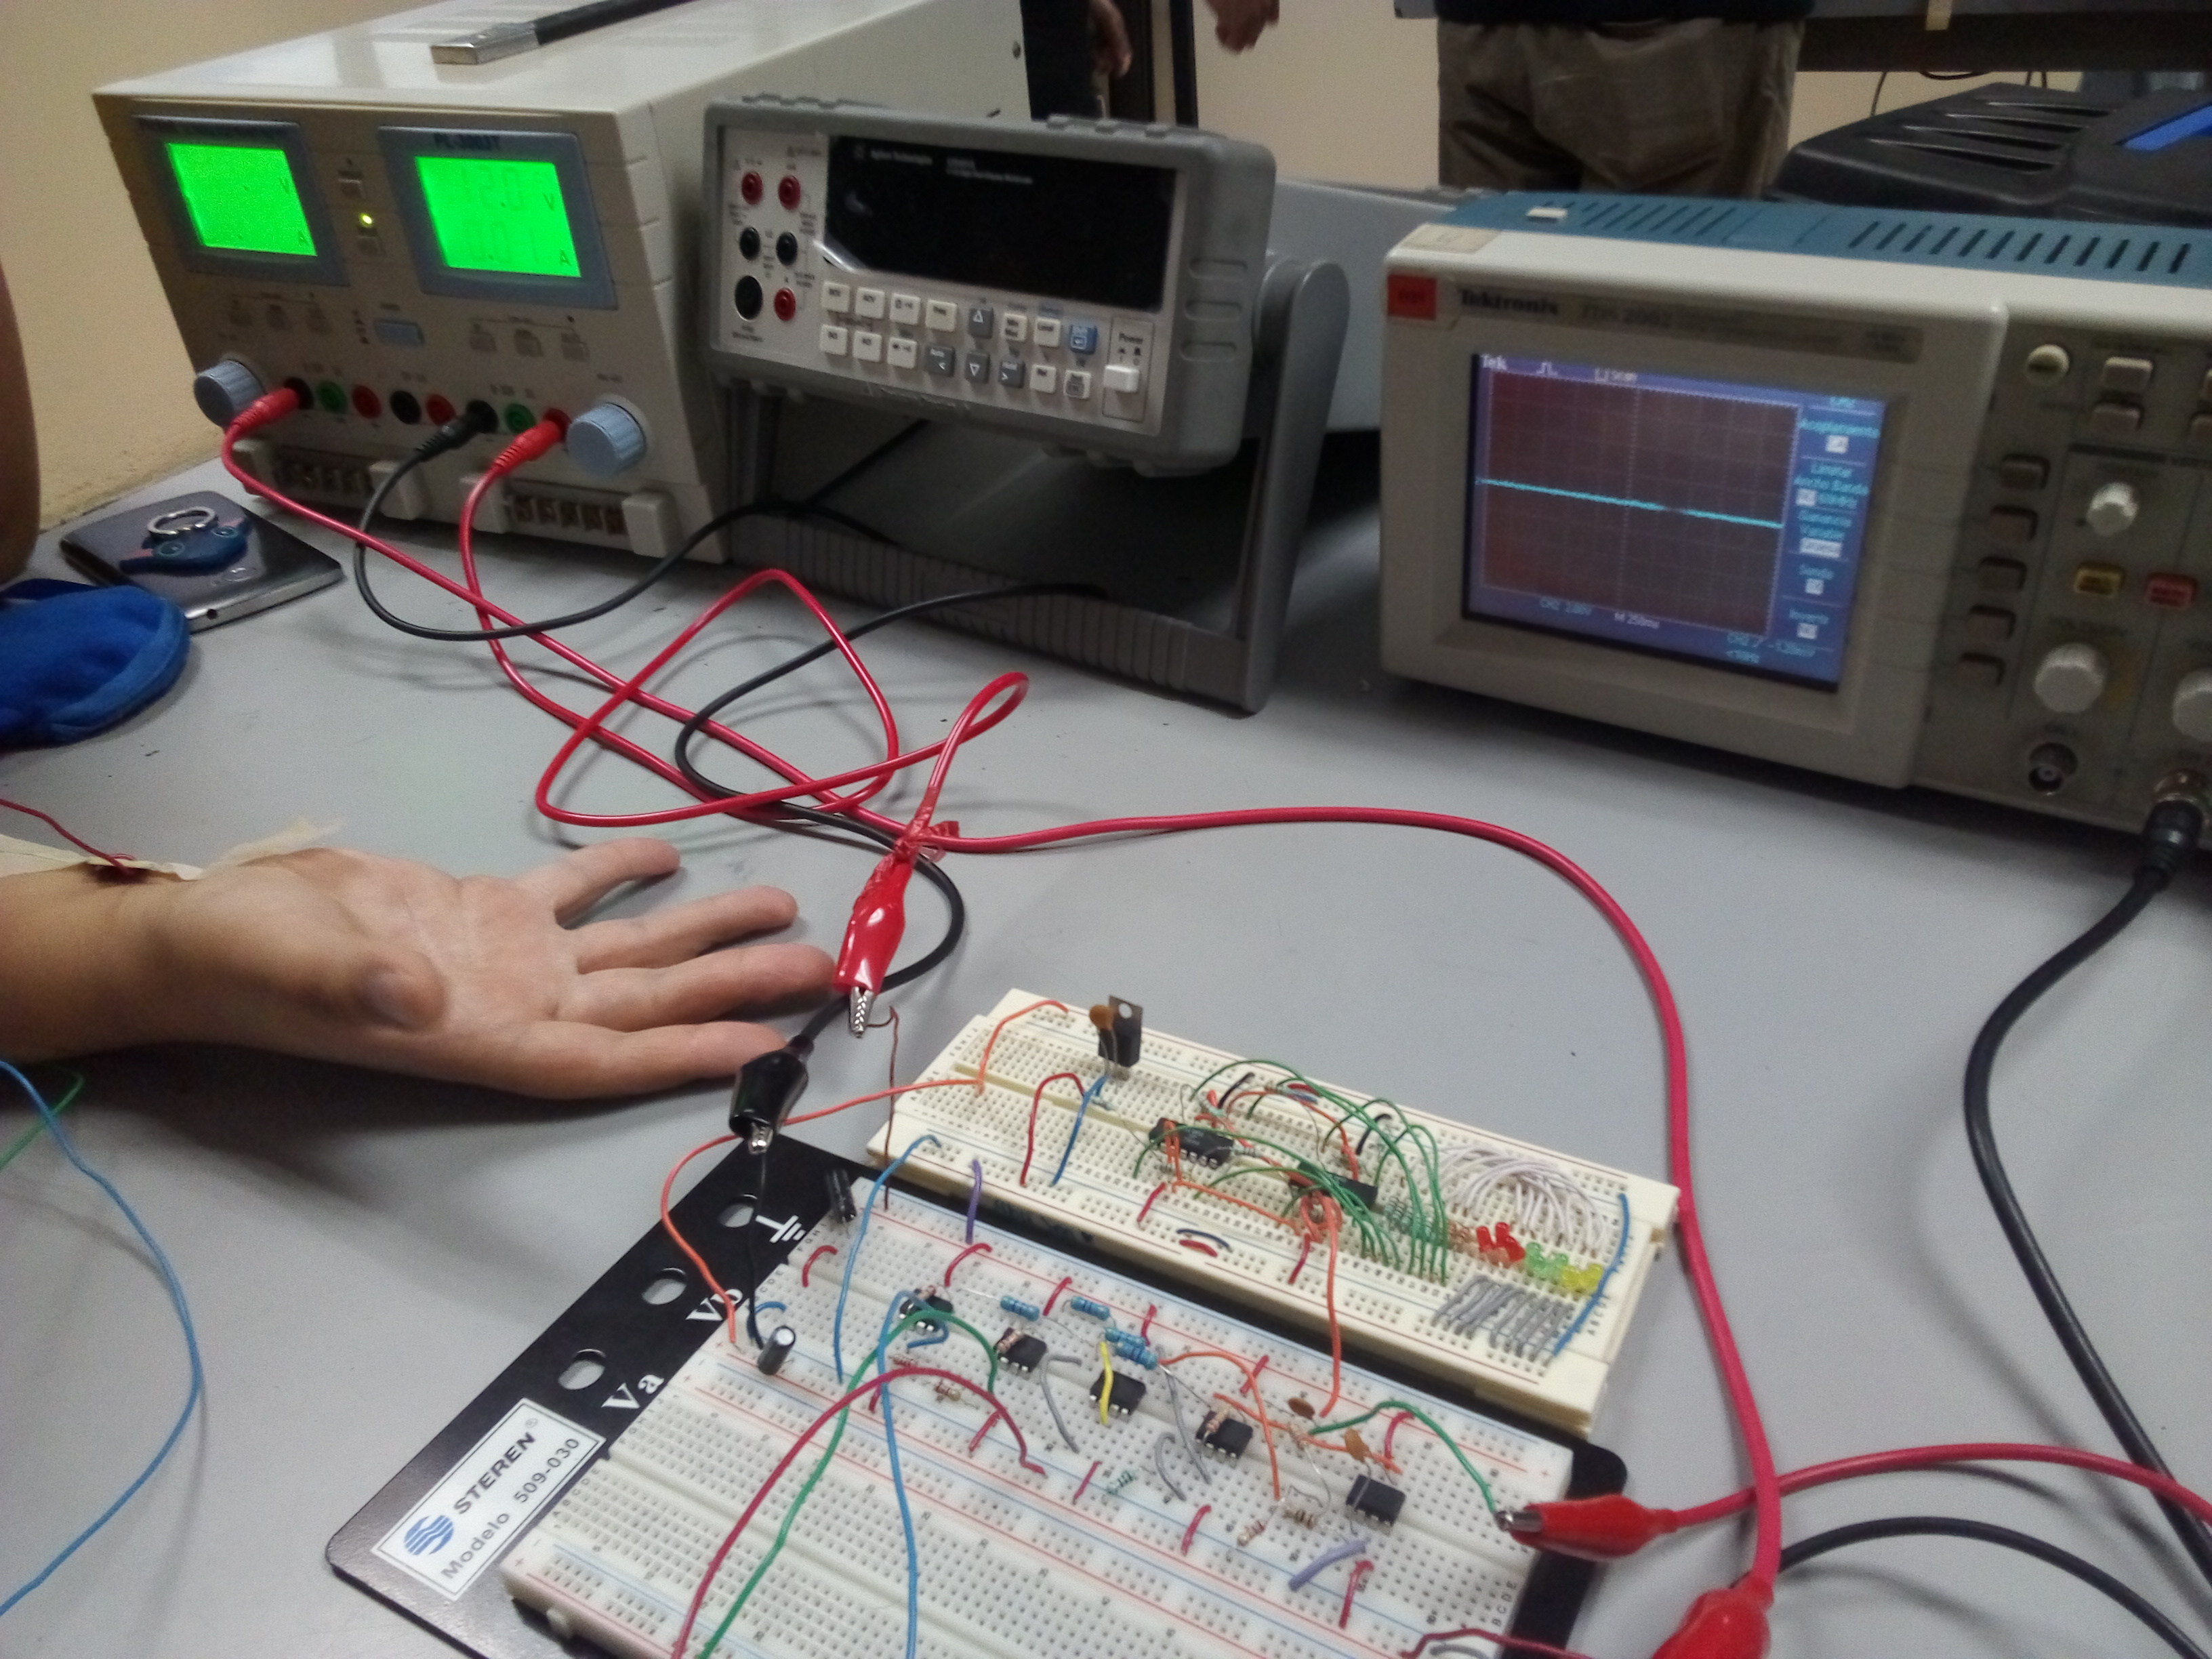
\includegraphics[width=0.8\textwidth]{Practica3/images/relajado.jpg}
    \end{figure} 
    
    \begin{figure}[h!]
                \centering
                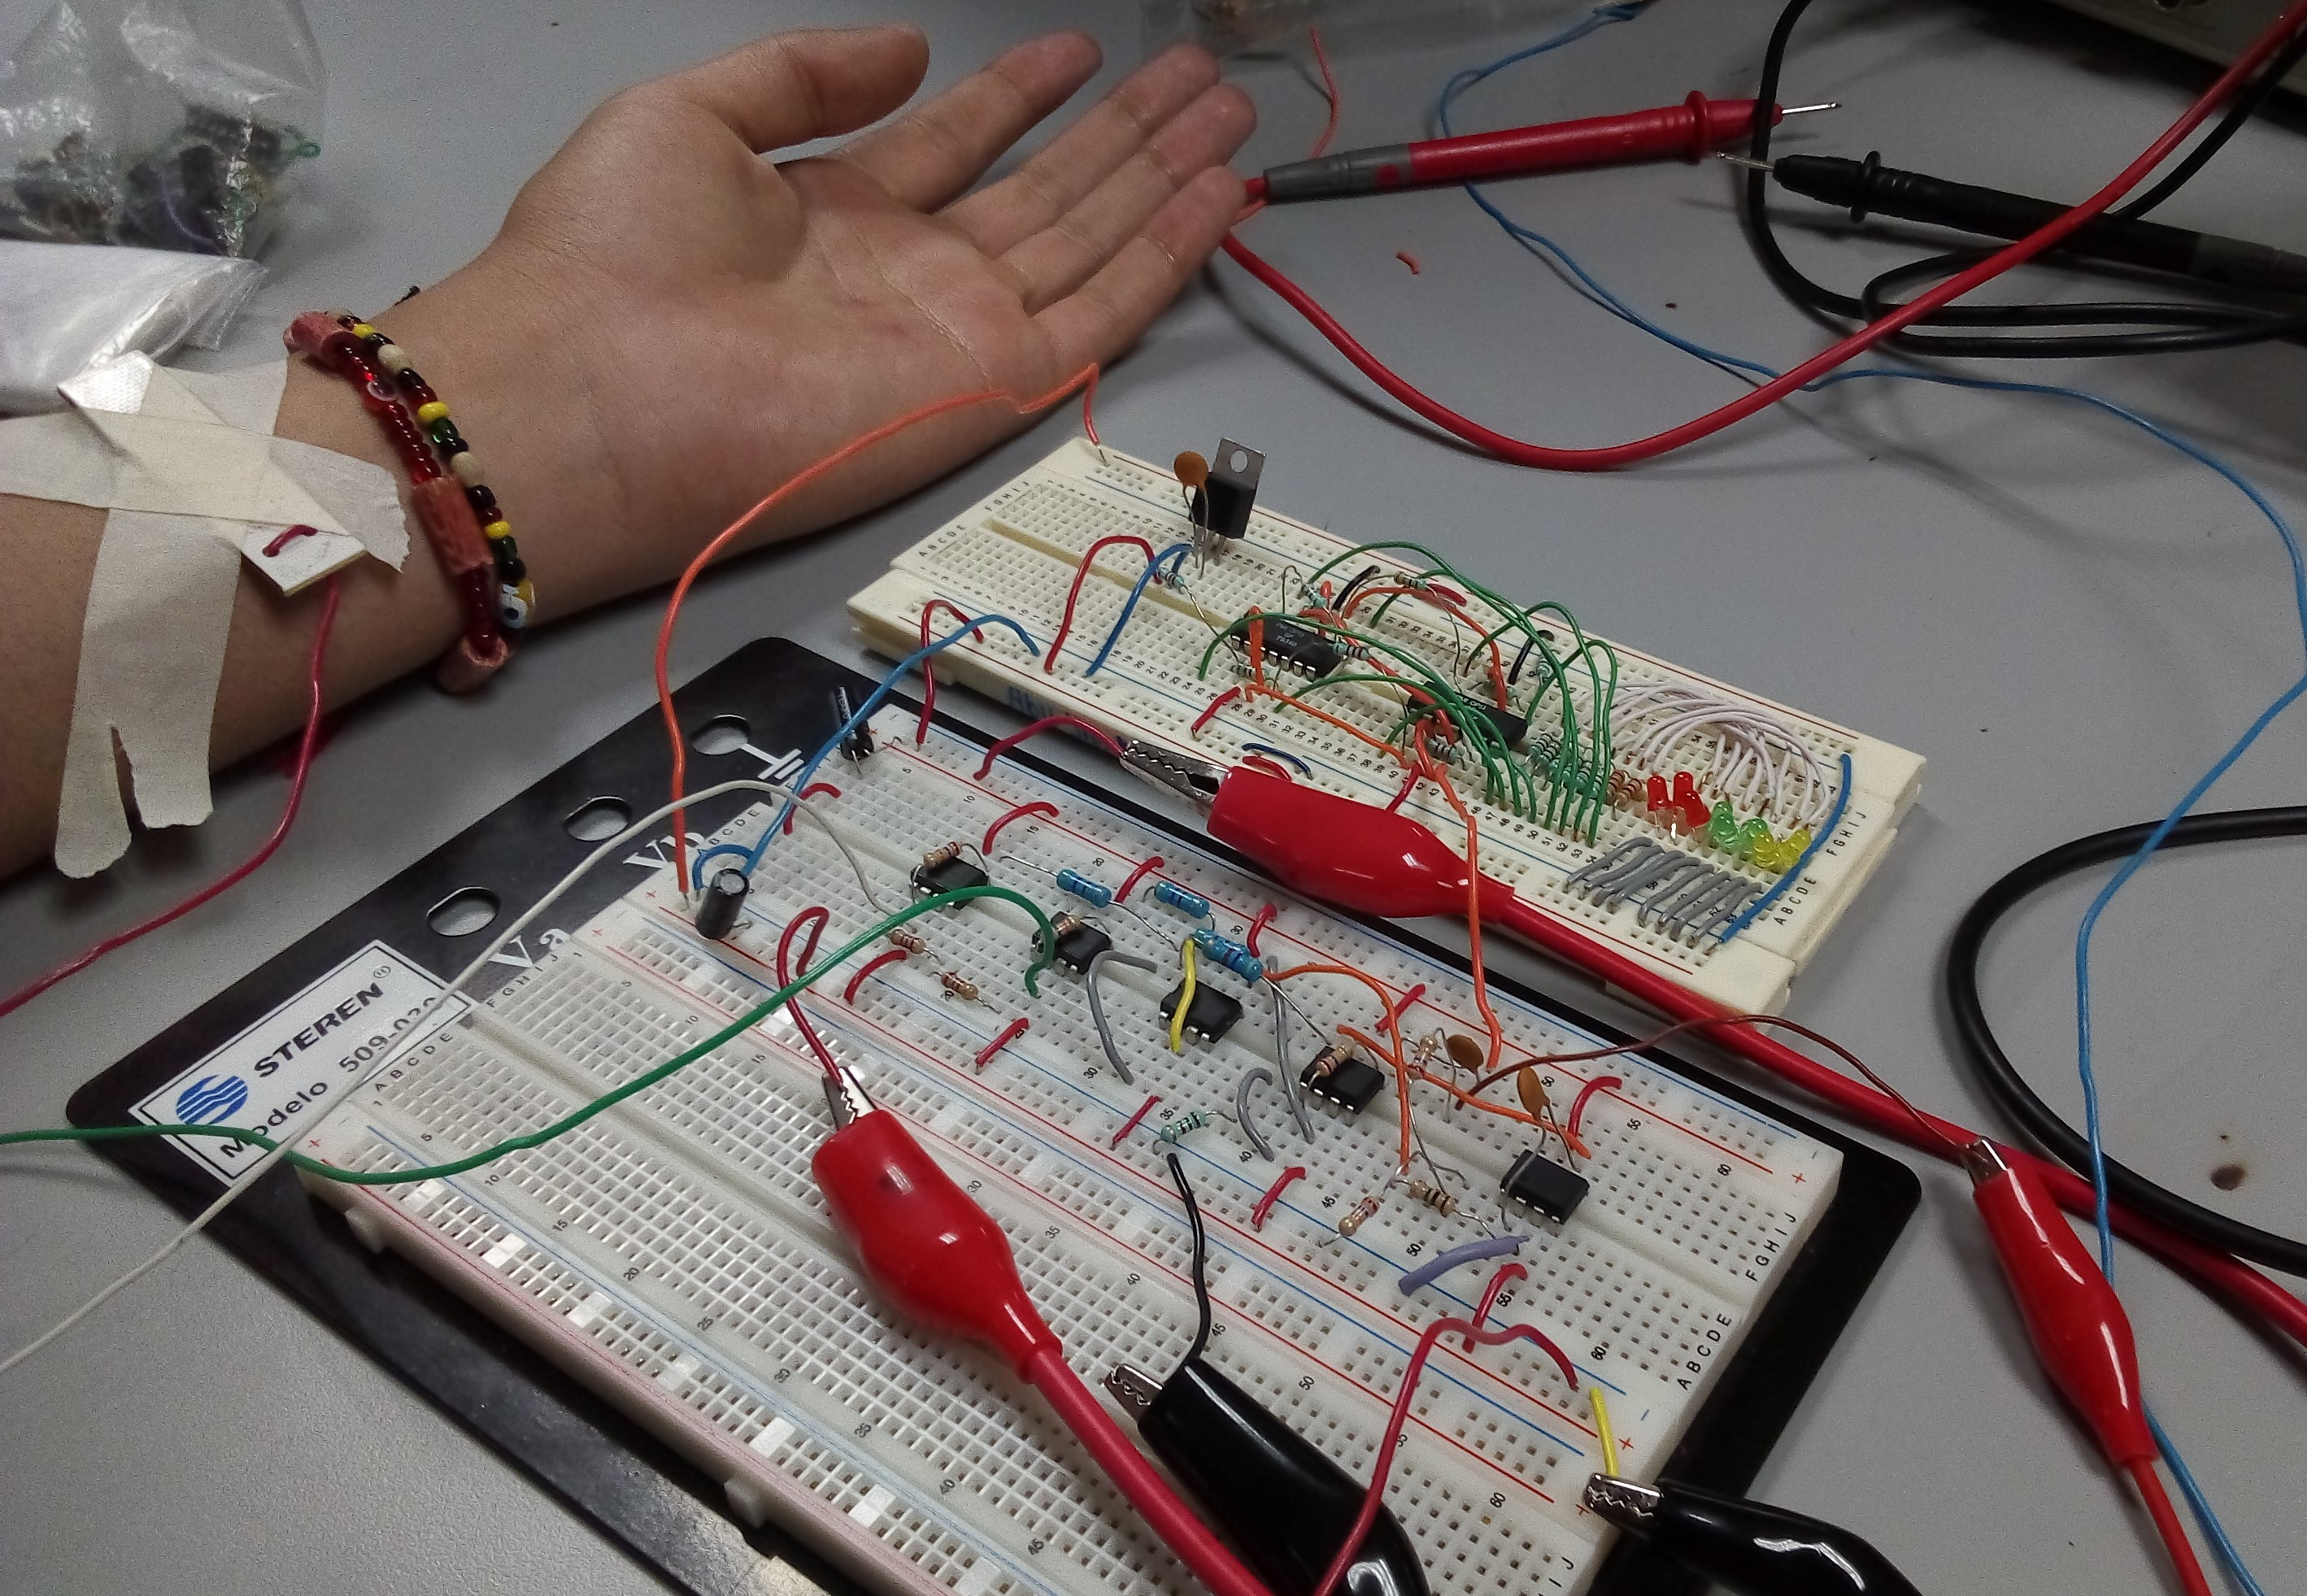
\includegraphics[width=0.8\textwidth]{Practica3/images/relajado3.jpg}
    \end{figure} 
    \newpage
        \textbf{Músculo del brazo tenso:}
    \begin{figure}[h!]
                \centering
                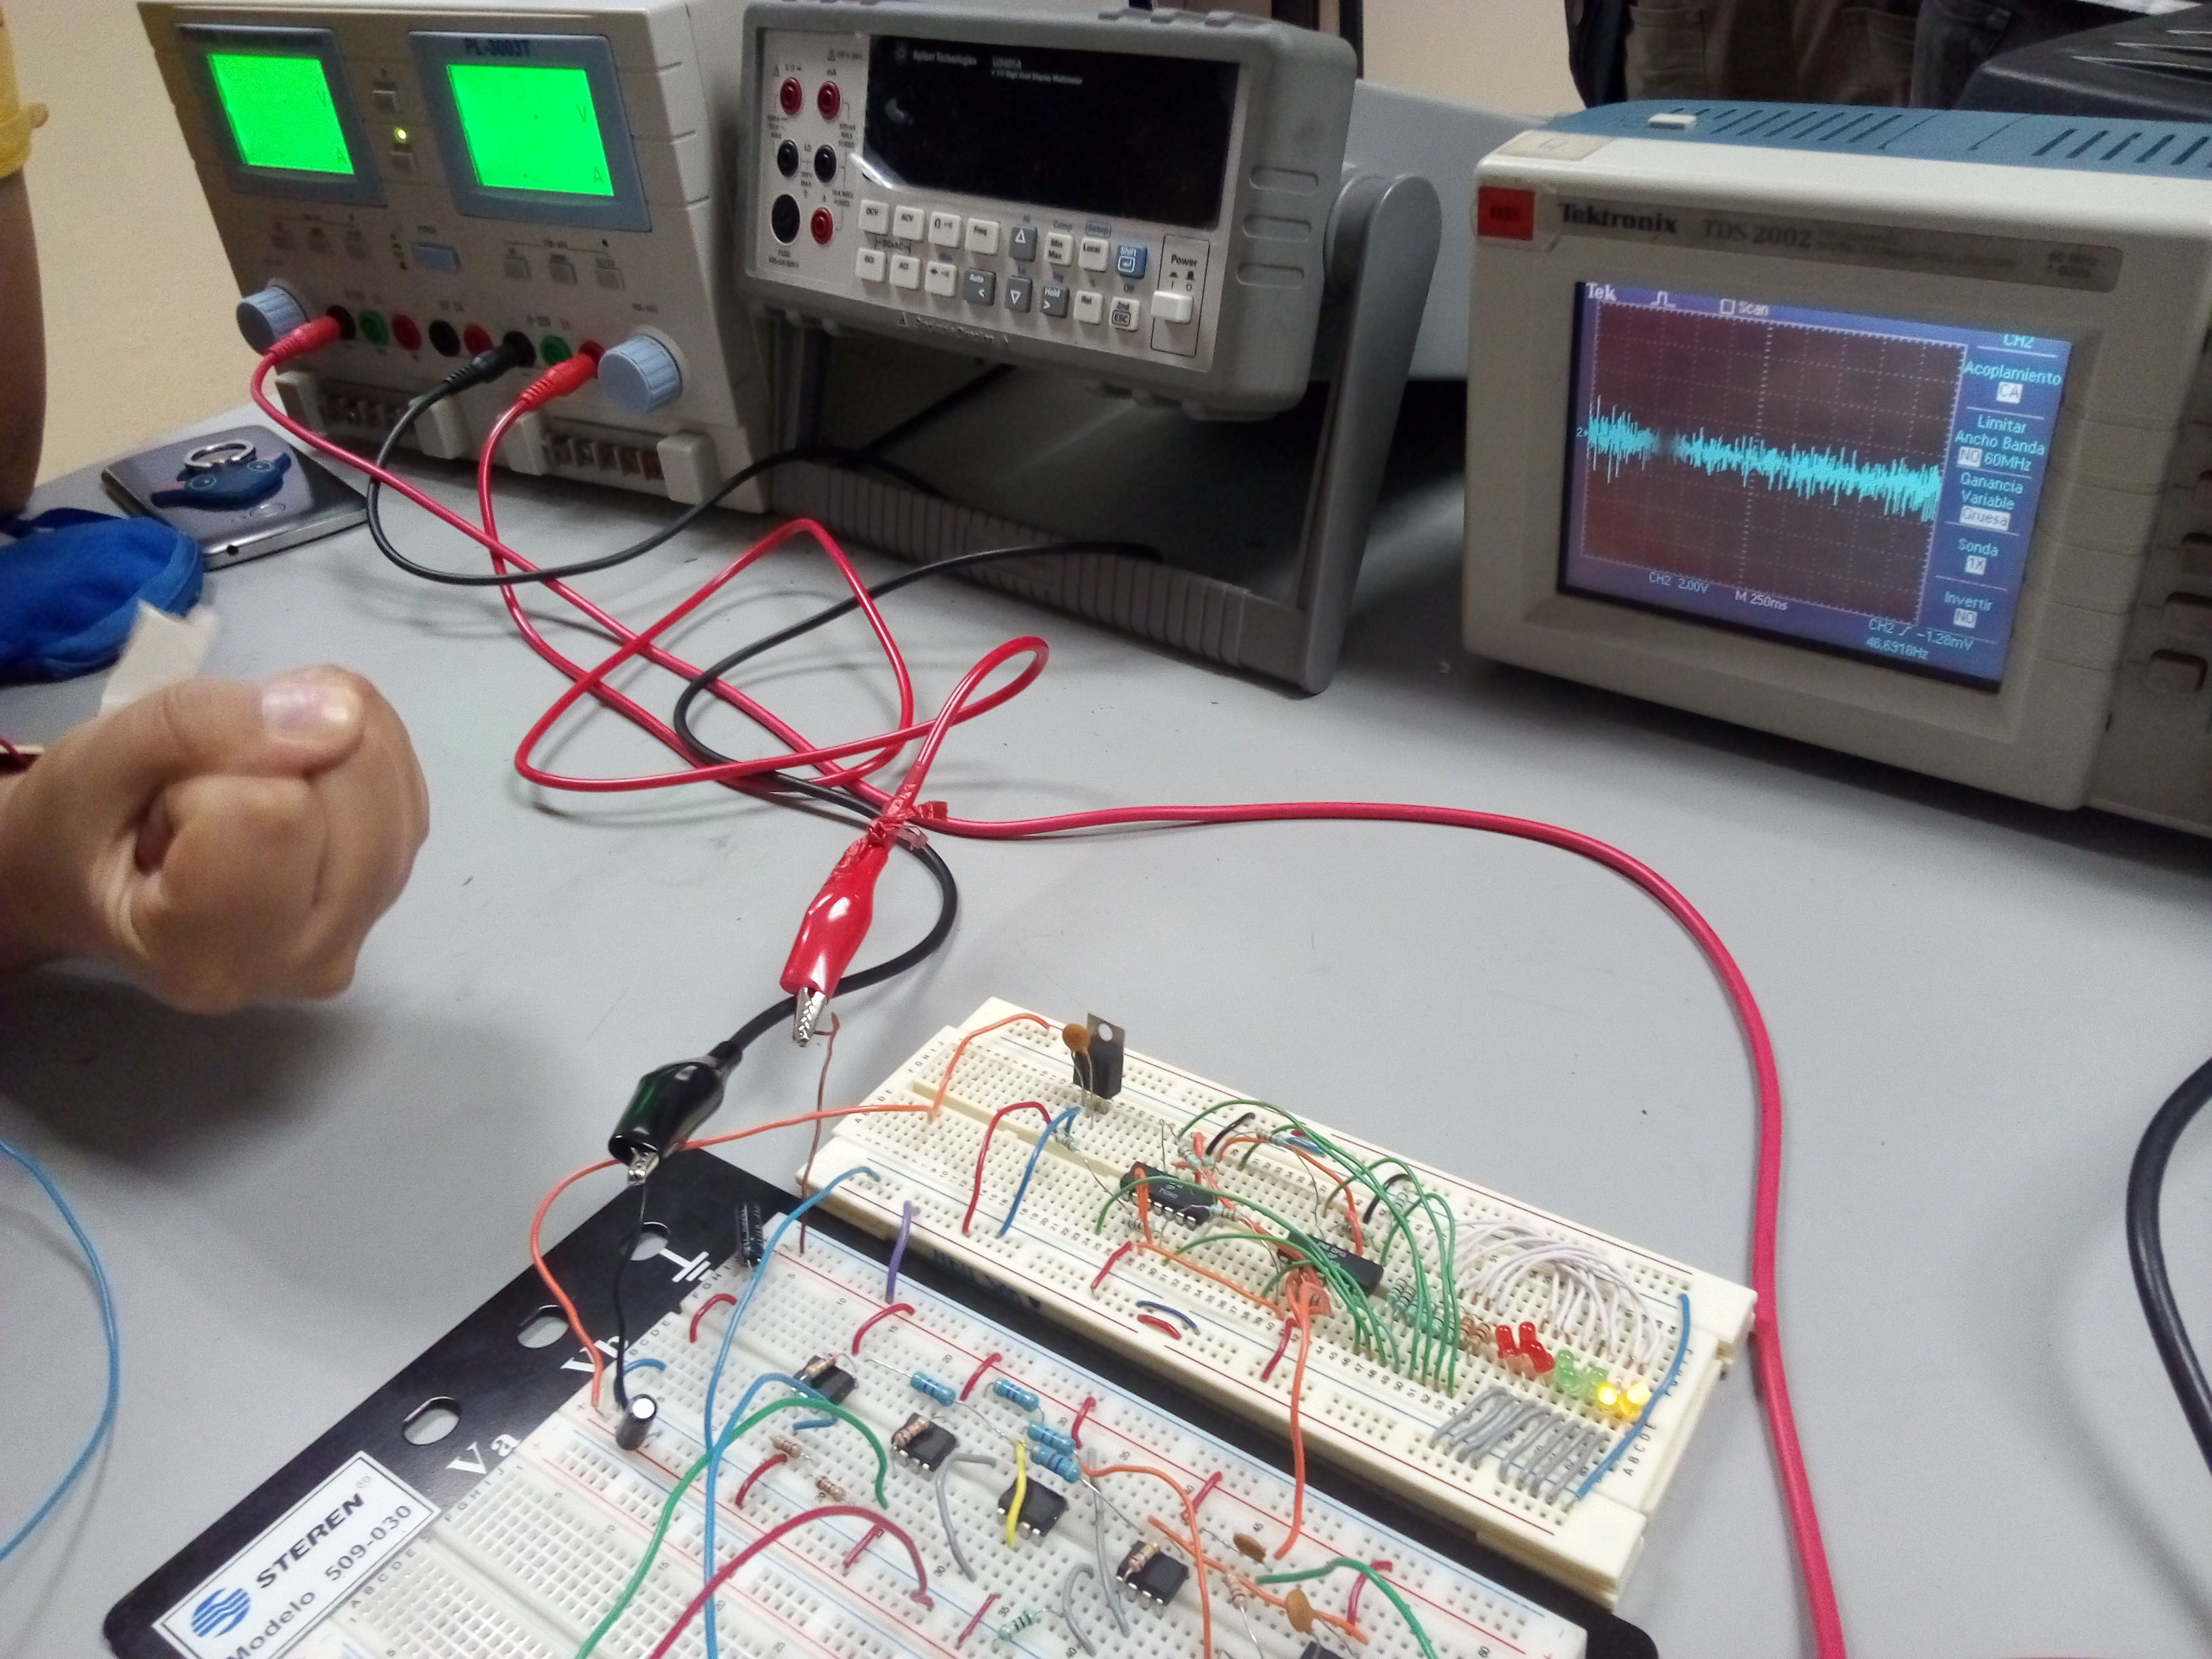
\includegraphics[width=0.8\textwidth]{Practica3/images/tenso.jpg}
    \end{figure} 
    
    \begin{figure}[h!]
                \centering
                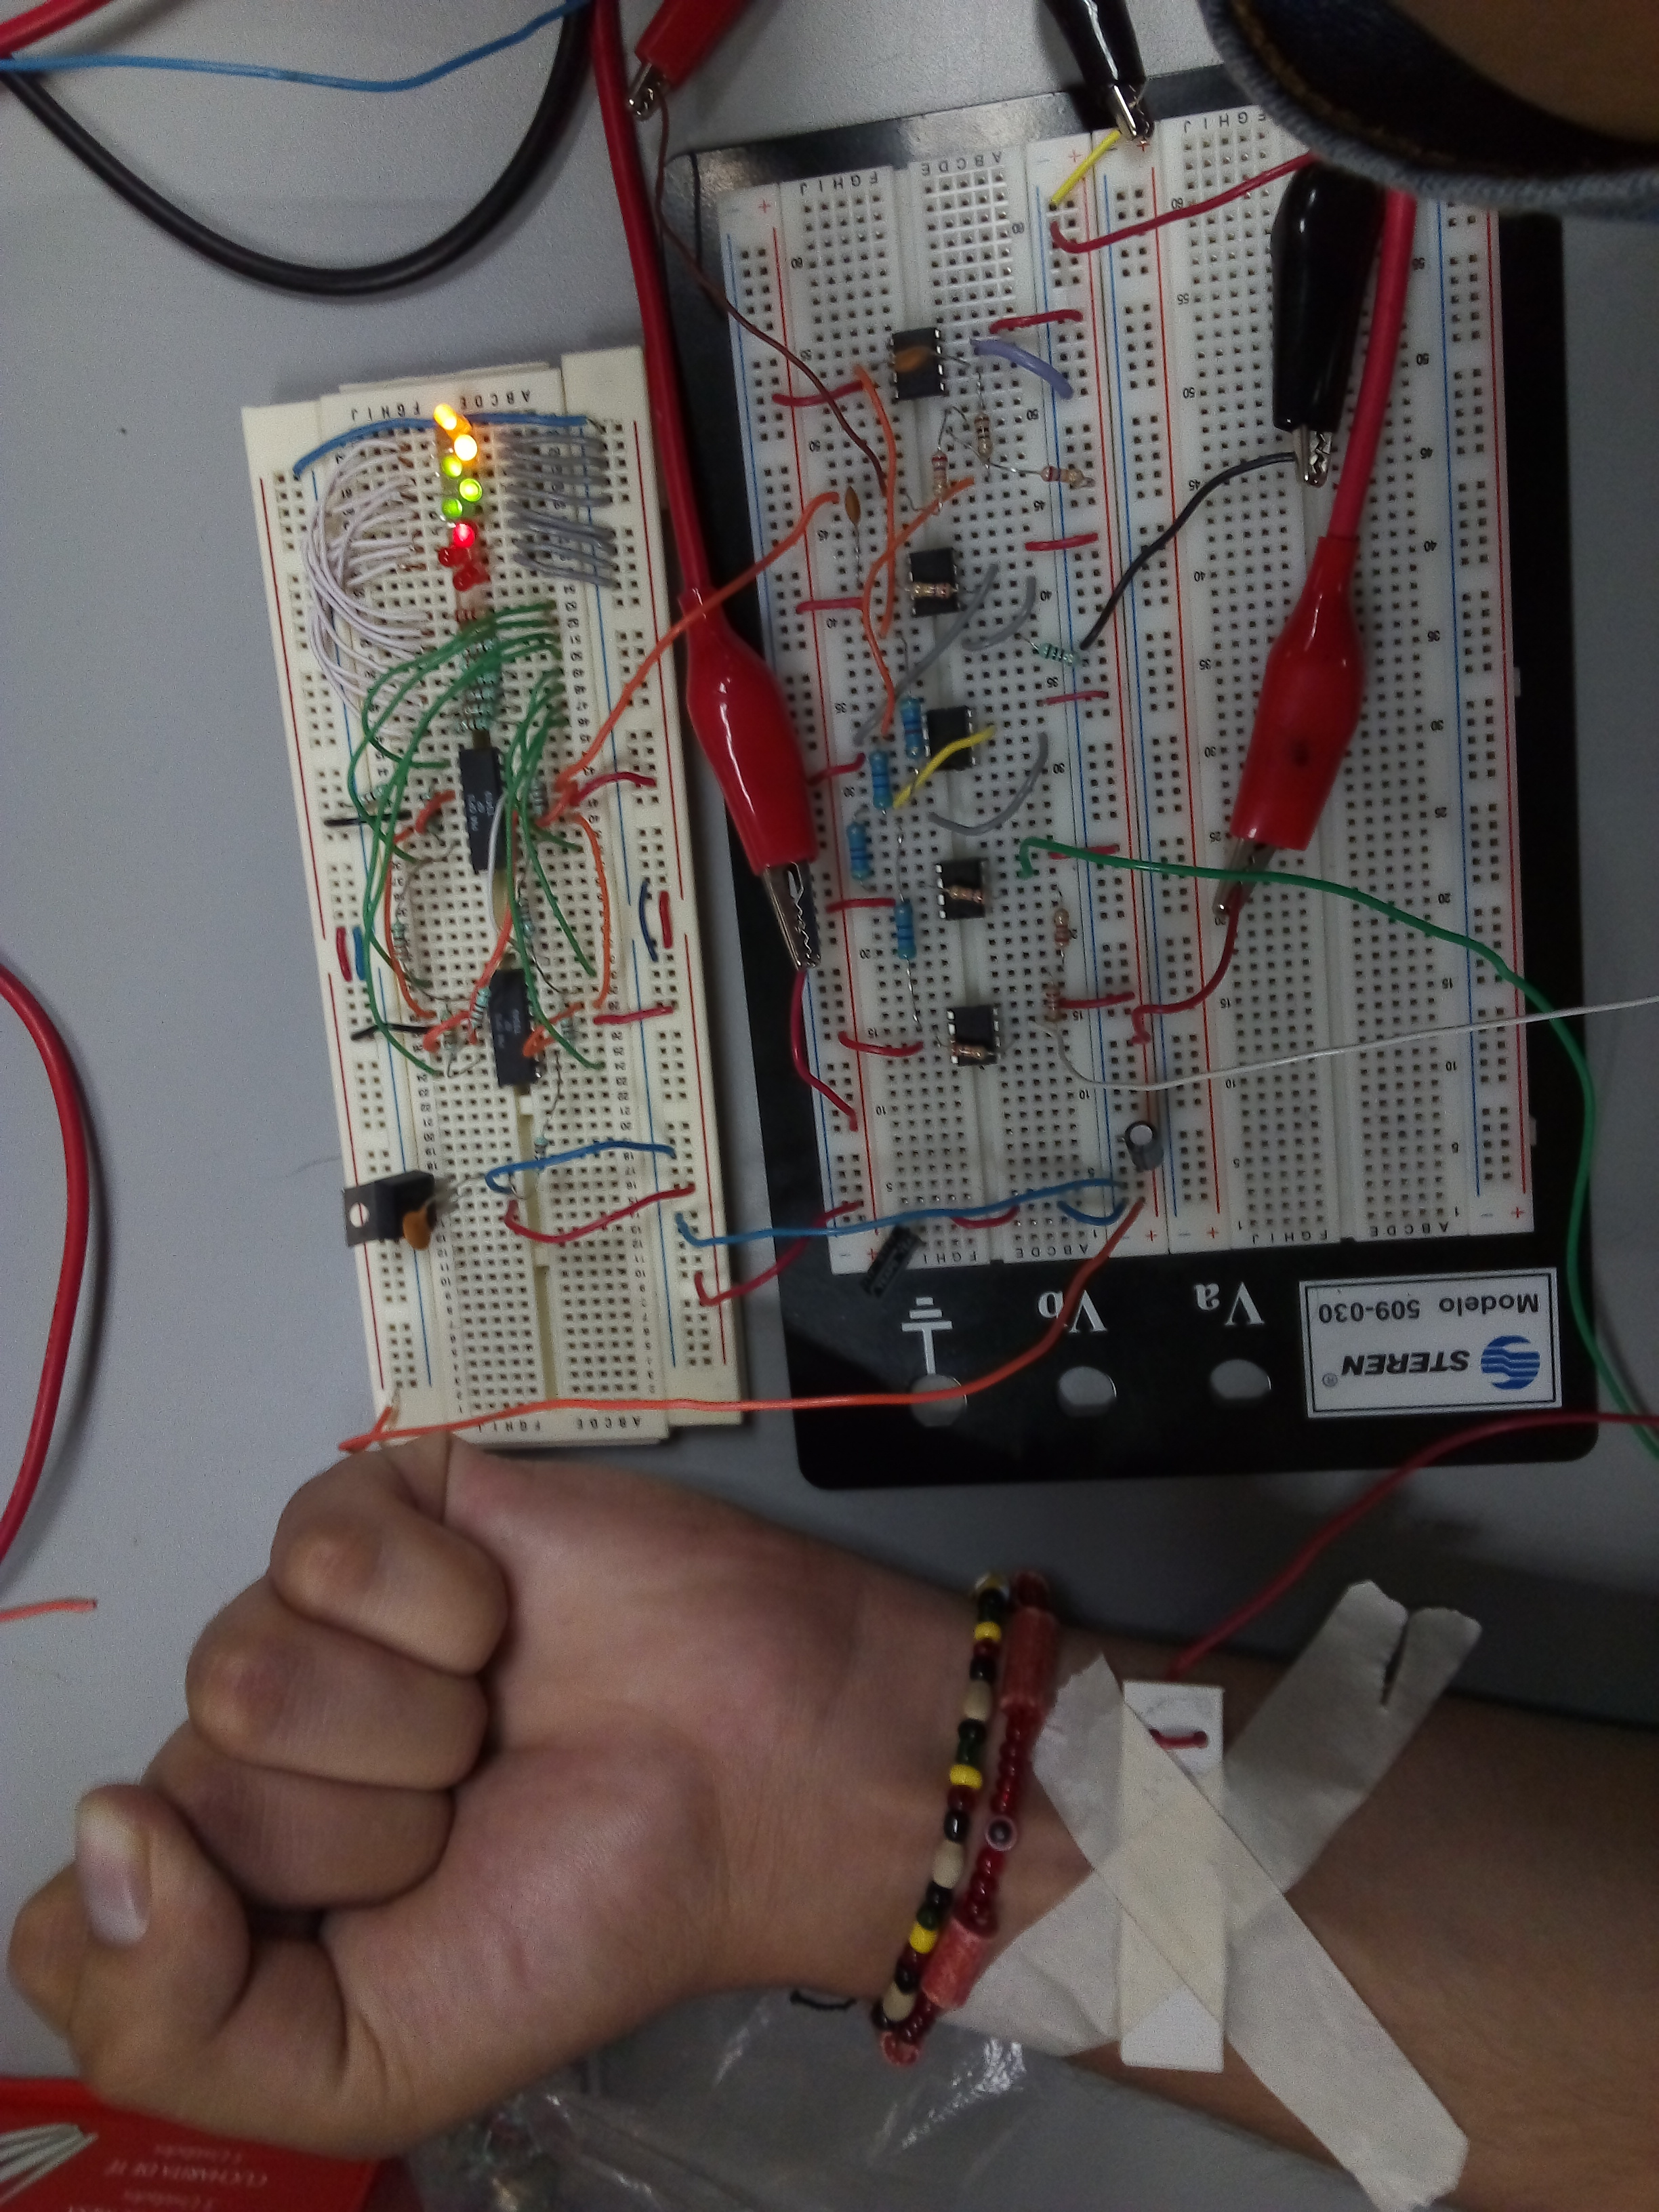
\includegraphics[width=0.6\textwidth, angle=-90]{Practica3/images/tenso2.jpg}
    \end{figure} 
	

	
	% /////////////////////////////////////////////////////////////////////
	%							OBSERVACIONES
	% ////////////////////////////////////////////////////////////////////
	\newpage
	\section{Observaciones}
	
	\begin{itemize}
            \item[\checkmark] Es importante que los electrodos tengan como mínimo 50 cm de longitud, y dimensiones de entre 5x3 cm y 8x5 cm.
            \item[\checkmark] Los electrodos deben ser limpiados con ayuda de una goma azul antes de colocarlos en la superficie de la piel en el músculo del brazo.
            \item[\checkmark] El acoplamiento del osciloscopio al medir las señales mioelectricas del brazo debe estar en Corriente Alterna
            \item[\checkmark] Sin embargo, al momento de medir las señales con el vúmetro, se tomará en cuenta el acoplamiento en Corriente Continua.
            \item[\checkmark] Respecto al acoplamiento del punto anterior, observando el funcionamiento del vúmetro, notamos que la tira de LEDs siempre permanecía encendida, a pesar de tener el músculo del brazo relajado. Esto es debido a que el error amplifico y desplazo la señal de salida varios volts hacia arriba, en la parte positiva (ignorando la parte negativa de la señal), siendo una señal lineal por encima de los 5 Vp.
            \item[\checkmark] El capacitor y las resistencias en serie a tierra extras que se agregaron a la salida de la fase de filtrado nos sirven para contrarrestar este efecto y reposicionar la señal completa en el eje X del osciloscopio, respetando su parte positiva y negativa. Con este añadido, el vúmetro ya funcionada correctamente.
            
            \begin{figure}[h!]
                \centering
                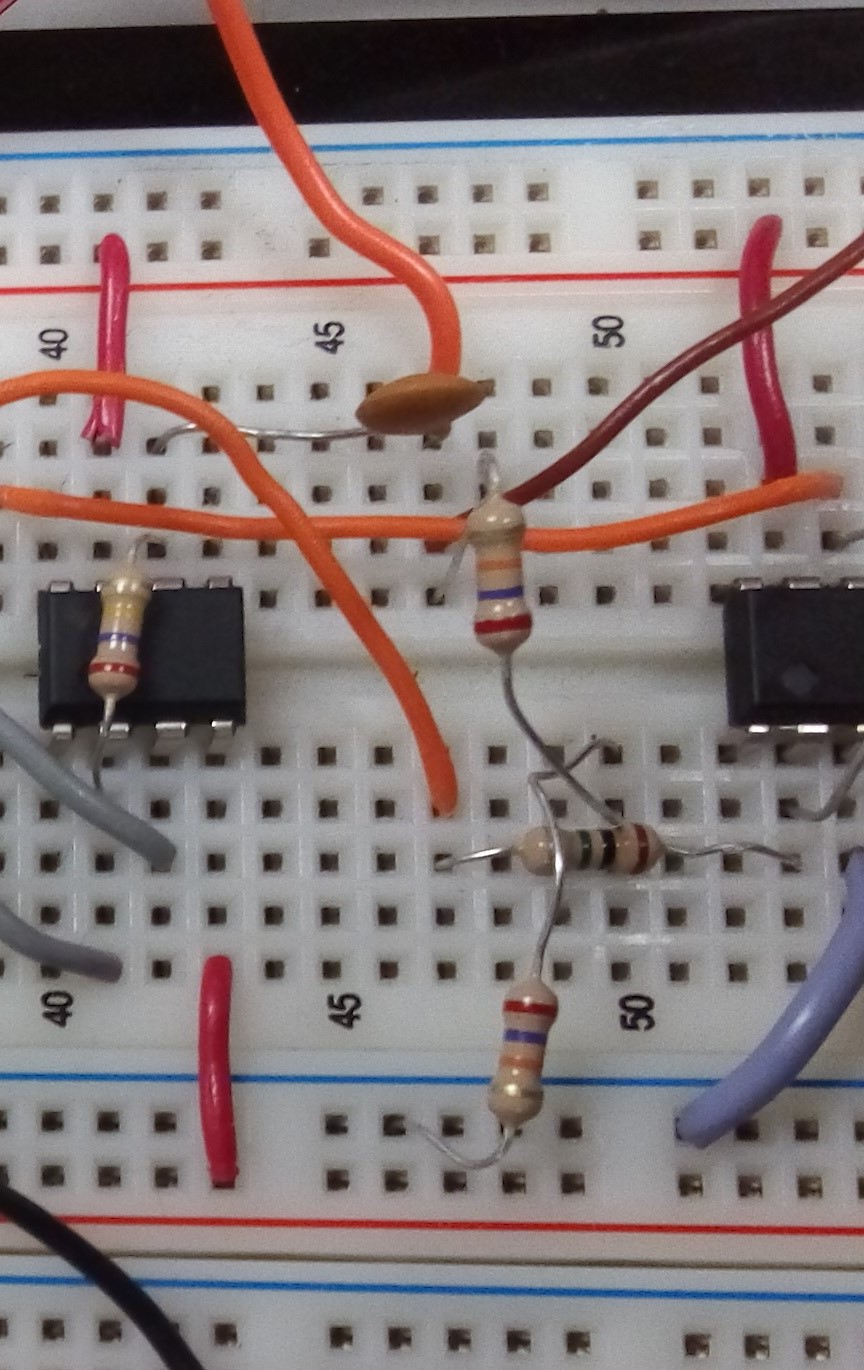
\includegraphics[scale=0.15]{Practica3/images/capacitor.jpg}
            \end{figure} 
            
            \item[\checkmark] En los 3 vídeos anexados a este reporte se puede visualizar a mayor detalle el \\ comportamiento y funcionamiento del circuito. Link: \url{https://drive.google.com/drive/folders/1Ip8R4pvErayRTnEQ73YYIijdkMI9oror?usp=sharing}
            \item[\checkmark] En cierto punto de la práctica, el electrodo a tierra se coloco en el tobillo del pie, en vez de la muñeca de la mano, y resulto en una mejor señal obtenida, más estable y con una respuesta al cambio de tensión muscular más rápida y adecuada. En el vídeo \textbf{VID\_03.3gp} se observa esta alteración en la medición.
    \end{itemize} 

	\newpage
	% /////////////////////////////////////////////////////////////////////
	%							CONCLUSIONES
	% ////////////////////////////////////////////////////////////////////
	\section{Conclusiones}
	    \subsection{Aguilar Herrera Arianna Itzamina}
	    En esta práctica se vuelve a utilizar el amplificador, el cuál ya sabemos como funciona, pues hemos estado trabajando con el en prácticas anteriores, pero, saliendo un poco de lo común vemos aplicaciones que puede tener un amplificador y la electrónica en sí. En esta ocasión se midió una variable de tipo fisiológica, mediante una señal mioeléctrica, es decir, una señal de contracción muscular.
	    
	    A pesar de que en la práctica podría decirse fue más para medir el esfuerzo que se realiza al hacer fuerza, puede dársele un mejor uso médico.
	    
	    Básicamente, a mayor escala, por supuesto, esto se aplica en la medicina, para medir la actividad eléctrica de los músculos, y si se continuara con el trabajo, lógicamente, se podría perfeccionar, y maximizar su uso. 
	    
	    \subsection{Nicolás Sayago Abigail}
	    En está práctica pudimos apreciar la forma en la que el amplificador de instrumentación ayuda en diferentes áreas, en esta práctica hablamos específicamente en la medicina.
	    
	    Al hacer la mediciones nuevamente notamos que existía un margen de error como en prácticas pasadas, también notamos como se comportan las señales que generan los músculos al ser procesadas por el amplificador de instrumentación, en ese proceso tuvimos algunos problemas como fue que en las primeras mediciones al meter la señal alterna el circuito estaba trabajando bien, pero al medir con un sujeto de prueba el circuito fallaba, finalmente notamos un falso en un electrodo y también se corrigió el filtro.
	    
	    En la parte del vúmetro también tuvimos problemas al pasar la señal, pero al final con ayuda del profesor logramos eliminar el ruido generado.
	    
	    Finalmente, logré observar nuevamente la utilidad de la instrumentación en las múltiples áreas.
	   
	    
	    \subsection{Ramos Diaz Enrique}
	    Un electromiograma es un una técnica muy importante en medicina, pues ayuda a detectar trastornos musculares y nerviosos entre los pacientes.
	    
	    En esta práctica, se utilizo el amplificador instrumentación para medir la señal mioeléctrica del brazo. Al contraer y relajar los músculos del cuerpo, se genera una ligera señal eléctrica; el gran problema aquí es que dicha señal esta llena de ruido.
	    
	    Para esto, el amplificador de instrumentación recibe dos entradas, una por cada electrodo colocado en la superficie del musculo de brazo. Posteriormente, aplica la diferencia entre ellas, eliminando el ruido.
	    
	    Al menos así es como teóricamente debería funcionar el circuito, pues con nosotros el ruido, a pesar de disminuir y atenuarse colocando el electrodo tierra en distintas posiciones del cuerpo (el tobillo del pie, por ejemplo) nunca se elimino por completo.
	    
	    Colocando el filtro y la adecuación extra a la señal de salida con el capacitor y las resistencias a tierra logramos estabilizar y atenuar la señal lo mejor posible. De este forma el osciloscopio desplegaba el cambio en la señal correctamente y los leds del vúmetro comenzaron a funcionar, pues antes de esto permanecían siempre encendidos.
	    
	    Por ultimo pero igual de importante, sufrimos algunos inconvenientes con los electrodos, ya que tenían falsos en el cable soldado a ellos, teniendo que mantenerlos colocados con el otro brazo para medir.
	    
	    

		\newpage
	%/////////////////////////////////////////////////////////////////
	%							ANEXOS
	%/////////////////////////////////////////////////////////////////
	
	\section{Anexos}
	    \subsection{Alimentación del circuito}
	        Todos los amplificadores operacionales LM741 de los circuitos deben estar alimentados por una fuente de +12 V y -12 V en serie. [Consultar hoja de especificaciones del LM741 para más información]. Deben ir dos capacitores de $10\mu F$, uno por cada entrada de voltaje.
	        
	        \begin{figure}[h!]
                \centering
                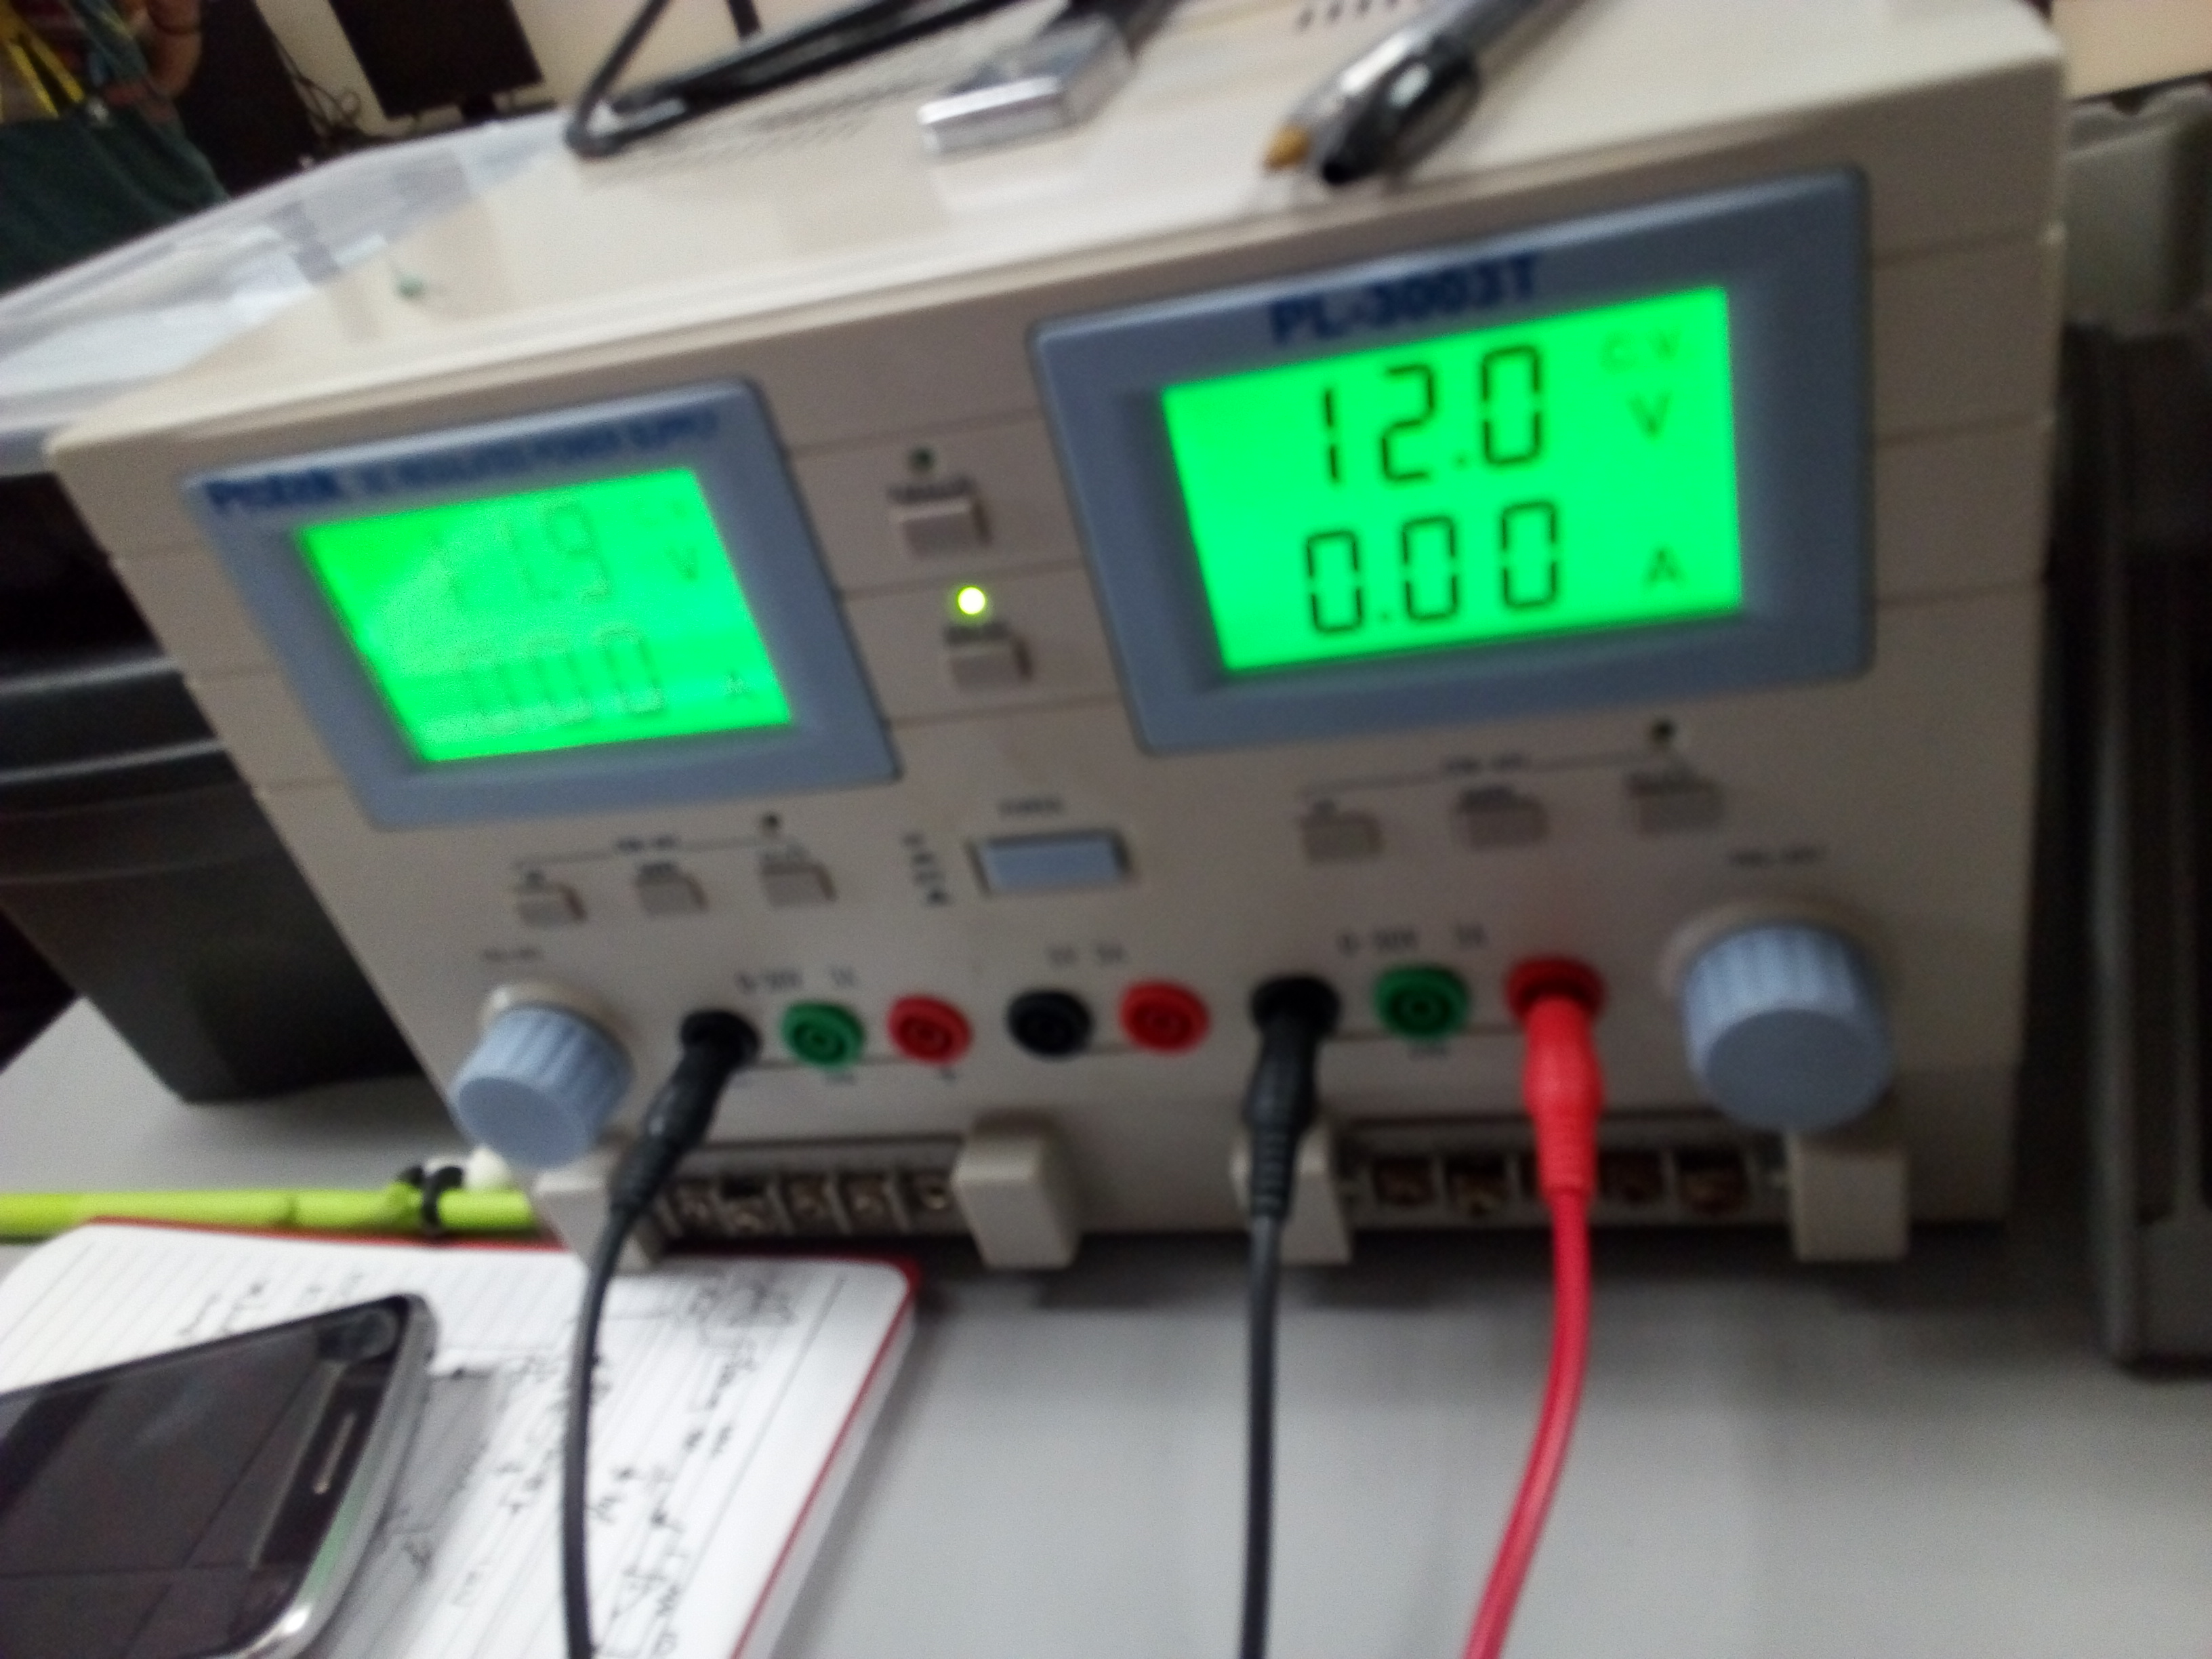
\includegraphics[width=0.7\textwidth]{Sismografo/Images/fuente.jpg}
            \end{figure} 
 
            \subsection{Electrodos}
            Se necesitan 3 electrodos, hechos a partir de una placa fenólica de cobre, para las mediciones del músculo del brazo en esta práctica. Deben poseer un cable soldado a la cara de cobre, barnizado y lijado para evitar corto circuitos o señales de entrada ajenas.
            
            La longitud de estos debe ser de 50 cm y dimensiones de entre 5x3 cm y 8x5 cm.
            \newpage
            \begin{figure}[h!]
                \centering
                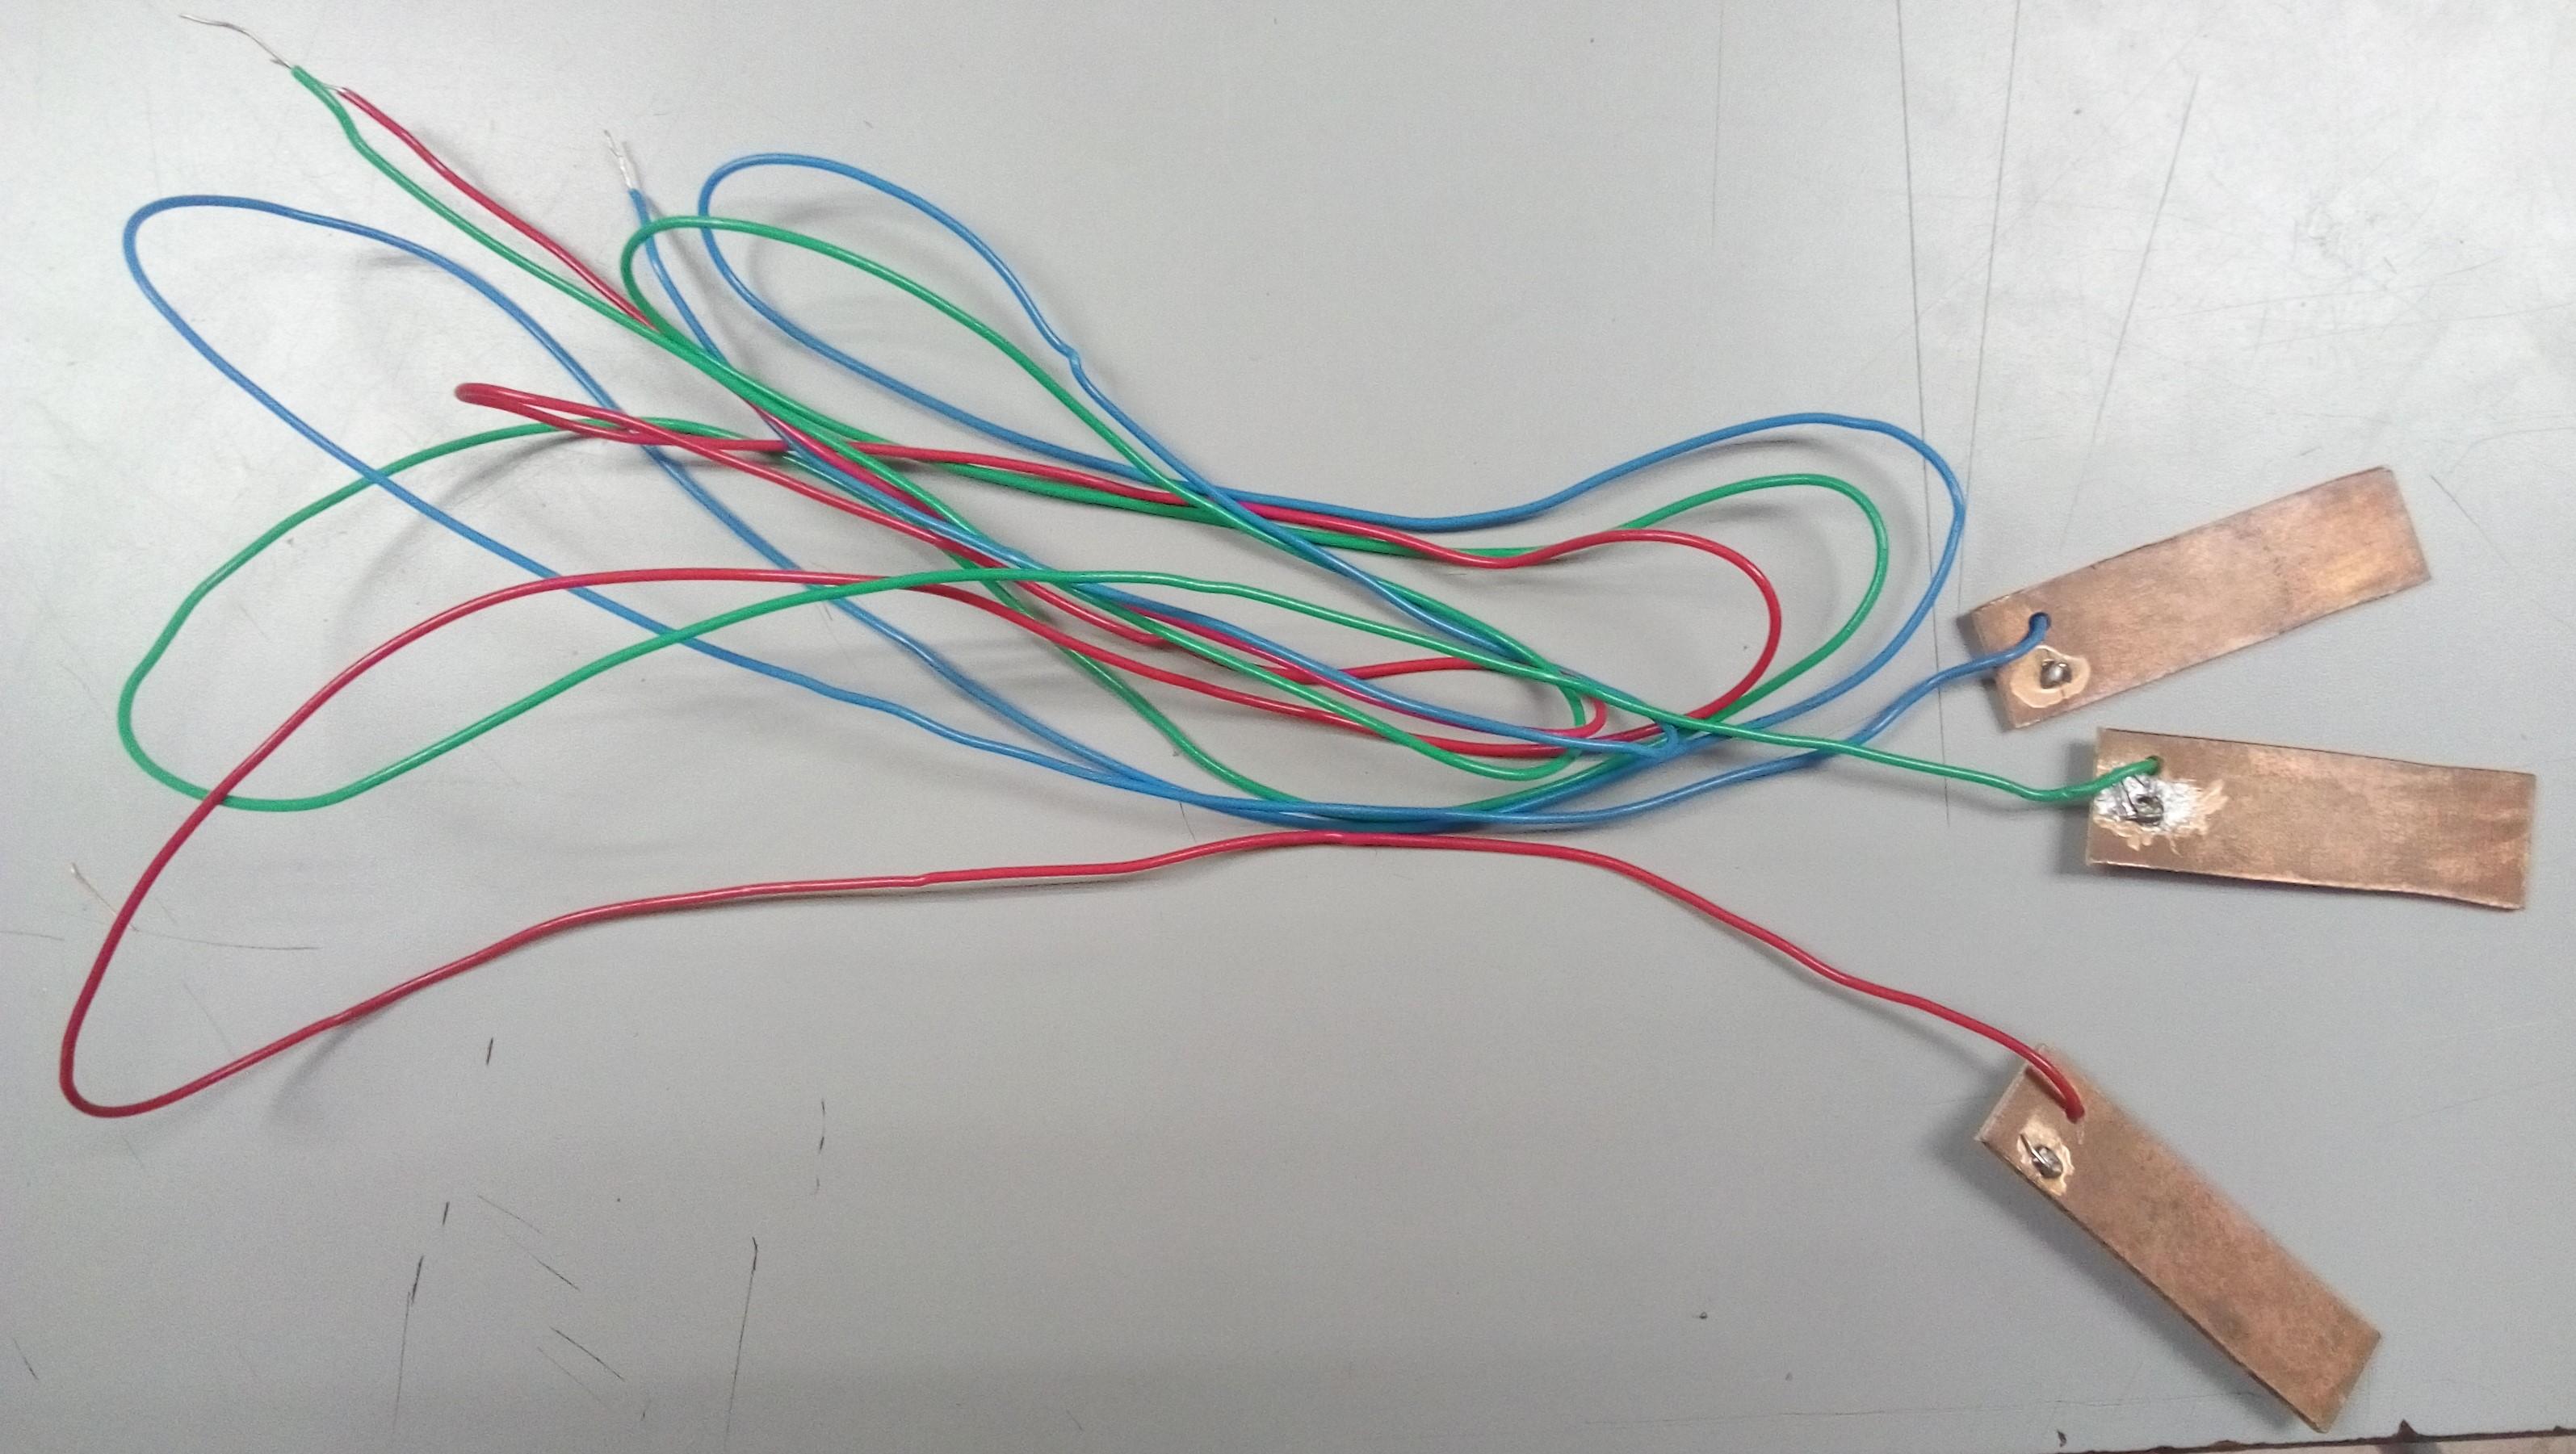
\includegraphics[width=0.75\textwidth]{Practica3/images/electrodos.jpg}
            \end{figure}
            
            %/////////////////////////////////////////////////////////////////
    	%          CALCULOS PROCEDIMIENTO EXPERIMENTAL 4
    	%/////////////////////////////////////////////////////////////////	    
		\subsection{PE- 3 Circuito 3: Vúmetro de led's}
		
		Para justificar nuestra repuesta en el procedimiento establecido, calculamos el rango con un divisor de Voltaje, como a continuación se muestra:
		
		\begin{enumerate}
		    \item Calculamos el voltaje de salida, y como las resistencias son iguales entonces aplicamos la siguiente ecuación:\\
		    Primero calculamos la Intensidad de corriente para:
		     $$
		        I = \frac{V}{R} = \frac{5V}{9(2.2k\Omega)} = \frac{5V}{19.8k\Omega} = 0.252 mA 
		     $$
		     Recordemos que el voltaje de la fuente de alimentación que va hacia las resistencias de las entradas inversoras de los amplificadores operacionales paso por un regulador de voltaje 7805 y ahora esta a 5V estables.
		     
		     Como es un circuito en serie, la corriente es la misma en todos por lo tanto al sacar el voltaje en cada uno de los operadores tenemos;
		   
		    \begin{equation*}
		        \begin{split}

		             V_{1} &= (R)I = RI = (2.2k\Omega)(0.252mA) = 0.55 V   \\
		            V_{2} &= (R+R)I = (2R)I = (4.4k\Omega)(0.252mA)) = 1.11 V     \\
		            V_{3} &= (R+R+R)I = (3R)I = (6.6k\Omega)(0.252mA) = 1.66 V     \\
		            V_{4} &= (R+R+R+R)I = (4R)I = (8.8k\Omega)(0.252mA) = 2.22 V     \\
		            V_{5} &= (R+R+R+R+R)I = (5R)I = (11k\Omega)(0.252mA) = 2.77 V     \\
		            V_{6} &= (R+R+R+R+R+R)I = (6R)I = (13.2k\Omega)(0.252mA) = 3.33 V     \\
		            V_{7} &= (7R)I = (15.4k\Omega)(0.252mA) = 3.88 V     \\
		            V_{8} &= (8R)I =  (17.6k\Omega)(0.252mA) = 4.44 V     \\

		        \end{split}
		    \end{equation*}
		    
		    Con estos cálculos, justificamos la respuesta de que el rango es de $0.55 V$ a $4.44 V$
		    
		\end{enumerate}

    %/////////////////////////////////////////////////////////////////
	%                           REFERENCIAS
	%/////////////////////////////////////////////////////////////////

	\nocite{ref1, ref2, ref3, ref4, ref5, ref6, ref7}
	\bibliography{refp3}
        

	\end{document}
